% !TEX program = xelatex
% Commands for running this example:
% 	 xelatex main
% 	 bibtex8 -W -c cp1256fa main
%      xindy -L persian -C utf8 -M texindy main
% 	 xelatex main
% 	 xelatex main
% End of Commands

%        نمونه پایان‌نامه آماده شده با استفاده از کلاس IUST-Thesis، نگارش 0.6
% 		محمود امین‌طوسی، دانشگاه تربیت معلم سبزوار، http://profsite.sttu.ac.ir/mamintoosi/
% 		گروه پارسی‌لاتک  http://www.parsilatex.com
%        این نسخه، بر اساس نسخه‌ 0.4 از کلاس Tabriz_Thesis آقای وحید دامن‌افشان آماده شده است. http://damanafshan.tk
%
%        تغییرات:
%        نسخه 0.6:
%        اصلاح مشکل بسته subfig
%----------------------------------------------------------------------------------------------
%        اگر قصد نوشتن پروژه کارشناسی را دارید، در خط زیر به جای msc، کلمه bsc و اگر قصد نوشتن پروژه دکترا
%        را دارید، کلمه phd را قرار دهید. کلیه تنظیمات لازم، به طور خودکار، اعمال می‌شود.

%        اگر مایلید پایان‌نامه شما دورو باشد به جای oneside  در خط زیر از twoside استفاده کنید
\documentclass[twoside,openright,msc]{ut_thesis}

% مشخصات پایان‌نامه را در فایلهای faTitle و enTitle وارد نمایید.

%       فایل commands.tex را مطالعه کنید؛ چون دستورات مربوط به فراخوانی بسته زی‌پرشین
%       و دیگر بسته‌ها و ... در این فایل قرار دارد و بهتر است که با نحوه استفاده از آنها آشنا شوید.
% در این فایل، دستورها و تنظیمات مورد نیاز، آورده شده است.
%-------------------------------------------------------------------------------------------------------------------
\usepackage{tabularx,ragged2e}
% در ورژن جدید زی‌پرشین برای تایپ متن‌های ریاضی، این سه بسته، حتماً باید فراخوانی شود
\usepackage{amsthm,amssymb,amsmath}
% بسته‌ای برای تنطیم حاشیه‌های بالا، پایین، چپ و راست صفحه
\usepackage[top=40mm, bottom=40mm, left=35mm, right=25mm]{geometry}
% بسته‌‌ای برای ظاهر شدن شکل‌ها و تصاویر متن
\usepackage{pdfpages}
\usepackage{graphicx}
% بسته‌ای برای رسم کادر
\usepackage{framed} 
% بسته‌‌ای برای چاپ شدن خودکار تعداد صفحات در صفحه «معرفی پایان‌نامه»
\usepackage{lastpage}
\usepackage{float}
% بسته‌ و دستوراتی برای ایجاد لینک‌های رنگی با امکان جهش
%\usepackage[pagebackref=false,colorlinks,linkcolor=blue,citecolor=blue]{hyperref}
% چنانچه قصد پرینت گرفتن نوشته خود را دارید، خط بالا را غیرفعال و  از دستور زیر استفاده کنید چون در صورت استفاده از دستور زیر‌‌، 
% لینک‌ها به رنگ سیاه ظاهر خواهند شد که برای پرینت گرفتن، مناسب‌تر است
\usepackage[pagebackref=false]{hyperref}
% بسته‌ لازم برای تنظیم سربرگ‌ها
\usepackage{fancyhdr}
%
\usepackage{setspace}
\usepackage{algpseudocode}
\usepackage{algorithm}
\usepackage{tikz}
%\usepackage{algorithmic}
%\usepackage[compatible]{algpseudocode}
\usepackage{subfigure}
\usepackage[subfigure]{tocloft}
\usepackage{afterpage}
% بسته‌ای برای ظاهر شدن «مراجع» و «نمایه» در فهرست مطالب
\usepackage[nottoc]{tocbibind}
% دستورات مربوط به ایجاد نمایه
\usepackage{makeidx}
\makeindex
%%%%%%%%%%%%%%%%%%%%%%%%%%
% فراخوانی بسته زی‌پرشین و تعریف قلم فارسی و انگلیسی
\usepackage{xepersian}
\settextfont[Path = fonts/, Scale=1]{XB Niloofar}
\setlatintextfont[Scale=0.9, Ligatures=TeX]{TeX Gyre Termes}%{Times New Roman}

%%%%%%%%%%%%%%%%%%%%%%%%%%
% چنانچه می‌خواهید اعداد در فرمول‌ها، انگلیسی باشد، خط زیر را غیرفعال کنید
%\setdigitfont[Scale=1]{XB Zar}%{Persian Modern}
%%%%%%%%%%%%%%%%%%%%%%%%%%
% تعریف قلم‌های فارسی و انگلیسی اضافی برای استفاده در بعضی از قسمت‌های متن
\defpersianfont\titlefont[Path = fonts/, Scale=1]{XB Titre}
% \defpersianfont\iranic[Scale=1.1]{XB Zar Oblique}%Italic}%
% \defpersianfont\nastaliq[Scale=1.2]{IranNastaliq}

%%%%%%%%%%%%%%%%%%%%%%%%%%
% دستوری برای حذف کلمه «چکیده»
\renewcommand{\abstractname}{}
% دستوری برای حذف کلمه «abstract»
%\renewcommand{\latinabstract}{}
% دستوری برای تغییر نام کلمه «اثبات» به «برهان»
%\renewcommand\proofname{\textbf{برهان}}
% دستوری برای تغییر نام کلمه «کتاب‌نامه» به «مراجع»
\renewcommand{\bibname}{مراجع}
% دستوری برای تعریف واژه‌نامه انگلیسی به فارسی
\newcommand\persiangloss[2]{#1\dotfill\lr{#2}\\}
% دستوری برای تعریف واژه‌نامه فارسی به انگلیسی 
\newcommand\englishgloss[2]{#2\dotfill\lr{#1}\\}
% تعریف دستور جدید «\پ» برای خلاصه‌نویسی جهت نوشتن عبارت «پروژه/پایان‌نامه/رساله»
\newcommand{\پ}{پروژه/پایان‌نامه/رساله }

%\newcommand\BackSlash{\char`\\}

%%%%%%%%%%%%%%%%%%%%%%%%%%
\SepMark{.}

% تعریف و نحوه ظاهر شدن عنوان قضیه‌ها، تعریف‌ها، مثال‌ها و ...
\theoremstyle{definition}
\newtheorem{definition}{تعریف}[section]
\theoremstyle{theorem}
\newtheorem{theorem}[definition]{قضیه}
\newtheorem{lemma}[definition]{لم}
\newtheorem{proposition}[definition]{گزاره}
\newtheorem{corollary}[definition]{نتیجه}
\newtheorem{remark}[definition]{ملاحظه}
\theoremstyle{definition}
\newtheorem{example}[definition]{مثال}

%\renewcommand{\theequation}{\thechapter-\arabic{equation}}
%\def\bibname{مراجع}
\numberwithin{algorithm}{chapter}
\def\listalgorithmname{فهرست الگوریتم‌ها}
\def\listfigurename{فهرست تصاویر}
\def\listtablename{فهرست جداول}

%%%%%%%%%%%%%%%%%%%%%%%%%%%%
% دستورهایی برای سفارشی کردن سربرگ صفحات
% \newcommand{\SetHeader}{
% \csname@twosidetrue\endcsname
% \pagestyle{fancy}
% \fancyhf{} 
% \fancyhead[OL,EL]{\thepage}
% \fancyhead[OR]{\small\rightmark}
% \fancyhead[ER]{\small\leftmark}
% \renewcommand{\chaptermark}[1]{%
% \markboth{\thechapter-\ #1}{}}
% }
%%%%%%%%%%%%5
%\def\MATtextbaseline{1.5}
%\renewcommand{\baselinestretch}{\MATtextbaseline}
\doublespacing
%%%%%%%%%%%%%%%%%%%%%%%%%%%%%
% دستوراتی برای اضافه کردن کلمه «فصل» در فهرست مطالب

\newlength\mylenprt
\newlength\mylenchp
\newlength\mylenapp

\renewcommand\cftpartpresnum{\partname~}
\renewcommand\cftchappresnum{\chaptername~}
\renewcommand\cftchapaftersnum{:}

\settowidth\mylenprt{\cftpartfont\cftpartpresnum\cftpartaftersnum}
\settowidth\mylenchp{\cftchapfont\cftchappresnum\cftchapaftersnum}
\settowidth\mylenapp{\cftchapfont\appendixname~\cftchapaftersnum}
\addtolength\mylenprt{\cftpartnumwidth}
\addtolength\mylenchp{\cftchapnumwidth}
\addtolength\mylenapp{\cftchapnumwidth}

\setlength\cftpartnumwidth{\mylenprt}
\setlength\cftchapnumwidth{\mylenchp}	

\makeatletter
{\def\thebibliography#1{\chapter*{\refname\@mkboth
   {\uppercase{\refname}}{\uppercase{\refname}}}\list
   {[\arabic{enumi}]}{\settowidth\labelwidth{[#1]}
   \rightmargin\labelwidth
   \advance\rightmargin\labelsep
   \advance\rightmargin\bibindent
   \itemindent -\bibindent
   \listparindent \itemindent
   \parsep \z@
   \usecounter{enumi}}
   \def\newblock{}
   \sloppy
   \sfcode`\.=1000\relax}}
\makeatother


\newcommand\blankpage{%
   \afterpage{
      \null
      \thispagestyle{empty}
      \newpage
   }
   \clearpage
}

\newcommand\cleartorightpage{
   \afterpage{
      \null
      \thispagestyle{empty}
      \ifodd\value{page}
         \clearpage \null
      \fi
      \newpage
   }
   \clearpage
}

\newcommand\cleartoleftpage{
   \afterpage{
      \null
      \thispagestyle{empty}
      \ifodd\value{page}
      \else
         \clearpage \null
      \fi
      \newpage
   }
   \clearpage
}

\usepackage{xecolor}
\usepackage{cleveref}
\crefformat{algorithm}{الگوریتم~(#2#1#3)}
\crefformat{figure}{شکل~(#2#1#3)}
\crefformat{table}{جدول~(#2#1#3)}
\crefformat{lemma}{لم~(#2#1#3)}
\crefformat{chapter}{فصل~(#2#1#3)}
\crefformat{equation}{رابطه~(#2#1#3)}
\crefformat{section}{بخش~(#2#1#3)}
\crefformat{line}{خط~#2#1#3}
\crefmultiformat{equation}{روابط~(#2#1#3)}{~و~(#2#1#3)}{،~(#2#1#3)}{~و~(#2#1#3)}
\crefrangeformat{equation}{روابط~(#3#1#4)~تا~(#5#2#6)}
\crefrangeformat{line}{خطوط~#3#1#4~تا~#5#2#6}

\newcommand{\argmax}[1]{\underset{#1}{\operatorname{arg}\,\operatorname{max}}\;}
\makeatletter
\newcommand{\algmargin}{\the\ALG@thistlm}
\makeatother
\algnewcommand{\parState}[1]{\State \parbox[t]{\dimexpr\linewidth-\algmargin}{\strut\hangindent=\algorithmicindent \hangafter=1 #1\strut}}
\setcounter{topnumber}{1}

\newcolumntype{C}{>{\Centering\arraybackslash}X} % centered "X" column

\fancyhead[RE,RO]{\leftmark}
\fancyhead[LO,LE]{\thesection}

\usepackage{zref-perpage}

\usepackage{remreset}
\makeatletter
\@removefromreset{footnote}{chapter}
\makeatother
\zmakeperpage{footnote}


\begin{document}

\pagenumbering{harfi}
% !TeX root=main.tex
\faculty{پردیس دانشکده‌های فنی}
\department{دانشکده مهندسی برق و کامپیوتر}
\subject{مهندسی برق}
\field{شبکه‌های مخابراتی}

\title{هوشمندی توزیع‌شده در شبکه‌های اینترنت اشیاء}
\firstsupervisor{دکتر وحید شاه‌منصوری}
%\secondsupervisor{استاد راهنمای دوم}
%\firstadvisor{استاد مشاور اول}
%\secondadvisor{استاد مشاور دوم}
\name{محمد}
\surname{محمودیان}
\studentID{810196391}
\thesisdate{شهریور 1399}
%\projectLabel{پایان‌نامه}
%\degree{}

\firstPage

\cleartorightpage
\besmPage

\cleartorightpage
\firstPage

\cleartorightpage
% \newpage

% \thispagestyle{empty}

%\includepdf{graphics/cert}
% \setcounter{page}{1}
% \vspace{-15cm}
% \begin{center}
%   \vspace{-5cm}
  
%   \makebox[\textwidth]{\vspace{-5cm}\includegraphics[width=\paperwidth]{graphics/cert}}
% \end{center}

 %\incgraph[width=\paperwidth]{graphics/cert}

 \davaranPage
\vspace{.5cm}
% در این قسمت اسامی اساتید راهنما، مشاور و داور باید به صورت دستی وارد شوند
\renewcommand{\arraystretch}{1.2}
 \begin{center}
   \begin{tabular}{|c|p{30mm}|c|c|p{25mm}|c|}
     \hline
     ردیف& سمت& نام و نام خانوادگی& مرتبه \newline دانشگاهی&دانشگاه یا مؤسسه& امضـــــــــــــا \\
     \hline
     ۱& استاد راهنما& دکتر وحید شاه‌منصوری& استاد‌یار& دانشگاه تهران                   &\\
     \hline
     ۲&‌استاد مدعو خارجی&دکتر&دانشیار& دانشگاه \newline صنعتی&                    \\
     \hline
     ۳& داور و نماینده \newline تحصیلات تکمیلی دانشکده & دکتر&استادیار                   & دانشگاه تهران& \\
     \hline
   \end{tabular}
 \end{center}

\cleartorightpage
\esalatPage

\cleartorightpage
\thispagestyle{empty}
{\Large تقدیم به:} \\
\begin{flushleft}
  {
    \huge
    پدر، مادر و خواهرم
  }
\end{flushleft}

\cleartorightpage
\begin{acknowledgementpage}
  سپاس خداوندگار حکیم را که با لطف بی‌کران خود، آدمی را زیور عقل آراست.

  در آغاز وظیفه‌ خود می‌دانم از زحمات بی‌دریغ استاد راهنمای خود، جناب آقای دکتر وحید شاه‌منصوری، صمیمانه تشکر و قدردانی کنم که قطعاً بدون راهنمایی‌های ارزنده‌ ایشان، این مجموعه به انجام نمی‌رسید.

  در پایان، بوسه می‌زنم بر دستان خداوندگاران مهر و مهربانی، پدر و مادر عزیزم و بعد از خدا، ستایش می‌کنم وجود مقدس‌شان را و تشکر می‌کنم از خانواده عزیزم به پاس عاطفه سرشار و گرمای امیدبخش وجودشان، که بهترین پشتیبان من بودند.
% با استفاده از دستور زیر، امضای شما، به طور خودکار، درج می‌شود.
\signature
\end{acknowledgementpage}

\keywords{اینترنت اشیاء، شهرهوشمند، پردازش لبه، تخصیص منابع، راه‌حل غیرمتمرکز، راه‌حل توزیع‌شده، قرارداد هوشمند}
\fa-abstract{
	شهرهوشمند یکی از کاربردهای مهم اینترنت اشیاءاست که اخیرا هم در عرصه تحقیقاتی و هم در عرصه صنعت مورد توجه خاص قرار گرفته‌است. در شهر هوشمند هدف این است که تمام دستگاه‌های موجود امکان اتصال به شبکه اینترنت را داشته باشند، تمام تبادل اطلاعات به صورت کاملا خودکار و در بستر این شبکه انجام شود. اطلاعات تولید شده توسط این دستگاه‌ها در قدم اول نیاز به پردازش و تحلیل دارد لذا لازم است این اطلاعات در بستر اینترنت به یک اپراتور ارسال شود و در ادامه اپراتور با تحلیل و پردازش داده های دریافتی تغییراتی را که باید در شبکه اعمال شوند به دستگاه های مرتبط ارسال کند.
	یکی از چالش های مهم در پیاده سازی الگوی شهر هوشمند، منابع و همچنین مکان مورد نیاز پردازش اطلاعات دریافتی است. از جمله ساده‌ترین راه‌حل‌های ارائه شده برای این چالش، پردازش کلیه‌ اطلاعات دریافتی در یک محل متمرکز به‌نام فضای ابری\LTRfootnote{Cloud} است. هرچند این روش متمرکز پردازش اطلاعات، با گسترش تعداد دستگاه‌ها و افزایش حجم اطلاعات، همچنین با به وجود آمدن سرویس‌های جدید که زمان پردازشی متفاوتی دارند، پاسخگوی نیاز اپراتورها نخواهد بود.
	به همین منظور پردازش لبه و پردازش مه به عنوان دو الگو پردازشی جدید مورد توجه محققان قرار گرفته اند. مهم ترین مزیت این دو الگوی پردازشی نسبت به پردازش ابری افزایش سرعت در پاسخ‌دهی به اطلاعات دریافتی است. اما با اضافه شدن این دو الگو پردازشی در کنار پردازش ابری مسئله تخصیص منابع برای پردازش اطلاعات به یکی از مهمترین چالش های اپراتور شبکه در استفاده از شهر هوشمند تبدیل شده است که مدلسازی و حل کردن آن نیازمند توان پردازشی زیادی‌است. پس از حل شدن این مسئله مشخص می‌شود که هر یک از گره‌های پردازشی موجود در شبکه، کدام بخش از اطلاعات موجود را پردازش کند. 
	در این پایان‌نامه مسئله تخصیص منابع مورد بررسی قرار می‌گیرد، مسئله اصلی درحالت کلی به صورت یک مسئله بهینه سازی غیرخطی ترکیب عددصحیح، که هدف آن کمینه کردن کل هزینه‌های شبکه است، مدل‌سازی می‌شود که این مسئله در دسته مسائل NP-hard قرار می‌گیرد. 
	مسئله خطی سازی می‌شود و به سه صورت متمرکز، غیرمتمرکز و توزیع‌شده حل می‌شود. راه‌حل‌های غیرمتمرکز و توزیع شده به صورتی هستند که از توان پردازشی گره‌های پردازشی استفاده می‌شود و نیازی نیست که یک واحد خارجی همه مسئولیت حل مسئله را برعهده بگیرد. این دو راه‌حل، همچنین این قابلیت را دارند که در شبکه زنجیره‌ بلوک، تحت عنوان قرارداد هوشمند پیاده‌سازی شوند.
	یک راه‌حل شبه‌بهینه نیز به صورت اکتشافی ارائه می‌شود که مسئله غیرخطی را مستقیما اما به‌صورت متمرکز حل می‌شود. 
}

\cleartorightpage
\abstractPage

\cleartorightpage

\setcounter{page}{1}
\tableofcontents
\newpage
\listoffigures \newpage
\listoftables  \newpage
%\input{others/acronyms}

\pagestyle{fancy}
% !TeX root=main.tex
% دستور زیر باید در اولین فصل شما باشد. آن را حذف نکنید!
\pagenumbering{arabic}

\chapter{مقدمه}
  \thispagestyle{empty}
	%todo    new subjects: all types of queuing systems and stability and queuing delay
	%todo sourced priorities
    اینترنت اشیاء(IoT\LTRfootnote{Internet of Things})امکان اتصال اشیاء هوشمند به یکدیگر را ممکن می‌سازد.
    اتصال این دستگاه‌های هوشمند به یکدیگر باعث می‌شود که این دستگاه‌ها بتوانند با یکدیگر و با اینترنت داده مبادله کنند.
    تبادل اطلاعات این امکان را ایجاد می‌کند که بتوانند خدمات متنوعی را برای کاربران فراهم کنند که قبلا امکان ارائه آن‌ها نبوده است.
    پیشرفت دستگاه‌های هوشمند و ظهور روش‌های جدید پردازش داده، اینترنت اشیاء را به عنوان گزینه‌ای مناسب برای استفاده در شهر هوشمند\LTRfootnote{Smart city} ، شبکه هوشمند انرژی\LTRfootnote{Smart grid}، خانه هوشمند\LTRfootnote{Smart home} و سلامتی هوشمند\LTRfootnote{Smart health} قرار داده است.
    امروزه یکی از مسائل پرطرفدار در اینترنت اشیاء، شهر هوشمند است که در آن هدف این است که کلیه وسائل موجود به نحوی هوشمند شده و ارتباطات بین آن‌ها به دور از نقش انسان و به صورت کاملا مکانیزه انجام شود.
    به دلیل علاقه دولت‌‌ها برای استفاده از اینترنت اشیاء در بهبود مدیریت امور عمومی، شهر هوشمند به عنوان بهترین راهکار تحقق وسیع اینترنت اشیاء در نظر گرفته می‌شود.

    یکی از مهم‌ترین بخش‌های اینترنت اشیاء، پردازش داده‌هایی است که توسط حسگر‌های مختلف جمع‌آوری شده‌ اند.
    به طور سنتی پردازش ابری\LTRfootnote{Cloud Computing} روشی کارا برای پردازش داده بوده است چرا که ظرفیت پردازشی ابر بسیار بیشتر از دیگر روش‌های پردازشی است.
    با این حال، افزایش چشمگیر در تعداد دستگاه‌های هوشمند و افزایش وسیع در میزان حجم اطلاعات موجود جهت پردازش و همچنین کافی نبودن پهنای باند شبکه‌ها برای انتقال حجم انبوه داده‌های تولید شده در اینترنت اشیاء باعث می‌شود که انتقال داده‌ها و پردازش همه‌ی آن‌ها در فضای ابری به عنوان گلوگاه پردازش ابری باشد.
    به همین دلیل، ارسال همه‌ی داده‌ها برای پردازش به فضای ابری، می‌تواند باعث زمان پاسخ طولانی سرویس‌ها شود که برای بسیاری از سرویس‌ها قابل قبول نیست.
    از پردازش لبه\LTRfootnote{Edge Computing} و پردازش مه\LTRfootnote{Fog Computing} به عنوان راه‌حل‌هایی برای این مشکل یاد می‌شود.
    در پردازش لبه هدف این است که پردازش داده‌ها تا حد ممکن در جایی که داده‌ها تولید می‌شوند انجام شود.
    پردازش مه نیز مشابهت زیادی به پردازش لبه دارد با این تفاوت که فاصله گره‌های پردازشی تا حسگرها نسبت به پردازش لبه بیشتر است. 

    در یک شبکه اینترنت اشیاء تعداد بسیار زیادی حسگر\LTRfootnote{Sensor}‌ و فعال‌کننده\LTRfootnote{Actuator}‌ مانند حسگر‌های دود\LTRfootnote{Smoke sensors}، حسگر‌های دما\LTRfootnote{Temperature sensors}، حسگر‌های حرکت\LTRfootnote{Motion sensors}، دوربین‌های نظارتی و هشدار‌های خطر آتش وجود دارند.
    همچنین سرویس‌های\LTRfootnote{Services} زیادی هم وجود دارند که از داده‌های این حسگر‌ها استفاده و با پردازش این داده‌ها، نتیجه‌هایی را تولید می‌کنند.
    برای هر سرویس، داده‌های حسگر‌ها باید به یک منبع پردازشی ارسال شوند و بعد از پردازش نتیجه به مقصد‌های مورد نظر فرستاده شوند.
    این مقصد‌ها می‌توانند فعال‌کننده‌ها یا ذخیره‌سازهای ابری و غیره باشند.
    به عنوان نمونه می‌توان سرویس تشخیص آتش سوزی را نام برد.
    در این سرویس، ورودی‌ها می‌توانند حسگر‌های دود،حسگرهای دما و دوربین‌های ویدیویی باشند و هشداردهنده‌‌های آتش، خروجی باشند.
    قسمت پردازش، ورودی حسگر‌ها و دوربین‌ها را مورد بررسی قرار می‌دهد و هشدار دهنده‌ها را فعال می‌کند یا می‌تواند به ایستگاه‌‌های آتشنشانی اطلاع دهد.  
    به عنوان نمونه‌ی دیگر، سرویس‌های امنیت ساختمان‌ها را در نظر بگیرید.
    در این سرویس‌ها، داده‌های حسگر‌های حرکتی و دوربین‌های نظارتی پردازش می‌شوند و در صورت تشخیص نفوذ غیر مجاز هشدار دهنده‌ها فعال می‌شوند و به پلیس اطلاع داده می‌شود.
    اطلاعات ورودی هر سرویس را می‌توان در قالب مجموعه‌ای از بسته‌ها و تحت عنوان وظیفه\LTRfootnote{Task} درنظر گرفت که هر وظیفه ویژگی‌ها و قیدهای مشخص و مخصوص به خود را دارد.
    
    هرچقدر تعداد اطلاعات ارسالی مربوط به یک محیط بیشتر باشد می‌توان گفت که احتمال بروز خطا در محاسبات کمتر می‌شود زیرا تصمیم‌گیری صرفا براساس اطلاعات مربوط یه یک حسگر انجام نمی‌شود.
    
    سرویس‌ها برای پردازش داده‌های خود باید در منابع پردازشی مناسب پردازش شوند به‌طوری‌که تمام قیدهای مربوط به آن‌ها به بهترین وجه ممکن برآورده شود. 
    تعداد بسیار زیاد سرویس‌ها و منابع پردازشی در شبکه اینترنت اشیاء باعث می‌شود که مسئله پیدا کردن منبع پردازشی بهینه برای سرویس‌ها، یک مسئله پیچیده باشد.
    به همین دلیل در این پایان نامه به بررسی و ارائه راه حل برای حل مسئله اختصاص منابع پردازشی در اینترنت اشیاء می‌پردازیم.

    \section{اینترنت اشیاء و شهر هوشمند}
    واژه‌ی اینترنت اشیاء برای اولین بار توسط کوین اشتون\LTRfootnote{Kevin Ashton} در یک ارائه برای استفاده از بازشناسی با امواج رادیویی\LTRfootnote{RFID} در مدیریت زنجیر تأمین\LTRfootnote{Supply Chain} استفاده شد\cite{shton2009that}.
    اینترنت اشیاء امکان اتصال هر کسی در هر مکان و زمانی به هر چیزی در هر مکانی و هر زمانی را فراهم می‌کند.
    با پیشرفت تکنولوژی به سمت جامعه‌ای پیش می‌رویم که همه افراد و همه‌ی اشیاء متصل خواهند بود\cite{zheng2011internet}.
    ایده‌ی اصلی اینترنت اشیاء این است که امکان اتصال خودکار و امن و انتقال داده‌ بین دستگاه‌های فیزیکی و برنامه‌های کاربردی را فراهم می‌کند.
    در واقع اینترنت اشیاء این امکان را ایجاد می‌کند که اشیاء فیزیکی بتوانند ببینند، بشنوند، و با صحبت کردن با یکدیگر بتوانند تصمیم‌گیری کنند و کار‌هایی را انجام دهند\cite{al2015internet}.
    در طول زمان انتظار می‌رود اینترنت اشیاء کاربرد‌های خانگی و تجاری فراوانی داشته باشد، کیفیت زندگی افراد را بهبود ببخشد و باعث رشد اقتصاد جهانی بشود.

    هدف اینترنت اشیاء این است که اینترنت را فراگیرتر و همه جانبه‌تر کند.
    علاوه بر این، به وسیله‌ی دسترسی آسان و تعامل با طیف گسترده‌ای از دستگاه‌هایی مانند لوازم خانگی، دوربین‌های نظارتی، حسگر‌ها، فعال‌کننده‌ها، نمایشگر‌ها، خودرو‌ها و غیره، اینترنت اشیاء به توسعه‌ی کاربرد داده‌های تولید شده توسط این دستگاه‌ها برای فراهم کردن خدمات به شهروندان، شرکت‌ها و اداره‌ی امور عمومی کمک می‌کند.
    این الگو، کاربرد‌هایی در حوزه‌های مختلف مانند اتوماسیون خانگی، اتوماسیون صنعتی، کمک‌های پزشکی، سلامت همراه، نگهداری از افراد سالمند، مدیریت هوشمند انرژی و شبکه هوشمند، وسایل نقلیه، مدیریت ترافیک و موارد دیگر دارد \cite{bellavista2013convergence}.
    
    در چنین عرصه‌ی ناهمگونی از کاربرد‌ها،پیداکردن یک راه‌حل که بتواند به همه‌ی نیاز‌های کاربرد‌های مختلف پاسخ بدهد، چالش برانگیز خواهد بود.
    دشواری پیدا کردن این راه‌حل باعث ایجاد راه‌حل‌های متفاوت و بعضاً ناسازگار برای تحقق سامانه‌های اینترنت اشیاء شده است \cite{zanella2014internet}.
    بنابر این از دید سیستمی، به دلیل نوآوری‌ها و پیچیدگی‌های اینترنت اشیاء، نیاز به تحقق یک شبکه‌ی اینترنت اشیاء، به همراه شبکه سرویس‌ها و شبکه دستگاه‌ها وجود دارد.
    علاوه بر مشکلات فنی، عدم وجود یک مدل تجاری مورد قبول که بتواند سرمایه‌گذاران را برای ترویج استقرار این تکنولوژی‌ها جذب کند مانع توسعه سریع استفاده از اینترنت اشیاء شده است\cite{laya2013investing}.

    در این سناریوی پیچیده، کاربرد اینترنت اشیاء در محیط‌های شهری، از محبوبیت بالایی برخوردار است چرا که به تقاضای بسیاری از دولت‌ها برای استفاده از فناوری‌ اطلاعات و ارتباطات در مدیریت امور عمومی پاسخ می‌دهد و باعث می‌شود مفهومی که از آن با عنوان شهر هوشمند یاد می‌شود، تحقق یابد \cite{schaffers2011smart}.
    در حالی که هنوز تعریفی که موردقبول همگان برای شهر هوشمند باشد وجود ندارد، هدف نهایی استفاده‌ی بهتر از منابع عمومی، افزایش کیفیت خدمات ارائه شده به شهروندان و کاهش هزینه‌های عملیاتی مدیریت امور عمومی است. 
    این اهداف به کمک اینترنت اشیاء شهری قابل دستیابی خواهند بود.
    منظور از اینترنت اشیاء شهری، زیرساخت ارتباطی است که دسترسی یکپارچه، ساده و اقتصادی را به مجموعه‌ای از خدمات عمومی فراهم می‌کند.
    اینترنت اشیاء شهری می‌تواند مزایایی در مدیریت و بهینه‌سازی خدمات عمومی مرسوم مانند حمل و نقل و پارک خودرو‌ها، روشنایی، نظارت و نگهداری اماکن عمومی، حفظ آثار باستانی، جمع آوری پسماند، بیمارستان‌ها و مدارس داشته‌باشد.
    علاوه براین، وجود انواع مختلف داده‌های جمع‌آوری شده توسط یک اینترنت اشیاء شهری فراگیر، می‌تواند برای افزایش شفافیت استفاده شود، اقدامات تصمیم‌گیران محلی را ترویج دهد، آگاهی شهروندان راجع به وضعیت شهرشان را بیشتر کند، شهروندان را به مشارکت فعال در مدیریت عمومی تشویق کند و باعث خلق سرویس‌های جدیدی علاوه بر سرویس‌های فراهم شده توسط اینترنت اشیاء بشود \cite{cuff2008urban}.
    بنابراین استفاده از اینترنت اشیاء به صورت خاص برای تصمیم‌گیران محلی و منطقه‌ای جذاب است و باعث می‌شود که آن‌ها اولین استفاده کننده‌های این تکنولوژی‌ها باشند و به عنوان کاتالیزور برای انطباق الگوی اینترنت اشیاء در مقیاس‌های بزرگ‌تر عمل کنند.

  \section{خدمات شهر هوشمند}
    در ادامه برخی از خدماتی که امکان ارائه‌ی آن‌ها توسط اینترنت اشیاء شهری فراهم می‌شود را مرور می‌کنیم.
    \subsection{نظارت بر سلامت ساختار ساختمان‌ها}
      نگهداری مناسب ساختمان‌های تاریخی شهر‌ها نیاز به نظارت مداوم وضعیت واقعی ساختمان‌ها و پیدا‌کردن‌ مکان‌هایی که بیشترین تاثیر را از عوامل خارجی دریافت می‌کنند دارد.
      اینترنت اشیاء شهری می‌تواند یک پایگاه داده‌ی توزیع شده از اندازه‌گیری‌های یکپارچگی ساختاری ساختمان‌ها فراهم ‌کند که به وسیله‌ی حسگر‌های مناسبی که در نقاط مختلف ساختمان نصب شده‌اند، اندازه‌گیری شده‌اند.
      این حسگر‌ها می‌توانند، لرزش و تغییر شکل، رطوبت و دما را اندازه‌گیری کنند و شرایط محیطی را به طور کامل مشخص کنند\cite{lynch2006summary}.
      این پایگاه داده باید بتواند هزینه بالای لازم برای آزمایش دوره‌ای مقاومت ساختمان‌ها توسط عوامل انسانی را کاهش دهد و امکان نظارت فعال بر وضعیت ساختمان‌ها را فراهم کند.
      همچنین امکان ترکیب کردن اطلاعات لرزش ساختمان‌ها و اطلاعات مربوط به زمین لرزه‌های کوچک برای بررسی و فهم تاثیر آن‌ها بر ساختمان‌ها فراهم می‌شود.
      با این وجود تحقق عملی این خدمت، نیاز به نصب حسگر‌هایی در ساختمان‌ها و محیط‌های اطراف و ارتباطشان با یک مرکز کنترل دارد که ممکن است نیاز به یک سرمایه‌گذاری اولیه برای ایجاد این زیرساخت‌ها داشته باشد.

    \subsection{مدیریت پسماند}
      هزینه‌ی بالای خدمات مدیریت پسماند و مشکلات نگهداری پسماند در محل‌های دفن زباله باعث می‌شود که مدیریت پسماند یکی از مهم‌ترین مشکلات در بیشتر شهر‌های بزرگ می‌باشد.
      نفوذ بیشتر راه‌حل‌های مبتنی بر فناوری‌های ارتباطات و اطلاعات در این حوزه می‌تواند به طور چشمگیری باعث کاهش هزینه‌ها بشود و بهبود‌هایی در زمینه‌های اقتصادی و زیست محیط داشته باشد.
      برای مثال استفاده از سطل‌های زباله هوشمند که امکان اندازه‌گیری وزن محتویات درون سطل را دارند و امکان بهینه‌سازی فرآیند جمع‌آوری پسماند را فراهم میکنند، می‌توانند هزینه‌ی جمع‌آوری پسماند را کاهش دهند و کیفیت بازیافت پسماند را بیشتر کنند \cite{nuortio2006improved}.
      برای رسیدن به یک سرویس جمع‌آوری پسماند هوشمند، اینترنت اشیاء باید بتواند سطل‌های زباله هوشمند را به یک مرکز کنترل وصل کند.
      در این مرکز کنترل یک نرم‌افزار بهینه‌سازی اجرا می‌شود تا مدیریت بهینه کامیون‌های جمع‌آوری پسماند را مشخص کند.

    \subsection{نظارت بر کیفیت هوا}
      اتحادیه اروپا به صورت رسمی اهدافی را برای کاهش تغییرات اقلیمی در دهه آینده تعیین کرده است.
      از آن‌ها می‌توان به کاهش ۲۰ درصدی در تولید گاز‌های گلخانه‌ای در سال ۲۰۲۰ میلادی نسبت به سال ۱۹۹۰، کاهش ۲۰ درصدی مصرف انرژی با بهبود بهره‌وری انرژی و افزایش ۲۰ درصدی استفاده از انرژی‌های تجدید‌پذیر را نام برد.
      در زمینه کیفیت هوا، اینترنت اشیاء می‌تواند روش‌هایی برای پایش کیفیت هوای مناطق پر ازدحام و پارک‌ها ارائه دهد \cite{al2010mobile}.
      علاوه بر این‌ها امکانات ارتباطی می‌توانند برای برنامه‌های روی دستگاه‌های هوشمند دوندگان امکان ارتباط با زیرساخت‌های لازم را فراهم کنند.
      به کمک این زیرساخت‌ها، افراد می‌توانند سالم‌ترین مسیر برای فعالیت‌های خارج از منزل را پیدا کنند.
      تحقق خدماتی از این قبیل نیازمند نصب حسگر‌های آلودگی و کیفیت هوا در نقاط مختلف شهر و قرارگیری داده‌های این حسگر‌ها به صورت عمومی در اختیار شهروندان است.

    \subsection{نظارت بر آلودگی صوتی}
      مسئولین شهری معمولا قوانینی برای کاهش آلودگی صوتی در مراکز شهر برای برخی ساعات تصویب می‌کنند.
      اینترنت اشیاء شهری می‌تواند یک سرویس نظارت بر آلودگی صوتی ارائه دهد که وظیفه‌ی آن اندازه‌گیری سطح آلودگی صوتی در ساعتی مشخص در مناطقی که این سرویس در آن‌ها برقرار است، باشد \cite{maisonneuve2009citizen}.
      همچنین این سرویس با استفاده از الگوریتم‌های تشخیص صدا می‌تواند شکستن شیشه‌ها و یا صدای نزاع خیابانی را تشخیص دهد و با این کار باعث افزایش امنیت بشود.
      با این حال نصب حسگر‌های صوتی به دلیل مسائل مربوط به حریم شخصی می‌تواند حساسیت بر انگیز باشد.

    \subsection{مدیریت ترافیک}
      از دیگر خدمات شهر هوشمند که به وسیله‌ی اینترنت اشیاء شهری قابل دستیابی است، به نظارت بر ترافیک شهر می‌توان اشاره کرد.
      با این که نظارت ویدیویی ترافیک در حال حاظر در بیشتر شهر‌ها استفاده می‌شود، استفاده از شبکه‌های گسترده کم توان می‌تواند منبع انبوهی از اطلاعات را در اختیار قرار دهد.
      نظارت بر ترافیک می‌تواند با نصب سامانه‌های موقعیت یاب بر روی خودرو‌های جدید تحقق یابد \cite{li2008performance} و با خدمات نظارت بر کیفیت هوا و نظارت بر آلودگی صوتی ترکیب شود.
      این اطلاعات، اهمیت زیادی برای مسئولین و شهروندان خواهد داشت چرا که باعث افزایش نظم و برنامه ریزی بهتر می‌شود.

    \subsection{نظارت بر مصرف انرژی در شهر}
      در کنار نظارت بر کیفیت هوا، اینترنت اشیاء شهری می‌تواند خدماتی برای نظارت بر مصرف انرژی تمام شهر ارائه کند.
      با این کار شهروندان و مسئولین می‌توانند یک گزارش دقیق از میزان انرژی مورد نیاز برای سرویس‌های مختلف (روشنایی عمومی، حمل و نقل، چراغ‌های راهنمایی و رانندگی، دوربین‌های نظارتی، گرمایش و سرمایش ساختمان‌های عمومی و غیره) داشته باشند.
      این کار می‌تواند امکان شناسایی منابع اصلی مصرف انرژی را فراهم سازد تا بتوان برای بهینه‌سازی رفتار آن‌ها چاره‌ای پیدا کرد.
      برای ممکن ساختن این خدمات، دستگاه‌های نظارت بر میزان مصرف انرژی باید با شبکه‌های قدرت یکپارچه بشوند.
      هم چنین امکان کنترل فعال منابع تولید انرژی مانند صفحات خورشیدی می‌تواند باعث بهبود این خدمات بشود.

    \subsection{پارک هوشمند}
      خدمات پارک هوشمند، مبتنی بر حسگر‌های خیابان‌ها و نمایشگر‌های هوشمند است که رانندگان خودرو‌ها را به بهترین جای پارک در شهر هدایت می‌کند \cite{lee2008intelligent}.
      از مزایای این خدمت می‌توان کاهش زمان لازم برای برای پیدا کردن جای پارک و در نتیجه کاهش انتشار گاز CO از ماشین‌ها، کاهش ترافیک و افزایش رضایت شهروندان اشاره کرد.
      این خدمات می‌توانند به صورت مستقیم در زیرساخت اینترنت اشیاء شهری ادغام شوند چرا که تولید کنندگان، دستگاه‌های لازم برای آن را آماده کرده‌اند.
      این خدمات امکان شناسایی افراد معلول و ارائه‌ی خدمت ویژه به آن‌ها را فراهم می‌کند.
      مثلا اجازه استفاده از پارکینگ‌های خاص و یا ارائه‌ی ابزار‌هایی برای مشخص کردن سریع استفاده غیر مجاز از پارکینگ‌ها.

    \subsection{روشنایی هوشمند}
      برای کاهش انرژی مصرفی شهر، استفاده بهینه از روشنایی بسیار مهم است.
      به طور خاص این خدمت می‌تواند شدت روشنایی خیابان‌ها را مطابق ساعت روز، وضعیت هوا و حضور افراد تنظیم کند.
      این خدمت برای این که به درستی کار کند نیاز به این دارد که اطلاعات روشنایی شهر را در زیرساخت شهر هوشمند ترکیب کند.
      از دیگر مزایای آن این است که امکان شناسایی ساده خطا در سامانه روشنایی شهر در این روش وجود خواهد داشت.

    \subsection{اتوماسیون ساختمان‌های عمومی}
      یکی از کاربرد‌های تکنولوژی‌های اینترنت اشیاء نظارت بر مصرف انرژی ساختمان‌های عمومی (مدارس، دفاتر مدیریت عمومی و موزه‌ها) و بهبود شرایط محیطی برای فعالیت افراد است.
      برای این منظور از انواع متفاوتی از حسگر‌ها و فعال‌کننده‌هایی که نور، دما و رطوبت را کنترل می‌کنند استفاده می‌شود.
      با کنترل این پارامتر‌ها، علاوه بر کاهش هزینه‌ی گرمایش و سرمایش، سطح آسایش افرادی که در این محیط‌ها کار می‌کنند افزایش پیدا می‌کند که خود می‌تواند باعث افزایش بهره‌وری افراد شود \cite{lee2008intelligent}.

  \section{سرویس‌ها و وظیفه‌ها}
    سرویس‌های موجود در شهر هوشمند را می‌توان از چند نظر تقسیم بندی کرد. یکی از انواع این تقسیم‌بندی ها تقسیم‌بندی برمبنای کیفیت مورد انتظار(QoS\LTRfootnote{Quality of Service}) است. به این صورت که یک سری معیار به عنوان معیارهای کمی مشخص می‌شود که لازم است این سرویس‌ها به گونه‌ای باشند که این معیارها را تا حد خوبی برآورده سازند. از جمله‌ی این معیارهای کمی می‌توان به تاخیر مربوط به انجام سرویس اشاره کرد. 
    تاخیر هر سرویس خود چند بخش مختلف دارد. در مورد سرویس اطفا حریق می‌توان گفت که ابتدا لازم است که حسگرها اطلاعات پیرامون خود را جمع‌آوری کنند سپس این اطلاعات جمع‌آوری شده به مرکز پردازشی ارسال شود و در آنجا این اطلاعات پردازش شود و نتیجه‌ی اطلاعات به فعال‌کننده ارسال شود و درنهایت آن‌ها شروع به اقدام کنند در تمام این مراحل تاخیرهای مختلف وجود دارد.
    با توجه به رشد خیلی خوب این روزها در ساختار دستگاهِ‌های الکترونیکی می‌توان گفت که دستگاه‌های خیلی دقیق و سریعی در بازار موجود است که با کمترین خطا درحال دریافت اطلاعات و همچنین انجام کارهای مربوطه هستند و بحث مربوط به افزایش بازدهی در این دستگاه‌ها در گرایش‌های مربوط به رشته‌ی الکترونیک می‌تواند بحث جذابی باشد، لذا در این پایان نامه از تاخیرهای مربوط به عملکرد حسگرها و فعال‌کننده‌ها صرف‌‌نظر شده است و فرض براین است که این دستگاه‌ها به محض دریافت اطلاعات بلافاصله کار خود را انجام می‌دهند. اما در مورد انواع دیگر تاخیر لازم است که دقت لازم انجام گیرد که در ادامه به تفصیل بیشتر دراین مورد صحبت خواهد شد.
    
    \subsection{انواع تاخیر در شبکه‌های سوئیچ بسته}
    در این بخش قرار است که انواع مختلف تاخیر در شبکه‌های سوئیچ بسته بررسی شود . 
    در این شبکه‌ها یک بسته ارسالی، سفر خود را از یک میزبان (مبدأ) شروع می‌کند، از تعدادی سوییچ و مسیریاب می‌گذرد و در پایان سفر خود، به میزبان دیگر (مقصد) می‌رسد. با حرکت بسته از یک گره\LTRfootnote{Node} (میزبان یا مسیریاب) به گره دیگر در طول مسیر، در هر گره انواع مختلفی از تاخیر می‌تواند برای بسته در حال ارسال اتفاق بیفتد.
    این تاخیر ها عبارتند از
    \begin{enumerate}
    	\item \textbf{تاخیر پردازش:}
    مدت زمانی است که طول می‌کشد یک گره، بسته دریافتی را تحلیل کند و بفهمد که آیا لازم است آن را به سمت یک گره دیگر هدایت کند و یا اینکه خودش آن را پردازش کند. همچنین اگر زمانی صرف بررسی سالم بودن بیت‌های موجود در بسته شود این زمان جزء این دسته از تاخیر قرار می‌گیرد.
    \item \textbf{تاخیر صف:}
    تاخیری است که بسته‌ها درصف ورودی منتظر می‌شوند تا نوبت پردازش آن‌ها برسد که میزان این تاخیر با توجه به فرمول‌های مربوط به تئوری صف و نوع صف و همچنین مدل پردازشی گره محاسبه می‌شود. همچنین درصورتی که گره موجود، یک گره مسیریاب باشد یعنی عملکرد آن به صورتی باشد که بسته‌های دریافتی را به سایر گره‌ها هدایت می‌کند ممکن است در خروجی این گره نیز یک صف تشکیل شود و بسته در آن صف خروجی هم مقداری منتظر بماند.
    \item \textbf{تاخیر انتقال:} 
    این تاخیر برابر است با مدت زمان لازم برای انتقال کلیه‌ی بیت‌های موجود در بسته بر روی لینک‌های موجود که همانطور که می‌دانیم در حالت ساده شده با فرض اینکه بسته ارسالی شامل $L$ بیت باشد و همچنین آهنگ انتقال لینک به اندازه $R$ بیت بر ثانیه باشد آن‌گاه تاخیر انتقال این بیت به اندازه‌ی$\frac{L}{R}$ ثانیه خواهد بود. 
    \item \textbf{تاخیر انتشار:} 
    به محض آن‌که مسیریاب A یک بیت را روی لینک خروجی فرستاد، این بیت باید تا مسیریاب B منتشر شود. زمان لازم برای منتشر شدن این بیت از ابتدای لینک تا مسیریاب B را تاخیر انتشار می‌گویند.
    سرعت حرکت بیت‌ها روی یک لینک در واقع همان سرعت انتشار امواج الکترومغناطیسی در لینک است، که به نوع رسانه فیزیک مورد استفاده در لینک (فیبر نوری، زوج به هم تابیده، بی سیم و …) بستگی دارد.
    تاخیر انتشار در یک لینک ارتباطی برابر است با فاصله بین دو مسیریاب (طول لینک که با $d$ نشان می‌دهند) تقسیم بر سرعت انتشار $s$ یعنی $\frac{d}{s}$.
    \end{enumerate}
    تاخیر انتقال زمان لازم برای بیرون دادن تمامی بیت های یک بسته توسط مسیریاب است و به صورت تابعی از طول بسته و آهنگ انتقال به لینک خروجی در مسیریاب تعریف می‌شود؛ در نتیجه هیچ ارتباطی با فاصله بین دو مسیریاب (یا همان طول لینک) ندارد.
    از طرفی، تاخیر انتشار زمانی است که طول می‌کشد تا یک بیت از یک مسیریاب به مسیریاب بعدی برسد، این تاخیر تابعی از فاصله بین دو مسیریاب و سرعت انتشار امواج الکترومغناطیسی در رسانه فیزیکی لینک می باشد و هیچ ارتباطی با طول بسته یا آهنگ انتقال لینک ندارد.
    معمولا در مقالات مربوط به شبکه‌های بی‌سیم از تاخیر انتشار در مقابل تاخیر انتقال صرف نظر می‌شود و یا این دو تاخیر را به عنوان یک تاخیر در نظر می‌گیرند. در این پایان‌نامه نیز این دو تاخیر به صورت جدا درنظر گرفته نشده‌اند و عملا از تاخیر انتشار صرف‌نظر شده است. 
    
  \section{پردازش لبه}
    گسترش اینترنت اشیاء و موفقیت سرویس‌های ابری باعث ایجاد الگو‌ی جدیدی در پردازش داده‌ها به نام پردازش لبه \LTRfootnote{Edge Computing} شده است.
    در این الگوی پردازشی سعی بر این است که پردازش داده‌ها در لبه شبکه انجام شود.
    طبق براورد‌های انجام شده در \cite{2018cisco} تعداد دستگاه‌های متصل شده به شبکه ۵۰ میلیارد عدد خواهد بود.
    بعضی از کاربردهای اینترنت اشیاء نیاز به زمان پاسخ کوتاه دارند، بعضی ممکن است دارای داده‌های محرمانه وشخصی باشند و بعضی از این کاربرد‌ها می‌توانند بار سنگینی برای شبکه داشته باشند و پردازش ابری ممکن است روش مناسبی برای این کاربرد‌ها نباشد.

    \subsection{چرا به پردازش لبه نیاز داریم؟}
      در حال حاظر نرخ تولید داده در لبه شبکه در حال افزایش می‌باشد.
      بنابراین پردازش این داده‌ها در لبه شبکه روش کارامدتری خواهد بود.
      در ادامه دلایلی برای لزوم استفاده از پردازش لبه را بر می‌شماریم \cite{shi2016edge}:
      \begin{description}
        \item [فشار از سمت پردازش ابری:]
          قرار دادن همه وظایف پردازش در ابر به عنوان یک روش کارآمد برای پردازش داده‌ها شناخته شده است چرا که قدرت پردازشی ابر قابل مقایسه با قدرت پردازشی اشیاء در لبه شبکه نیست.
          با این حال، در مقایسه با پیشرفت سریع سرعت پردازش داده‌ها، پهنای‌باند شبکه‌ها تقریبا ثابت مانده‌اند.
          افزایش تولید داده در لبه شبکه باعث شده است که انتقال این داده‌ها به گلوگاه پردازش ابری تبدیل شود.
          به عنوان مثال یک اتومبیل خودران را در نظر بگیرید.
          در هر ثانیه ۱ گیگابایت داده توسط آن تولید می‌شود و پردازش بلادرنگ\LTRfootnote{Real-Time} این داده‌ها برای تصمیم‌گیری درست لازم است.
          اگر قرار باشد که همه این داده‌ها برای پردازش به ابر فرستاده شوند، زمان پاسخ بسیار طولانی خواهد بود.
          علاوه بر این، پهنای باند و قابلیت اطمینان شبکه‌های فعلی برای پردازش داده‌‌های تعداد زیادی خودرو در یک منطقه کافی نخواهد بود.
          در این موارد داده‌ها باید در لبه شبکه پردازش شوند.
          این کار زمان پاسخ کوتاه‌تر، پردازش کارآمد‌تر و فشار کم‌تر بر شبکه را به ارمغان می‌آورد.

        \item [کشش از سمت اینترنت اشیاء:]
          انتظار می‌رود که تعداد اشیاء لبه شبکه به میلیارد‌ها دستگاه برسد.
          در نتیجه داده‌های خام تولید شده توسط آن‌ها حجم بسیار بزرگی خواهند داشت و این حجم بزرگ باعث می‌شود که روش‌های مرسوم پردازش ابری مناسب برای پردازش این حجم از داده‌ها نباشند.
          در نتیجه می‌توان درنظر گرفت که بیشتر این داده‌های تولید شده در اینترنت اشیاء هیچ وقت برای پردازش به ابر ارسال نمی‌شوند و در لبه شبکه پردازش می‌شوند.

          \cref{fig:chapter_2:cloud_paradigm} ساختار مرسوم در پردازش ابری را نشان می‌دهد.
          تولید کننده‌های داده، داده‌های خام را به ابر انتقال می‌دهند.
          مصرف کننده‌ها هم با ارسال درخواست نتیجه را از ابر به‌دست می‌آورند.
          با این حال این ساختار برای استفاده در اینترنت اشیاء مناسب نیست.
          اولا حجم داده‌ی تولید شده در لبه شبکه بسیار زیاد است که پهنای باند شبکه و منابع پردازشی زیادی را طلب می‌کند.
          ثانیا حفظ حریم شخصی به عنوان یک مانع برای پردازش ابری ایجاد می‌کند.
          در انتها، بسیاری از گره‌های انتهایی در اینترنت اشیاء دارای انرژی محدودی هستند و ماژول‌های مخابرات بی‌سیم معمولا مصرف انرژی بالایی نیاز دارند.
          در نتیجه انجام وظایف پردازشی در لبه شبکه می‌تواند از لحاظ مصرف انرژی بهینه‌ باشد.

          \begin{figure}[h]
            \centerline{\includegraphics[width=10cm]{graphics/chapter_2/cloud_paradigm}}
            \caption{الگوی پردازش ابری \cite{shi2016edge}}
            \label{fig:chapter_2:cloud_paradigm}
          \end{figure}

        \item [تغییر از مصرف کننده داده به تولید کننده داده:]
          در الگوی پردازش ابری، دستگاه‌های انتهایی در لبه شبکه معمولا نقش مصرف کننده داده را دارند.
          به عنوان نمونه می‌توان تماشای یک ویدیو را مثال زد.
          با این حال امروزه مردم در حال تولید داده توسط دستگاه‌هایشان هستند.
          برای مثال امروزه بسیار عادی است که افراد عکس‌ها و ویدیو‌هایی که توسط خودشان ضبط شده است را در سرویس‌های اینترنتی مختلف به اشتراک بگذارند.
          در \cite{2019domo} اشاره شده است که در هر دقیقه در \lr{twitter} ۵۱۱۲۰۰ توییت جدید ارسال می‌شود و در \lr{instagram} ۵۵۱۴۰ عکس جدید بارگذاری می‌شود.
          باید توجه داشت که این تصاویر و ویدیوها می‌توانند حجم زیادی داشته باشند و پهنای باند زیادی را برای بارگذاری استفاده کنند.
          در این موارد ویدیو‌ها باید ابتدا حجمشان در لبه شبکه کاهش پیدا کند تا به وضوح تصویر\LTRfootnote{Resolution} مناسب برای بارگذاری در شبکه برسند.
          به عنوان نمونه‌ی دیگر می‌توان دستگاه‌های مربوط به سلامت را مثال زد.
          داده‌های جمع‌آوری شده توسط این دستگاه‌ها معمولا خصوصی است و پردازش این داده‌ها در لبه شبکه به جای ارسال داده‌ها برای پردازش به ابر به حفظ حریم خصوصی افراد کمک می‌کند.

      \end{description}
    
    \subsection{پردازش لبه چیست؟}
      پردازش لبه به همه تکنولوژی‌هایی اطلاق می‌شود که امکان انجام پردازش‌ داده‌ها در لبه شبکه را فراهم می‌کنند.
      در اینجا منظور از لبه، همه منابع پردازشی و شبکه ای است که بین منبع داده‌ها (جایی که داده‌ها در آن جا تولید می‌شوند) و مراکز داده‌ی ابری قرار دارند.
      برای مثال یک دروازه‌ی شبکه در یک خانه هوشمند، می‌تواند یک منبع پردازشی لبه بین اشیاء و مرکز داده‌ی ابری باشد یا یک مرکز داده‌ی کوچک، می‌تواند یک منبع پردازشی لبه بین دستگاه‌های سیار و ابر در نظر گرفته شود.
      منطق در پردازش لبه این است که پردازش داده‌ها باید در همسایگی منبع داده‌ها انجام شود.
      با این منطق پردازش لبه و پردازش مه دو مفهوم یکسان را خواهند داشت با این تفاوت که پردازش لبه تمرکزش سمت اشیاء است ولی پردازش مه تمرکزش سمت زیرساخت است.

      \begin{figure}[h]
        \centerline{\includegraphics[width=10cm]{graphics/chapter_2/edge_paradigm}}
        \caption{الگوی پردازش لبه \cite{shi2016edge}}
        \label{fig:chapter_2:edge_paradigm}
      \end{figure}
      
      \cref{fig:chapter_2:edge_paradigm} جریان پردازش دو طرفه را در پردازش مه نشان می‌دهد.
      در الگو پردازش لبه، اشیاء نه تنها مصرف کننده داده بلکه تولید کننده‌ داده نیز هستند.
      در واقع در لبه، اشیاء نه تنها می‌توانند سرویس و محتوا از ابر درخواست نمایند بلکه می‌توانند وظایف پردازشی را هم انجام دهند.

    \subsection{مزایای پردازش لبه}
      هدف از پردازش لبه قراردادن پردازش در مجاورت منبع تولید داده‌ها است.
      این کار مزایایی نسبت به روش‌های مبتنی بر پردازش ابری مرسوم دارد.
      در \cite{yi2015fog} برنامه‌ای برای تشخیص چهره ساخته شده است که با انتقال پردازش از ابر به لبه شبکه، زمان پاسخ برنامه از ۹۰۰ به ۱۶۰ میلی ثانیه کاهش پیدا کرده است.
      در \cite{ha2014towards} نویسندگان از واحدهای پردازشی ابری کوچک\LTRfootnote{Cloudlet} برای پردازش وظایف دستیار شناختی پوشیدنی\LTRfootnote{Wearable Cognetive Assitance} استفاده کرده اند و نتایج نشان می‌دهد که زمان پاسخ بین ۸۰ تا ۲۰۰ میلی ثانیه کاهش پیدا کرده است.
      روش ارائه شده در \cite{chun2011clonecloud} برای اجرای برنامه‌های تلفن همراه به کمک استفاده همزمان از پردازش ابری و پردازش لبه توانسته زمان اجرا و انرژی مصرفی را تا ۲۰ برابر کاهش دهد.

    \subsection{کاربرد پردازش لبه در شهر هوشمند}
      ویژگی‌های زیر باعث می‌شوند که پردازش لبه برای استفاده در شهر هوشمند مناسب باشد.
      \begin{enumerate}
        \item \textbf{حجم زیاد داده:}
          تخمین زده می‌شود که در سال ۲۰۱۹ میلادی یک شهر با جمعیت ۱ میلیون نفر، ۱۸۰ پتابایت داده در هر روز تولید می‌کند\cite{index2015forecast}.
          این داده‌ها توسط امنیت عمومی، سلامت، تجهیزات شهری و حمل و نقل تولید می‌شوند.
          ساختن مراکز داده‌ی متمرکز برای رسیدگی به همه‌ی این داده‌ها یک راهکار غیر واقعی است چرا که از این حجم از داده نیاز به قدرت پردازشی بسیار زیادی دارد.
          در این مورد پردازش لبه می‌تواند یک راه حل بهینه برای پردازش این حجم عظیم از داده‌ها باشد.

        \item \textbf{تاخیر کم:}
          برای کاربرد‌هایی که نیاز به تاخیر قابل پیشبینی و کم دارند مانند اورژانس سلامتی و امنیت عمومی، پردازش لبه یک الگوی مناسب است چرا که زمان انتقال داده‌ها را کاهش می‌دهد و ساختار شبکه را ساده‌تر می‌کند
        \item \textbf{آگاهی از مکان:}
          برای کاربرد‌های مبتنی بر موقعیت جغرافیایی مانند حمل و نقل و مدیریت تجهیزات شهری پردازش لبه به دلیل آگاهی از مکان، بهتر از پردازش ابری عمل می‌کند.
      \end{enumerate}
  
  \section{پردازش مه}
  شرکت Cisco برای اولین بار، پردازش مه را در ماه ژانویه سال 2014 معرفی کرد. ایده‌ی پشت پردازش مه نسبت به پردازش ابری، افزایش سرعت پردازش اطلاعات بود. ریشه پردازش مه، همان پردازش ابری است، با این تفاوت که به دلیل سرعت بالاتر انتقال اطلاعات، در فناوری‌هایی مثل اینترنت اشیا مورد استفاده قرار می‌گیرد.
  
  هم‌زمان با رشد و نفوذ دستگاه‌های اینترنت اشیا در حوزه‌های مختلف، استفاده از خدمات پردازش مه نیز در این حوزه اهمیت بیشتری یافت. پیش‌بینی می‌شود فناوری پردازش مه که محاسبات مه هم گفته می‌شود، در آینده رشد قابل توجهی داشته باشد. گزارشی از 451 تحقیق انجام شده در این زمینه نشان داد که بازار پردازش مه تا سال 2022 به ارزشی برابر 4/6 میلیارد دلار خواهد رسید.
  
  \subsection{عملکرد پردازش مه چگونه است؟}
  دستگاه‌هایی که در مه وجود دارند تحت عنوان گره شناخته می‌شوند. هر دستگاه با ارتباط شبکه‌ای، محاسباتی و ذخیره‌سازی می‌تواند یک گره باشد که در هر جایی با یک ارتباط شبکه‌ای می‌توانند قرار گیرند. دستگاه‌های مختلف از کنترل‌کننده‌ها تا مسیریاب‌ها و دوربین‌های فیلمبرداری، می‌توانند به عنوان یک گره مه عمل کنند. این گره‌ها می‌توانند در مناطق هدف مانند دفتر کار یا در یک وسیله نقلیه به‌کار گرفته شوند. وقتی یک دستگاه اینترنت اشیا داده‌هایی تولید می‌کند، این داده‌ها می‌توانند از طریق یکی از این گره‌ها دریافت شوند و در شبکه، پردازش سپس به مراکز داده ابری منتقل ‌شوند.
  
  تفاوت اصلی میان پردازش ابری و پردازش مه این است که محاسبات مه نزدیکی جغرافیایی بیشتری به کاربر نهایی دارد و توزیع جغرافیایی وسیع‌تری ایجاد می‌کند.
  
  \subsection{مزایای پردازش مه}
  دلایل مختلفی برای به‌کارگیری پردازش مه وجود دارد. این دلایل در نهایت باعث افزایش بهره‌وری سازمانی می‌شوند. در ادامه به برخی از مهم‌ترین مزایای بکارگیری پردازش مه می‌پردازیم.
  \begin{itemize}
  \item \textbf{کاهش زمان تاخیر:}
  یکی از بزرگ‌ترین مزایای پردازش مه، کاهش زمان تاخیر است. دیگر لازم نیست داده‌ها برای پردازش به مراکز داده ابری فرستاده شوند و از بین رفتن این مشکل باعث می‌شود که تحلیل و پردازش داده‌ها بسیار بهتر و موثرتر انجام شود.
  
  \item \textbf{کاهش ملزومات عملکردی:}
  عدم ارسال داده‌ها به مراکز داده پردازش ابری علاوه بر صرفه‌جویی در زمان، می‌تواند میزان پهنای باند لازم برای این کار را هم کاهش دهد و در مقابل، این میزان پهنای باند برای ارتباط با حسگرها و مراکز داده ابری بکار برده شود. این روش در نهایت باعث کاهش ملزومات عملکرد می‌شود.
  
  \item \textbf{توزیع جغرافیایی گسترده:}
  استفاده از پردازش مه با تمرکززدایی از شبکه، امکان توزیع جغرافیایی گسترده‌تری را نسبت به شبکه‌سازی سنتی یا پردازش ابری فراهم می‌آورد. این کار به ارایه سرویس با کیفیت‌تر برای کاربر نهایی منجر می‌شود.
  
  \item \textbf{تحلیل در لحظه:}
  در بسیاری از محیط‌ها، توانایی تحلیل فوری داده‌ها، اهمیت بسیار زیادی دارد. حذف عوامل ناکارآمدی و تاخیر که در سرویس‌های خدمات ابری وجود دارند، به معنای آن است که کاربر می‌تواند تحلیل معتبر و لحظه‌ای داده‌ها را در اختیار داشته باشد.
    \end{itemize}
  
  \section{انواع لایه در شبکه}
  با توجه به مطالب گفته شده می‌توان گفت که لایه‌های شبکه را می‌توان به دو دسته تقسیم کرد. دسته‌ی اول لایه‌های مربوط به تولید و جمع‌آوری اطلاعات و دسته‌ی دوم لایه‌های مربوط به پردازش اطلاعات.
  در این پایان‌نامه لایه‌های مربوط به دسته‌ی اول را یک لایه در نظر می‌گیریم که شامل کلیه‌ی حسگرها و فعال‌کننده‌هاست. در مورد دسته دوم سه لایه‌ی لبه، مه و ابری را در نظر می‌گیریم. که به ترتیب فاصله از لایه‌ی حسگر قرار گرفته‌اند.   
 
  در مورد تفاوت بین لایه‌ لبه و لایه مه علاوه بر بحث تفاوت در فاصله و میزان تاخیر می‌توان گفت که ظرفیت پردازشی در لایه‌ی مه از لایه‌ی لبه بیشتر است. همچنین در این پایان‌نامه یک هزینه پردازشی برای گره‌های محاسباتی در نظر گرفته شده‌است به این صورت که به صورت میانگین هزینه‌ی پردازشی در گره‌های لبه از دولایه دیگر بیشتر است و گره‌های موجود در لایه‌ی ابری ارزان‌ترین هزینه پردازشی را دارند. 
  
  دربعضی از تعاریف لایه‌ی لبه را یک لایه مجازی بر روی لایه‌ی حسگر در نظر می‌گیرند به این صورت که اطلاعات حسگرها فراتر از لایه‌ی آن‌ها نمی‌رود و درهمان لایه پردازش می‌شود مزیتی که این فرض دارد جنبه‌ی امنیت و محافظت از اطلاعات است. اما در این پایان‌نامه لایه‌ی لبه را جدا از لایه‌ی جسگر درنظر گرفته‌ایم. 
   
  حال صورت مسئله‌ای که ایجاد می‌شود این است که با توجه به حق انتخاب‌های موجود و با توجه به اطلاعات حسگرها که لازم است پردازش شوند مناسب ترین مکان برای پردازش این اطلاعات کجاست.
 
  انتخاب مکان مناسب برای پردازش بستگی به تعریف دقیق صورت مسئله و همچنین تعریف دقیق از کیفیت سرویس‌ها دارد. به عنوان مثال می‌توان هدف را این‌گونه در نظر گرفت که شبکه به صورتی کار کند که اطلاعات حسگرها در کمترین زمان ممکن پردازش شود که در این صورت احتمالا قیدی بر روی هزینه‌ی لازم برای پردازش اطلاعات لازم است که درنظر گرفته شود که در نتیجه‌ی آن، نمی‌توان گفت که شبکه در ارزان‌ترین حالت خود به سر می‌برد.
  در یک حالت دیگر می‌توان صورت مسئله را به‌گونه‌ای طراحی کرد که هزینه‌های کلی شبکه در بهینه‌ترین حالت ممکن باشد. در این صورت لازم است که شرایط مربوط به تاخیر به عنوان قید به صورت مسئله اضافه شوند. در هر دوحالت مدلسازی قبل این بحث به وجود می‌آید که آیا شبکه توان پردازش کلیه‌ی اطلاعات حاصل از لایه‌ی حسگرها را دارد یا نه، که لازم است این قسمت نیز به عنوان قید به مسئله اصلی اضافه شود.  در حالتی دیگر می‌توان صورت مسئله را به این صورت تعریف کرد که تعداد پردازش‌ها بیشترین مقدار ممکن باشد. 

  \section{نو‌آوری‌های پایان نامه}
    دستاورد‌های این پایان‌نامه را می‌توان به صورت زیر خلاصه کرد:
    در بخش اول، صورت مسئله‌ی یافتن مکان مناسب برای پردازش اطلاعات با هدف بهینه کردن هزینه‌های کل شبکه مدل‌سازی شده است و مسئله به صورت یک مسئله بهینه‌سازی غیرخطی ترکیبی عددصحیح نوشته شده‌است. ابتدا مسئله خطی‌سازی شده و به‌صورت مرکزی حل‌شده است. سپس یک راه‌حل غیرمتمرکز ارائه شده‌است. 

    در بخش دوم، ابتدا یک راه‌حل اکتشافی برای صورت مسئله غیرخطی نوشته شده‌است. در ادامه صورت مسئله‌ خطی شده به‌صورت توزیع‌شده حل‌ می‌شود.  


  \section{ساختار پایان‌نامه}
    ساختار پایان‌نامه به شرح زیر است.

    \cref{chap:literature_review} به مروری بر مطالعات انجام شده در زمینه تخصیص منابع اینترنت اشیاء می‌پردازد.
    
    \cref{chap:system_model_centralized_decentralized} به بررسی مسئله اختصاص منابع پردازشی باتوجه به مدل ارائه شده می‌پردازد.
    در این فصل مسئله بهینه‌سازی همراه با تمام قیدهای موجود نوشته می‌شود، درنهایت مسئله خطی‌سازی می‌شود، به صورتی‌که که حل کردن آن راحت‌تر باشد. 
    درادامه مسئله به صورت غیرمتمرکز بازنویسی می‌شود و یک الگوریتم غیرمتمرکز ارائه می‌شود. 

    در \cref{chap:heuristic_distributed} مسئله تخصیص منابع پردازشی به دو صورت دیگر مورد بررسی قرار گرفته است.
    ابتدا یک الگوریتم اکتشافی مبتنی بر روش viterbi ارائه می‌شود، مزیت این روش این است که نیازی نیست خطی سازی انجام شود و از اولین فرم مسئله که غیرخطی است، می‌توان استفاده کرد. 
    در ادامه یک الگوریتم توزیع‌شده ارائه می‌شود و مجددا مسئله توسط آن الگوریتم حل و بررسی می‌شود. 

    در انتها در \cref{chap:conclusion} به بیان نتیجه‌گیری و کار‌های آینده می‌پردازیم.
\chapter{مروری بر مطالعات انجام شده}\label{chap:literature_review}
  \thispagestyle{empty}
  در این فصل ابتدا مدل سیستم این پایان نامه را معرفی می‌کنیم و سپس مقالاتی را که به تخصیص منابع در شبکه اینترنت اشیاء پرداخته‌اند بررسی می‌کنیم.

  در این پایان نامه فرض می‌کنیم که تعدادی وظیفه وجود دارند.
  هر وظیفه، مشخصات معین مربوط به خود را دارد و لازم است اطلاعات مربوط به این وظیفه پردازش شود. 
  برای پردازش داده‌های وظیفه‌ها باید منابع پردازشی به آن‌ها اختصاص پیدا کنند.
  مسئله تخصیص منابع در این پایان نامه به صورت یک مسئله بهینه سازی فرمول بندی شده است که تابع هدف آن کمینه کردن مجموع هزینه منابع پردازشی می‌باشد. 
  در این تابع هدف، هزینه هر گره، با توجه به نوع و تعداد وظیفه‌هایی که پردازش می‌کند و باتوجه به نوع گره مدل‌سازی می‌شود. 

  \section{تخصیص منابع پردازشی در شبکه اینترنت اشیاء}
    مقاله \cite{sarkar2016theoretical}، یک فرمول بندی ریاضی برای پردازش مه ارائه می‌دهد.
    برای این کار اجزاء مختلف را تعریف می‌کند و به مطالعه‌ی تفاوت‌های پردازش مه با پردازش ابری مرسوم می‌پردازد.
    مدل سیستم این مقاله در \cref{fig:chapter_2:system_model_sarkar2016theoretical} رسم شده است.
    همانطور که از این شکل مشخص است، در این مقاله سیستم از سه لایه تشکیل شده است.
    در لایه اول دستگاه‌های اینترنت اشیاء قرار دارند که وظیفه جمع‌آوری داده‌های حسگر‌ها و وقایع و ارسال داده‌های خام به گره بعدی را دارند.
    لایه دوم که به عنوان لایه مه معرفی شده است از دستگاه‌هایی مانند مسیریاب‌ها و نقاط دسترسی\LTRfootnote{Access Point} تشکیل شده است که می‌توانند داده‌ها را پردازش و به صورت موقت ذخیره کنند.
    این دستگاه‌ها به چهارچوب‌های ابری متصل هستند و مسئول ارسال اطلاعات به صورت متناوب به ابر می‌باشند.
    در لایه سوم پردازش ابری قرار دارد که بالاترین لایه می‌باشد و شامل تعدادی منبع پردازشی با ظرفیت بالا می‌باشد که می‌توانند حجم زیادی از داده‌‌ها را پردازش و ذخیره سازی کنند.
    با بررسی انجام شده، پردازش مه به کمک پردازش ابری می‌تواند پاسخ گوی نیاز نسل بعدی کاربرد‌های اینترنت اشیاء باشد.
    نتایج مورد مطالعه نشان می دهند که زمانی که ۲۵٪ کاربرد‌های اینترنت اشیاء نیاز به سرویس‌های بلادرنگ با تاخیر کم دارند، استفاده از پردازش مه باعث کاهش ۴۰٫۴۸٪ در انرژی مصرفی می‌شود.
    با این حال این مقاله هیچ استراتژی بهینه سازی معرفی نکرده است.

    \begin{figure}[h]
      \centerline{\includegraphics[width=10.5cm]{graphics/chapter_2/system_model_sarkar2016theoretical}}
      \caption{مدل سیستم مقاله \cite{sarkar2016theoretical}}
      \label{fig:chapter_2:system_model_sarkar2016theoretical}
    \end{figure}

%    مقاله \cite{heng2019computing} به تخصیص منابع پردازشی در شبکه پردازشی لبه متحرک پرداخته است.
%    در این مقاله بر مبنای بازی‌های پتانسیلی\LTRfootnote{Potential Game} یک راه حل برای تخصیص منابع پردازشی معرفی شده است که انرژی مصرفی را کاهش و بهره‌وری منابع پردازشی را افزایش می‌دهد.
%    مدل سیستم این مقاله در \cref{fig:chapter_2:system_model_heng2019computing} آورده شده‌است.
%    راه حل ارائه شده از دو بخش تشکیل شده است.
%    بخش اول شامل کنترل توان با استفاده از بازی‌های پتانسیلی است و بخش دوم به تخصیص منابع پردازشی با استفاده از برنامه‌ریزی خطی می‌پردازد.
%    هدف از پیدا کنترل توان، پیدا کردن مجموعه توان ‌های ارسالی ایستگاه‌های پایه\LTRfootnote{‌Base Station} است به طوری که تابع پتانسیل شبکه بیشینه شود.
%    هدف تخصیص منابع پردازشی، بیشینه کردن میانگین ضریب تخصیص منابع پردازشی در شبکه با توجه به نتیجه‌ی بخش کنترل توان است.
%    در مقایسه با روش‌های مرسوم، راه حل پیشنهاد شده در این مقاله بهره‌برداری منابع پردازشی و مصرف انرژی را به میزان چشمگیری بهبود می‌بخشد.
%
%    \begin{figure}[h]
%      \centerline{\includegraphics[width=10cm]{graphics/chapter_2/system_model_heng2019computing}}
%      \caption{مدل سیستم مقاله \cite{heng2019computing}}
%      \label{fig:chapter_2:system_model_heng2019computing}
%    \end{figure}

%todo number in cite
    نویسندگان در \cite{deng2016optimal} چهارچوبی پیاده سازی کرده‌اند که در اختصاص منابع پردازشی در یک شبکه ابری و مه، تاخیر انتقال و مصرف انرژی را بهینه می‌کند.
    در مدل آن‌ها، لایه‌ی پردازش مه، بین لایه کاربران و لایه‌ ابر قرار می‌گیرد و به پردازش ابری کمک می‌کند تا سرویس‌هایی با تاخیر کم‌تر و نرخ پردازش بیش‌تر به کاربران ارائه دهد.
    در این چهارچوب، بررسی اثر متقابل و هم‌کاری پردازش ابری و پردازش لبه از اهمیت خاصی برخوردار است.
    نویسندگان تخصیص منابع را به صورت یک مسأله بهینه سازی فرمول‌بندی کرده‌اند که مصرف انرژی سرویس‌ها را با محدودیتی در تاخیر آن‌ها بهینه می‌کند.
    برای حل تقریبی مسئله بهینه سازی، مسئله اصلی به سه زیر مسئله‌ی مربوط به هر زیر سیستم تفکیک شده که هرکدام قابل حل می‌باشند.
    \cref{fig:chapter_2:system_model_deng2016optimal} سیستم مدل این مقاله را با چهار زیر سیستم نشان می‌دهد.
    در انتها مبتنی بر نتایج شبیه‌سازی، نویسندگان نتیجه گرفته‌اند که با کاهش استفاده از بخشی از منابع پردازشی برای کاهش پهنای‌باند مورد نیاز و کاهش تاخیر انتقال، پردازش لبه به صورت چشمگیری کارایی پردازشی ابری را افزایش می‌دهد.

    \begin{figure}[h]
      \centerline{\includegraphics[width=15cm]{graphics/chapter_2/system_model_deng2016optimal}}
      \caption{مدل سیستم مقاله \cite{deng2016optimal} با چهار زیر سیستم}
      \label{fig:chapter_2:system_model_deng2016optimal}
    \end{figure}

    در \cite{barcelo2016iot} نویسندگان مسأله توزیع پردازش سرویس‌ها‌ را به صورت مسأله بهینه سازی برای کمینه کردن هزینه فرمول‌بندی کرده‌اند که با استفاده از برنامه ریزی خطی قابل حل می‌باشد.
    تمرکز آن‌ها روی مصرف انرژی است که امروزه بخش اصلی هزینه شبکه‌ها و فراهم‌کننده‌های ابری را تشکیل می‌دهد.
    آن‌ها ابتدا یک مدل ریاضی برای شبکه اینترنت اشیاء ابری ارائه می‌دهند که ظرفیت، کارایی و قابلیت اطمینان حسگر‌ها، منابع پردازشی و منابع شبکه را در محدوده دستگاه‌های انتهایی، دستگاه‌های دسترسی به شبکه و لایه ابری در نظر می‌گیرند.
    سپس هر سرویس اینترنت اشیاء را با یک گراف ریشه‌دار جهت دار مدل می‌کنند که رابطه‌ی بین تابع‌هایی که باید روی اطلاعات سرویس اجرا شوند تا نتیجه نهایی مورد دلخواه کاربر بدست بیاید را در خود نگه می‌دارد.
    \cref{fig:chapter_2:service_graph_barcelo2016iot} نمونه‌ای از این گراف را نشان می‌دهد که سه تابع $p1$، $p2$ و $p3$ باید روی داده‌های ورودی $o5$ و $o4$ اجرا بشوند تا نتیجه یا همان $o1$ تولید بشود.
    پس از آن مسئله توزیع سرویس‌های اینترنت اشیاء را برای پیدا کردن مکان اجرا شدن تابع‌های سرویس‌های اینترنت اشیاء و مسیریابی داده‌های سرویس ها در شبکه اینترنت اشیاء معرفی می‌کنند که هدف آن کمینه کردن هزینه با در نظر گرفتن نیاز کاربران است.
    آن‌ها شبکه را به صورت یک گراف مدل می‌کنند که گره‌ها منابع پردازشی و ذخیره سازی هستند و هدف پیدا کردن گره‌های مناسب برای انجام گره‌های گراف‌ سرویس‌ها است به طوری که محدودیت‌های پردازش و انتقال گره‌ها برقرار باشد.
    در انتها به بررسی مدل پیشنهادی و تاثیر پارامتر‌های مختلف پرداخته‌اند. 
    نتایج نشان می‌دهند که مدل بهینه‌سازی و راه‌حل ارائه شده استفاده قابل انعطاف از شبکه اینترنت اشیاء را برای میزبانی، مدیریت و بهینه کردن طیف وسیعی از سرویس‌های اینترنت اشیاء فراهم می‌کند.
    در مقایسه با راه حل‌های مرسوم مبتنی بر ابر، مدل ارائه شده باعث کاهش مصرف انرژی تا ۸۰٪ در کنار کاهش تاخیر سرویس‌ها می‌شود.

    \begin{figure}[h]
      \centerline{\includegraphics[width=8cm]{graphics/chapter_2/service_graph_barcelo2016iot}}
      \caption{یک گراف سرویس در \cite{barcelo2016iot}}
      \label{fig:chapter_2:service_graph_barcelo2016iot}
    \end{figure}

    \cite{zhang2017computing} به بررسی تخصیص منابع پردازشی در یک شبکه پردازش مه می‌پردازد.
    در این مقاله شبکه با سه لایه مدل می‌شود که شامل لایه‌ی گره‌های مه، لایه‌ی اپراتور‌های سرویس داده\LTRfootnote{Data Service Operator (DSO)} و لایه مشتریان سرویس‌های داده\LTRfootnote{Data Service Subscribers (DSS)} است.
    مدل سیستم ارائه شده در این مقاله در \cref{fig:chapter_2:system_model_zhang2017computing} نشان داده شده است.
    هر اپراتور سرویس داده، مجموعه‌ای از گره‌های مه را کنترل می‌کند و گره‌های مه هم سرویس‌های داده لازم را برای مشتریان فراهم می‌کنند.
    نحوه تخصیص منابع پردازشی محدود گره‌های مه به مشتریان سرویس‌های داده برای رسیدن به حالت بهینه و پایدار، یک مسئله مهم معرفی شده است.
    آن‌ها یک چهارچوب بهینه سازی مشترک بین همه‌ی اپراتور‌های سرویس‌های داده، گره‌های مه و مشتریان سرویس‌های داده ارائه می‌دهند تا به یک تخصیص منابع بهینه به صورت توزیع شده برسند.
    در این چهارچوب آن‌‌ها ابتدا از بازی استکلبرگ\LTRfootnote{Stackelberg Game} برای آنالیز مسئله قیمت گذاری برای اپراتور‌های سرویس داده و مسئله تخصیص منابع برای مشتریان سرویس‌های داده استفاده می‌کنند.
    در سناریویی که اپراتور‌های مراکز داده، میزان منابع پردازشی که مشتریان سرویس‌های داده می‌خرند را بدانند از تئوری تطبیق\LTRfootnote{Matching Theory} برای پیدا کردن ارتباط گره‌های مه و اپراتور‌های سرویس‌های داده استفاده شده است.
    در انتها در بین گره‌های مه که اپراتور سرویس‌های داده مشترکی دارند دوباره از تئوری تطبیق برای پیدا کردن ارتباط گره‌های مه و مشتریان سرویس‌های داده استفاده شده است.
    نتایج شبیه سازی نشان می‌دهند که چهارچوب ارائه شده، کارایی شبکه اینترنت اشیاء را به میزان چشمگیری افزایش می‌دهد.

    \begin{figure}[h]
      \centerline{\includegraphics[width=10cm]{graphics/chapter_2/system_model_zhang2017computing}}
      \caption{مدل سیستم مقاله \cite{zhang2017computing}}
      \label{fig:chapter_2:system_model_zhang2017computing}
    \end{figure}

    در \cite{liu2017multiobjective} از پردازش مه برای کاهش بار پردازشی مراکز داده استفاده شده است.
    مسأله به صورت یک بهینه‌سازی فرمول‌بندی شده است که تلاش می‌کند، تأخیر، مصرف انرژی و هزینه را کمینه کند.
    در این مقاله، برای بررسی کامل مصرف انرژی، تاخیر و هزینه‌ی پرداختی از تئوری صف استفاده شده است.
    سه مدل مختلف صف برای دستگاه‌های لبه شبکه، گره‌های مه و مراکز داده ابری استفاده شده است و نرخ داده‌ها و مصرف انرژی اتصالات بیسیم مورد بررسی قرار گرفته‌اند.
    برای این منظور یک سیستم پردازش ابری مبتنی بر مه مورد بررسی قرار گرفته است و برای بررسی دقیق مصرف انرژی و تاخیر مدل‌های مختلف صف به اجزاء شبکه اعمال شده است.
    به صورت خاص، اتصالات بیسیم و منابع پردازشی برای مدل کردن مصرف انرژی، تاخیر و هزینه پرداختی مد نظر قرار گرفته‌اند.
    همانطور که در \cref{fig:chapter_2:system_model_liu2017multiobjective} مشخص است، در خواست‌ها برای هر کدام از منابع در صف قرار گرفته و توسط منبع مربوطه پردازش می‌شوند.
    پس از تبدیل مسئله به یک مسئله بهینه سازی با یک تابع هدف، به بررسی نتایج شبیه‌سازی پرداخته شده است.
    این شبیه‌سازی‌ها نشان می‌دهند که راه حل ارائه شده، کارایی مناسبی دارد و نسبت به راه حل‌های ارائه شده توسط دیگران مناسب‌تر است.

    \begin{figure}[h]
      \centerline{\includegraphics[width=9cm]{graphics/chapter_2/system_model_liu2017multiobjective}}
      \caption{مدل سیستم مقاله \cite{liu2017multiobjective}}
      \label{fig:chapter_2:system_model_liu2017multiobjective}
    \end{figure}

    نویسندگان در \cite{gu2018joint} مسأله‌ی تخصیص منابع رادیویی و پردازشی را بررسی کرده‌اند.
    قسمت اول \cref{fig:chapter_2:system_model_gu2018joint} مدل سیستم استفاده شده در این مقاله را نشان می‌دهد.
    در این مقاله تخصیص منابع پردازشی و رادیویی به صورت همزمان مورد مطالعه قرار گرفته است تا کارایی سیستم را بهینه کند و رضایت کاربران را افزایش دهد.
    عوامل مهمی مانند تاخیر، کیفیت ارتباطات و نیاز کاربران در نظر گرفته شده است.
    در این مقاله کاربران نیاز خود را در قالب تاخیر و اندازه داده‌ها به فراهم کنندگان ابری اعلام می‌کنند.
    فراهم کنندگان ابری با ارتباط با کاربران سعی در پیدا کردن گره‌های مه مناسب می کنند تا پردازش‌های مورد نیاز کاربران را به همراه تخصیص طیف رادیویی به آن‌ها انتقال بدهند.
    برای بیشینه کردن رضایت کاربران، مسأله به صورت یک مسأله برنامه‌ریزی غیرخطی عدد صحیح مخلوط فرمول بندی شده است.
    در فرمول‌بندی محدودیت‌هایی مانند تاخیر سرویس‌ها، کیفیت انتقال، کنترل توان و غیره در نظر گرفته شده‌است.
    از بازی تخصیص پروژه به دانش آموزان در تئوری تطبیق برای پیدا کردن تخصیص منابع بهینه استفاده شده است.
    در این بازی، تعدادی پروژه وجود دارد و دانش آموزان می‌توانند لیستی از پروژه‌های مورد علاقه خود را انتخاب کنند.
    در نهایت مربی پروژه‌ها را به دانش آموزان اختصاص می‌دهد به طوری که رضایت همه دانش آموزان از پروژه اختصاص یافته به خود بیشینه باشد.
    همانطور که در قسمت دوم \cref{fig:chapter_2:system_model_gu2018joint} مشخص است در این جا فراهم کننده‌های ابری به عنوان مربی و منابع پردازشی و رادیویی به عنوان پروژه‌ها و کاربران به عنوان دانش آموزان مدل شده‌اند.
    با ارائه استراتژی‌هایی، تاثیر انتخاب بازیگران بر یکدیگر حذف و رسیدن به یک تعادل پایدار تضمین شده و کارایی سیستم بهبود یافته است.
    نتایج شبیه‌سازی‌های ارائه شده هم نمایان‌گر کارایی نزدیک به بهینه از دید کاربران و سیستم می باشد.

    \begin{figure}[h]
      \centerline{\includegraphics[width=12cm]{graphics/chapter_2/system_model_gu2018joint}}
      \caption{مدل سیستم مقاله \cite{gu2018joint}}
      \label{fig:chapter_2:system_model_gu2018joint}
    \end{figure}

    مقاله \cite{du2018computation} به بررسی مسئله تخصیص منابع پردازشی به همراه توان ارسالی و پهنای‌باند رادیویی می‌پردازد به طوری که عدالت بین کاربران و حداکثر تاخیر قابل تحمل رعایت شود.
    این مسئله بهینه سازی به صورت کمینه کردن بیشینه هزینه وزن دار فرمول بندی شده است و هزینه شامل تاخیر و انرژی مصرفی بین همه کاربران است.
    بهینه سازی ارائه شده یک مسئله برنامه‌ریزی غیرخطی عدد صحیح مخلوط است که به سختی قابل حل است و برای حل آن یک الگوریتم با پیچیدگی کم ارائه شده است.
    برای این کار مسئله ابتدا به یک مسئله QCQP\LTRfootnote{Quadratically Constrained Quadratic Programming} تبدیل می‌شود.
    سپس با استفاده از برنامه‌ریزی کسری\LTRfootnote{Fractional Programming} مسئله به یک بهینه سازی محدب تبدیل می‌شود.
    نتایج شبیه‌سازی‌های ارائه شده نشان دهنده مناسب بودن همگرایی الگوریتم ارائه شده و عدالت بین کاربران و کارایی در زمینه تاخیر و انرژی مصرفی حاصل از آن در برابر الگوریتم‌های موجود می‌باشد.

    در مقاله \cite{zhu2018folo} نویسندگان به ارائه چهارچوبی برای بهینه سازی تاخیر و کیفیت تخصیص وظایف پردازشی در پردازش مه خودرو‌ها می‌پردازند.
    چهارچوب ارائه شده، تحرک خودرو‌ها که شامل خودرو‌هایی که نیاز به پردازش وظایف دارند و خودرو‌هایی که به عنوان گره‌های مه عمل می‌کنند را شامل می‌شود.
    مدل سیستم این مقاله در \cref{fig:chapter_2:system_model_zhu2018folo} نشان داده شده است.
    خودرو‌های دارای وظیفه‌ی پردازشی و خودرو‌های گره‌های مه در شکل مشخص هستند.
    مسئله تخصیص وظایف به صورت یک مسئله بهینه سازی معرفی شده و تابع هدف آن شامل تاخیر و کیفیت است.
    مانند بقیه مقاله‌ها، مسئله ارائه شده در این مقاله هم نیاز به زمان زیادی برای حل دارد و به همین دلیل مقاله یک الگوریتم مبتنی بر برنامه ریزی خطی برای حل آن ارائه کرده است.
    نتایج شبیه سازی‌های ارائه شده در این مقاله نشان می‌دهند که چهارچوب ارائه شده نسبت به روش تخصیص وظایف تصادفی، تاخیر را تا ۲۷٪ و کیفیت را تا ۵۶٪ بهبود می‌بخشد.

    \begin{figure}[h]
      \centerline{\includegraphics[width=9.2cm]{graphics/chapter_2/system_model_zhu2018folo}}
      \caption{مدل سیستم مقاله \cite{zhu2018folo}}
      \label{fig:chapter_2:system_model_zhu2018folo}
    \end{figure}

    مقاله \cite{zhou2018computation} به استفاده از هواپیما‌های بدون سرنشین \LTRfootnote{Unmanned Aerial Vehicle} در پردازش لبه می‌پردازد.
    \cref{fig:chapter_2:system_model_zhou2018computation} مدل سیستم این مقاله را نشان می‌دهد.
    در این مقاله کاربران باید تصمیم بگیرند که پردازش اطلاعات توسط خودشان انجام شود یا از هواپیمای بدون سرنشین که پردازنده قدرتمندی دارد استفاده کنند.
    مسئله بیشینه کردن نرخ پردازش در دو حالت کلی و جزئی با محدودیت‌های انرژی و سرعت حرکت این پرنده‌ها در نظر گرفته شده است.
    مانند باقی مقاله‌ها برای حل مسئله در زمان مناسب، یک الگوریتم دو مرحله‌ای و یک الگوریتم سه مرحله‌ای ارائه شده است.
    نتایج شبیه‌سازی‌های ارائه شده نشان می‌دهند که روش تخصیص منابع ارائه شده بهبود قابل توجهی نسبت به سایر روش‌ها دارد.
    همچنین پیچیدگی محاسباتی و همگرایی سریع از دیگر مزایای روش ارائه شده می‌باشند.

    \begin{figure}[h]
      \centerline{\includegraphics[width=10cm]{graphics/chapter_2/system_model_zhou2018computation}}
      \caption{مدل سیستم مقاله \cite{zhou2018computation}}
      \label{fig:chapter_2:system_model_zhou2018computation}
    \end{figure}

    در \cite{wang2019smart} نویسندگان یک روش تخصیص منابع مبتنی بر یادگیری تقویتی عمیق\LTRfootnote{Deep Reinforcement Learning} ارائه داده‌اند.
    الگوریتم ارائه شده شامل مسیریابی (تخصیص منابع شبکه) و تخصیص منابع پردازشی در شبکه پردازش لبه متحرک است.
    با اعمال تکنولوژی‌های شبکه‌های نرم‌افزاری در مدل ارائه شده، از مزایای آن مانند کنترل متمرکز زیرساخت شبکه بهره‌مند شده اند.
    در این مقاله تاخیر مسیریابی شبکه و تاخیر پردازشی به عنوان تاخیر سرویس در نظر گرفته شده‌اند و هدف مقاله کمینه کردن تاخیر به همراه ایجاد تعادل در استفاده از منابع پردازشی و منابع شبکه است.
    نتایج شبیه سازی‌های بررسی شده نشان می‌دهند که راه حل ارائه شده بهتر از روش‌های که قبلا برای این مسئله ارائه شده‌اند عمل می‌کند.

%\chapter{اختصاص منابع پردازشی در شبکه اینترنت اشیاء}\label{chap:system_model2}
  \thispagestyle{empty}
  \section{مقدمه}
    در این فصل ابتدا مدل ریاضی مربوط به تخصیص منابع پردازشی در شبکه‌ی اینترنت اشیاء را شرح می‌دهیم. 
    در این نوع تخصیص منابع، تعدادی وظیفه و منبع پردازشی داریم که وظیفه‌ها باید برای پردازش داده‌های جمع‌آوری شده توسط حسگر‌های خود به این منابع پردازشی ارسال شوند و در آن‌جا پردازش شوند.

    پس از معرفی و فرمول بندی مسئله، چالش‌ها و دلایل پیچیدگی حل این مسئله را بررسی می‌کنیم.
  \section{مدل سیستم}
%    \begin{figure}[h]
%      \centerline{\includegraphics[width=12cm]{graphics/one_to_one/system_model}}
%      \caption{دید کلی از مدل سیستم \cref{chap:system_model}}
%      \label{fig:system_model}
%    \end{figure}
%
%	    \cref{fig:system_model} مثالی از مدل سیستم این فصل را برای یک سرویس که دارای دو حسگر می‌باشد نشان می‌دهد. همانطور که دیده می‌شود و قبلا هم صحبت شد مدل سیستم از چهار لایه‌ی اصلی تشکیل می‌شود که از پایین به بالا عبارتند از لایه حسگر، لبه، مه و ابر که در \cref{fig:system_model} به خوبی این لایه‌ها دیده می‌شوند. 
%    
%    مجموعه‌ی گره‌های لایه‌ی ابر، مه، لبه و حسگر را به ترتیب با $C$، $F$، $E$ و $S$ نمایش می‌دهیم. همچنین مجموعه منابع موجود در هر گره پردازشی را با $R$ نمایش می‌دهیم که در این پایان‌نامه این مجموعه را شامل سه منبع پردازشی پردازنده\LTRfootnote{CPU}، حافظه\LTRfootnote{RAM} و همچنین دیسک\LTRfootnote{Storage} درنظر می‌گیریم. 
%    \begin{subequations}\label{eqn:def_sets}
%    	\begin{align}
%    	C = \{v_1^c, v_2^c, ..., v_{|C|}^c\} , c \in C\\
%    	F = \{v_1^f, v_2^f, ..., v_{|F|}^f\} , f \in F\\
%    	E = \{v_1^e, v_2^e, ..., v_{|E|}^e\} , e \in E\\
%    	S = \{v_1^s, v_2^s, ..., v_{|S|}^s\} , s \in S\\
%    	R = \{CPU, RAM, Storage\} , r \in R
%    	\end{align}
%    \end{subequations}
%    نماد مورد استفاده در منابع پردازشی $\sigma$ است به‌این‌صورت که به عنوان مثال می‌توان گفت که $\sigma_c^r$ برابر است با مجموع ظرفیت پردازشی از منبع $r \in R$ در گره $c \in C$. 
%    همچنین در مورد مجموعه‌های تعریف‌‌شده در \cref{eqn:def_sets} معادل حرف کوچک از هر محموعه را به عنوان نماینده‌ای از اعضای آن مجموعه درنظر می‌گیریم، مثلا به‌این‌صورت که $c$ نشان‌دهنده‌ی یکی از گره‌های موجود در لایه‌ی ابر یعنی $C$ است. همچنین تعداد اعضای موجود در هر مجموعه را با علامت $||$ مشخص کرده‌ایم. 
%    مجموعه‌ی مهم دیگری که تعریف می‌شود مجموعه‌ی وظیفه‌های موجود در شبکه است. این وظیفه‌ها توسط گره‌های حسگری تولید می‌شوند و مجموعه‌ی متناسب با آن را  با $T$ نشان می‌دهیم. 
%    \begin{equation}\label{eqn:def_sets_tasks}
%    	T = \{t_1, t_2, ..., t_{|T|}\}
%    \end{equation}
%	که در \cref{eqn:def_sets_tasks} لازم است هر وظیفه به صورت دقیق‌تر تعریف شود، لذا برای هر وظیفه چهار ویژگی درنظر گرفته شده است که در ادامه به تفصیل آورده می‌شود. 
%	\begin{equation}\label{eqn:def_task}
%	t \in T => t = (w_t, \delta_t, N_t, f_t^r(\lambda_t))
%	\end{equation}
%	در \cref{eqn:def_task} $w_t$، $N_t$ و $\delta_t$ به ترتیب میزان حجم پردازنده مورد نیاز، بیشترین تعداد از وظیفه‌های مشابه و همچنین حداقل زمان مورد نیاز برای پردازش کامل، برای وظیفه $t \in T$ را نشان می‌دهد. واحد اندازه‌گیری در این سه متغیر می‌تواند به سلیقه‌ی استفاده کننده تغییر کند اما به عنوان مثال می‌توان گفت که واحد اندازه‌گیری میزان حجم پردازنده را گیگاهرتز\LTRfootnote{GHz} در نظر گرفت  و یا واحد اندازه‌گیری در حداقل زمان مورد نیاز میلی‌ثانیه انتخاب کرد. در میان ویژگی‌های مربوط به یک وظیفه یک تابع به نام $f_t^r$ نیز دیده می‌شود که این تابع نرخ استفاده وظیفه از منبع $r \in R$ را نشان می‌دهد که ورودی آن متغیری به‌نام $\lambda$ است که نشان‌دهنده‌ی نرخ ورود وظیفه به گره پردازشی است که با توجه به مدل سیستم ما از جنس فرآیند تصادفی پوآسون است. 
%	
%	همانطور که در قسمت مقدمه گفته شد در مورد تاخیرها، تاخیر انتقال را صرفا در نظر می‌گیریم که بدین صورت که مثلا $\tau_{t,s,c}^{tr}$ برابر است با میزان تاخیر انتقال از گره حسگری $s \in S$ تا گره پردازشی $c \in C$ برای وظیفه $t \in T$.
%	
%	نماد دیگری که در ادامه از آن استفاده می‌شود نماد $\pi$ است که به میزان هزینه‌های مربوط به پردازش را در گره‌های پردازشی نشان می‌دهد. برای جلوگیری از پیچیدگی بیشتر صورت مسئله برای هر گره پردازشی یک هزینه برای تمامی منابع آن گره در نظر گرفته می‌شود که به عنوان یک ضریب در رابطه‌های بعدی از آن استفاده خواهد شد. به عنوان مثال تمامی هزینه‌های پردازشی در گره $c \in C$ با نماد $\pi_c$ نمایش داده می‌شود و مفهوم آن بدین صورت است که مثلا برای استفاده از پردازنده در این گره به ازای هر واحد پردازشی در ثانیه لازم است که مقدار $\pi_c$ واحد پول پرداخته شود. 
%	\subsection{متغیرها}
%	در این بخش قرار است در مورد متغیرهای استفاده شده در مسئله به تفصیل صحبت شود. 
%	در مورد محل پردازش وظیفه ها، سه متغیر دودویی به صورت زیر تعریف می‌شود:
%	    \begin{subequations}\label{eqn:def_variable_x}
%		\begin{align}
%			x_{t,c} =
%			\begin{cases}
%				1 & \text{وظیفه $t \in T$ در گره $c \in C$ پردازش می‌شود } \\
%				0 & \text{در غیر این‌صورت}
%			\end{cases}
%		\end{align}
%		\begin{align}
%			x_{t,f} =
%			\begin{cases}
%				1 & \text{وظیفه $t \in T$ در گره $f \in F$ پردازش می‌شود } \\
%				0 & \text{در غیر این‌صورت}
%			\end{cases}
%		\end{align}
%		\begin{align}
%			x_{t,e} =
%			\begin{cases}
%				1 & \text{وظیفه $t \in T$ در گره $e \in E$ پردازش می‌شود } \\
%				0 & \text{در غیر این‌صورت}
%			\end{cases}
%		\end{align}
%	\end{subequations}
%	دسته دوم متغیر که با $\beta$ نشان داده می‌شود متغیر پیوسته مسئله است که در \cref{eqn:def_variable_beta} معرفی می‌شود و مربوط است به حجم ارسالی جریان وظیفه‌ها بین گره ها، به عنوان مثال $\beta_{t,s,c}$ برابر است با میزان جریان ارسالی از نوع وظیفه‌ی $t \in T$، از گره حسگری $s \in S$ به گره پردازشی $c \in C$.
%	\begin{subequations}\label{eqn:def_variable_beta}
%		\begin{align}
%		0 \le \beta_{t,s,c} \le \lambda_{t,s}  \quad \forall{t \in T}, \forall{s \in S}, \forall{c \in C} \\
%		0 \le \beta_{t,s,f} \le \lambda_{t,s}  \quad \forall{t \in T}, \forall{s \in S}, \forall{f \in F} \\
%		0 \le \beta_{t,s,e} \le \lambda_{t,s}  \quad \forall{t \in T}, \forall{s \in S}, \forall{e \in E}
%		\end{align}
%	\end{subequations}
% 
%		همچنین در مورد ورودی‌های مسئله داریم:
%	\begin{equation}\label{eqn:def_variable_lambda_t_s}
%	\lambda_{t,s} = \text{ نرخ پوآسون تولید وظیفه $t \in T$ در گره $s \in S$}
%	\end{equation}
%	درواقع متغیر \cref{eqn:def_variable_lambda_t_s} به عنوان ورودی مسئله تعریف می‌شود و در جریان حل مسئله مقدارش تعیین نمی‌شود و عملا متغیرهای اصلی در مسئله دو دسته هستند که دسته اول از جنس متغیر گسسته دودویی هستند و دسته دوم متغیرهای پیوسته. تا اینجای کار احتمالا خواننده می‌تواند حدس بزند که مسئله بهینه‌سازی که در ادامه شکل می‌گیرد از نوع مسئله‌های مخلوط عدد صحیح \LTRfootnote{Mixed-Integer} خواهد بود. در مورد خطی بودن یا نبودن نیز می‌دانیم که کار کردن با مسئله بهینه‌سازی خطی به مراتب راحت تر از غیرخطی خواهد بود، لذا به نظر می‌رسد که لازم است مسئله به‌گونه‌ای مدل شود که خطی باشد و یا اینکه خطی‌سازی شود. 
%	
%	در ادامه قیدهای موجود در مدل‌سازی بررسی می‌شود. 
%    \subsection{قیدها}
%    اولین قید مورد بررسی به عنوان یک متغیر میانی معرفی می‌شود به این صورت که مجموع جریان‌های ورودی به یک گره پردازشی به عنوان یک متغیر میانی که در \cref{eqn:constraint_load_conservation_computing_nodes} نشان داده شده است نمایش داده می‌شود. باید توجه کرد که جنس متغیر تعریف شده در \cref{eqn:def_variable_lambda_t_s} و متغیر میانی تعریف شده در \cref{eqn:constraint_load_conservation_computing_nodes} یکسان است اما مفهوم آن‌ها اندکی با هم فرق دارد، اولی نرخ خروج وظیفه از گره‌های حسگری را نشان می‌دهد درصورتی‌که دومی نرخ ورود وظیفه به گره‌های پردازشی را بیان می‌کند. 
%    \begin{subequations}\label{eqn:constraint_load_conservation_computing_nodes}
%    	\begin{align}
%    	\lambda_{t,c} = \sum_{s\in S}\beta_{t,s,c} \quad \forall{t \in T}, \forall{c \in C} \\
%    	\lambda_{t,f} = \sum_{s\in S}\beta_{t,s,f} \quad \forall{t \in T}, \forall{f \in F} \\
%    	\lambda_{t,e} = \sum_{s\in S}\beta_{t,s,e} \quad \forall{t \in T}, \forall{e \in E}
%    	\end{align}
%    \end{subequations}
%	قید \cref{eqn:constraint_request_flow_existence} به این صورت است که رابطه‌ی بین متغیرهای پیوسته و گسسته(دودویی) مسئله را مشخص می‌کند. بدین صورت که اگر سمت راست نامساوی صفر باشد آنگاه سمت چپ نیز ناچارا لازم است که صفر باشد و این یعنی جریانی وجود ندارد، همچنین اگر سمت چپ غیرصفر باشد آنگاه متغیر دودویی سمت راست به ناچار باید مقدارش یک باشد. 
%	\begin{subequations}\label{eqn:constraint_request_flow_existence}
%		\begin{align}
%		\frac{\lambda_{t,c}}{\sum_{s\in S}\lambda_{t,s}} \le x_{t,c} \quad \forall{t \in T}, \forall{c \in C} \\
%		\frac{\lambda_{t,f}}{\sum_{s\in S}\lambda_{t,s}} \le x_{t,f} \quad \forall{t \in T}, \forall{f \in F} \\
%		\frac{\lambda_{t,e}}{\sum_{s\in S}\lambda_{t,s}} \le x_{t,e} \quad \forall{t \in T}, \forall{e \in E}
%		\end{align}
%	\end{subequations}
%	قید \cref{eqn:constraint_load_managing} مربوط به مدیریت منابع است به این‌ صورت که مجموع منابع استفاده شده در هر گره پردازشی لازم است از کل منابع موجود در آن گره کم‌تر باشد. در این قسمت در مورد تابع$f_t^r(\lambda)$ بیشتر صحبت می‌کنیم.
%	\begin{subequations}\label{eqn:constraint_load_managing}
%		\begin{align}
%		&\sum_{t \in T}x_{t,e}f_t^r(\lambda_{t,e}) \le \sigma_e^r \quad \forall{r \in R}, \forall{e \in E} \\
%		&\sum_{t \in T}x_{t,f}f_t^r(\lambda_{t,f}) \le \sigma_f^r \quad \forall{r \in R}, \forall{f \in F} \\
%		&\sum_{t \in T}x_{t,c}f_t^r(\lambda_{t,c}) \le \sigma_c^r \quad \forall{r \in R}, \forall{c \in C}
%		\end{align}
%	\end{subequations}
%	همانطور که در \cref{eqn:def_f} مشاهده می‌شود این تابع یک تابع خطی از ورودی‌اش می‌باشد و نشان می‌دهد که وظیفه $t$ با چه نرخی منبع پردازشی از نوع $r$ را مصرف می‌کند بابراین لازم است که واحد آن از جنس مقدار منبع بر ثانیه باشد. در مورد ضرایب استفاده شده در این تابع می‌توان گفت که دو ضریب $k_1^r$ و $k_2^r$ بسته با نوع منبع و همچنین مشخصات گره محاسباتی تبیین می‌شوند که مقادیر آن‌ها در جدولی در ادامه خواهد آمد. در نهایت می‌توان گفت که مقدار خروجی این تابع وابسته به نوع وظیفه،نوع گره و میزان جریان ورودی به گره است.
%	%todo  table of k1 and k2
%	\begin{subequations}\label{eqn:def_f}
%		\begin{align}
%		&x_{t,c}f_t^r(\lambda_{t,c}) = k_1^rx_{t,c}\lambda_{t,c} + k_2^rx_{t,c} \label{eqn:def_psi_appear} \\
%		&\psi_{t,c} \triangleq x_{t,c}\lambda_{t,c} \Rightarrow 0 \leq \psi_{t,c} \leq \lambda_{t,c} \label{eqn:def_psi} \\
%		&Q(x_{t,c}-1)+\lambda_{t,c} \leq \psi_{t,c} \leq x_{t,c}Q \label{eqn:def_Q_appear}\\
%		&\notag Q = \max_{{t \in T},{c \in C}} \lambda_{t,c} \\
%		&\notag =\max_{{t \in T},{c \in C}} \sum_{s \in S}\beta_{t,s,c} \\
%		&\notag =\sum_{s\in S} \max_{{t \in T},{c \in C}} \beta_{t,s,c} \\
%		&=\sum_{s \in S}\lambda_{t,s} \label{eqn:def_Q}
%		\end{align}
%	\end{subequations}
%	همانطور که در \cref{eqn:def_psi_appear} دیده می‌شود دو متغیر مسئله یعنی $x$ و $\lambda$ که مجموع خطی از $\beta$ است، به صورت حاصلضرب درآمده‌اند که این اتفاق مسئله را از حالت خطی خارج می‌کند و همانجایی است که لازم است مسئله خطی‌سازی شود. برای این کار یک متغیر میانی در \cref{eqn:def_psi} تعریف می‌شود. با این کار حاصلضرب ایجاد شده از بین می‌رود و قیدهای مسئله تا این جای کار همچنان خطی باقی می‌مانند. اما همانطور که می‌دانیم ایجاد یک متغیر جدید هزینه‌هایی هم دارد که باید بهای آن پرداخته شود و این بها به وجود آمدن قیدهای جدید در مسئله است. 
%	قبل از بررسی قیدهای اضافه شده لازم است که یک نماد دیگر معرفی شود. این نماد که با حرف $Q$ نشان داده شده است اولین بار در \cref{eqn:def_Q_appear} دیده شده است که برابر با مقدار بالقوه‌ی بیشترین جریان ورودی به یک گره محاسباتی، که در خاص‌ترین حالت می‌توان گفت که تمام جریان تولیدی وظیفه‌های موجود در شبکه برای پردازش به یک گره بروند در این صورت $Q$ برابر است با مچموع جریان تولید شده‌ی همه‌ی وظیفه‌ها در تمام حسگرها که در \cref{eqn:def_Q} نحوه‌ی محسابه آنچه که گفته شد دیده می‌شود. 
%	
%	در مورد متغیر میانی تعریف شده در \cref{eqn:def_psi} قیدهای مربوطه در \cref{eqn:constraint_psi} دیده می‌شود. 
%	\begin{subequations}\label{eqn:constraint_psi}
%		\begin{align}
%		&0 \leq \psi_{t,c} \leq \lambda_{t,c} \\
%		&Q(x_{t,c}-1)+\lambda_{t,c} \leq \psi_{t,c} \leq x_{t,c}Q \quad \forall{t\in T}, \forall{c \in C} \\
%		&0 \leq \psi_{t,f} \leq \lambda_{t,f} \\
%		&Q(x_{t,f}-1)+\lambda_{t,f} \leq \psi_{t,f} \leq x_{t,f}Q \quad \forall{t \in T}, \forall{f \in F} \\
%		&0 \leq \psi_{t,e} \leq \lambda_{t,e} \\
%		&Q(x_{t,e}-1)+\lambda_{t,e} \leq \psi_{t,e} \leq x_{t,e}Q \quad \forall{t \in T}, \forall{e \in E}
%		\end{align}
%	\end{subequations}
%	حال با تعریف متغیر \cref{eqn:def_psi} می‌توان قید موجود در \cref{eqn:constraint_load_managing} را به صورت \cref{eqn:constraint_load_managing_linear} دوباره نویسی کرد. 
%	\begin{subequations}\label{eqn:constraint_load_managing_linear}
%		\begin{align}
%		\sum_{t \in T}k_1^r\psi_{t,c}+k_2^rx_{t,c} \le \sigma_c^r \quad \forall{r \in R}, \forall{c \in C} \\
%		\sum_{t \in T}k_1^r\psi_{t,f}+k_2^rx_{t,f} \le \sigma_f^r \quad \forall{r \in R}, \forall{f \in F} \\
%		\sum_{t \in T}k_1^r\psi_{t,e}+k_2^rx_{t,e} \le \sigma_e^r \quad \forall{r \in R}, \forall{e \in E}
%		\end{align}
%	\end{subequations}
%	قید بعدی که مورد بررسی قرار می‌گیرد قید مربوط به تاخیرهاست. ابتدا تاخیر موجود در شبکه از زمانی که وظیفه ارسال می‌شود تا لحظه‌ای که وظیفه پردازش می‌شود به صورت \cref{eqn:def_delay} تعریف می‌شود، همانطور که دیده می‌شود این تعریف از دو بخش تاخیر انتقال و تاخیر صف تشکیل شده است. 
%همانطور که در قسمت مقدمه گفته شد برای محاسبه‌ی تاخیر صف در یک سیستم نوع اول، دو متغیر نرخ ورود بسته‌ها $\lambda$ و نرخ پردازش آن‌ها $\mu$ لازم است. در مدل ما نرخ ورود وظیفه‌ها در هر گره به صورت یک متغیر میانی تغریف شده است اما در مورد نرخ پردازش بسته‌ها به توجه به نوع بسته و همچنین میزان قدرت پردازشی گره رابطه‌ی \cref{eqn:def_mu} در نظر گرفته شده‌است. با جایگزین کردن موارد گفته شده رابطه‌ی نهایی تاخیر موجود در گره‌ها به صورت \cref{eqn:def_delay_final} نمایش داده می‌شود. 
%	\begin{subequations}
%		\begin{align}
%			&\tau_{t,c} = \tau_{t,s,c}^{tr} + \frac{1}{\mu_{t,c}-\lambda_{t,c}} \label{eqn:def_delay}\\
%			&\frac{1}{\mu_{t,c}} = \frac{w_t}{f_t^{cpu}(\lambda_{t,c})} \label{eqn:def_mu}\\
%			&f_t^{cpu}(\lambda_{t,c}) = k_1^{cpu}\lambda_{t,c}+k_2^{cpu} \\
%			&\tau_{t,c} = \tau_{t,s,c}^{tr} + \frac{w_t}{(k_1^{cpu}-w_t)\lambda_{t,c} + k_2^{cpu}} \label{eqn:def_delay_final}
%		\end{align}
%	\end{subequations}
%	در نهایت قید مربوط به تاخیر در \cref{eqn:constraint_delay} آورده شده است که با ساده سازی به صورت \cref{eqn:constraint_delay_new} نمایش داده می‌شود. 
%	\begin{subequations}
%		\begin{align}\label{eqn:constraint_delay}
%			&x_{t,c}\tau_{t,c}\le \delta_t \quad \forall{t \in T}, \forall{s \in S}, \forall{c \in C} \\
%			&x_{t,f}\tau_{t,f}\le \delta_t \quad \forall{t \in T}, \forall{s \in S}, \forall{f \in F} \\
%			&x_{t,e}\tau_{t,e}\le \delta_t \quad \forall{t \in T}, \forall{s \in S}, \forall{e \in E} 
%		\end{align}
%	\end{subequations}
%	\begin{subequations}\label{eqn:constraint_delay_new}
%		\begin{align}		
%			&x_{t,c}\lambda_{t,c}(k_1^{cpu}-w_t)\tau^{tr}_{t,s,c} + x_{t,c}k_2^{cpu}\tau_{t,s,c}^{tr}+w_t x_{t,c}-k_2^{cpu}\delta_t \notag \\ &-(k_1^{cpu}-w_t)\delta_t\lambda_{t,c} \le 0 \quad \forall{t \in T}, \forall{s \in S}, \forall{c \in C} \\
%			&x_{t,f}\lambda_{t,f}(k_1^{cpu}-w_t)\tau^{tr}_{t,s,f} + x_{t,f}k_2^{cpu}\tau_{t,s,f}^{tr}+w_t x_{t,f}-k_2^{cpu}\delta_t \notag \\ &-(k_1^{cpu}-w_t)\delta_t\lambda_{t,f} \le 0 \quad \forall{t \in T}, \forall{s \in S}, \forall{f \in F}  \\			
%			&x_{t,e}\lambda_{t,e}(k_1^{cpu}-w_t)\tau^{tr}_{t,s,e} + x_{t,e}k_2^{cpu}\tau_{t,s,e}^{tr}+w_t x_{t,e}-k_2^{cpu}\delta_t \notag \\ &-(k_1^{cpu}-w_t)\delta_t\lambda_{t,e} \le 0 \quad \forall{t \in T}, \forall{s \in S}, \forall{e \in E}  
%		\end{align}
%	\end{subequations}
%	در صورت استفاده از متغیر میانی \cref{eqn:def_psi} در قید \cref{eqn:constraint_delay_new} می‌توان این قید را به صورت \cref{eqn:constraint_delay_linear} به صورت نهایی نمایش داد. 
%	\begin{subequations}\label{eqn:constraint_delay_linear}
%		\begin{align}
%		&\notag\psi_{t,s,c}(k_1^{cpu}-w_t)\tau^{tr}_{t,s,c} + x_{t,c}k_2^{cpu}\tau_{t,s,c}^{tr}+w_t x_{t,c}-k_2^{cpu}\delta_t \\ &-(k_1^{cpu}-w_t)\delta_t\lambda_{t,c} \le 0 \quad \forall{t \in T}, \forall{s \in S}, \forall{c \in C} \\
%		&\notag\psi_{t,s,f}(k_1^{cpu}-w_t)\tau^{tr}_{t,s,f} + x_{t,f}k_2^{cpu}\tau_{t,s,f}^{tr}+w_t x_{t,f}-k_2^{cpu}\delta_t \\ &-(k_1^{cpu}-w_t)\delta_t\lambda_{t,f} \le 0 \quad \forall{t \in T}, \forall{s \in S}, \forall{f \in F} \\
%		&\notag\psi_{t,s,e}(k_1^{cpu}-w_t)\tau^{tr}_{t,s,e} + x_{t,e}k_2^{cpu}\tau_{t,s,e}^{tr}+w_t x_{t,e}-k_2^{cpu}\delta_t \\ &-(k_1^{cpu}-w_t)\delta_t\lambda_{t,e} \le 0 \quad \forall{t \in T}, \forall{s \in S}, \forall{e \in E}
%		\end{align}
%	\end{subequations}
%	دیگر قیدی که مورد بررسی قرار می‌گیرد قید مربوط به پایداری صف در گره‌هاست که در مورد آن در مقدمه توضیح داده شد. در مدل ما این قید به صورت \cref{eqn:constraint_queue_stability} آورده شده‌است.
%	\begin{subequations}\label{eqn:constraint_queue_stability}
%		\begin{align}
%		&x_{t,c}(\lambda_{t,c} < \mu_{t,c}) => x_{t,c}(\lambda_{t,c} + \epsilon \le \mu_{t,c}) \quad \forall{t \in T}, \forall{c \in C}\\
%		&x_{t,f}(\lambda_{t,f} < \mu_{t,f}) => x_{t,f}(\lambda_{t,f} + \epsilon \le \mu_{t,f}) \quad \forall{t \in T}, \forall{f \in F} \\
%		&x_{t,e}(\lambda_{t,e} < \mu_{t,e}) => x_{t,e}(\lambda_{t,e} + \epsilon \le \mu_{t,e}) \quad \forall{t \in T}, \forall{e \in E}
%		\end{align}
%	\end{subequations}
%	با اعمال متغیر میانی تعریف شده در \cref{eqn:def_psi} بر روی قید \cref{eqn:constraint_queue_stability}، این قید به صورت \cref{eqn:constraint_queue_stability_linear} نوشته می‌شود. 
%	\begin{subequations}\label{eqn:constraint_queue_stability_linear}
%		\begin{align}
%			&x_{t,c}(\epsilon w_t - k_2^{cpu}) + \psi_{t,c}(w_t - k_1^{cpu}) \le 0 \quad \forall{t \in T}, \forall{c \in C} \\
%			&x_{t,f}(\epsilon w_t - k_2^{cpu}) + \psi_{t,f}(w_t - k_1^{cpu}) \le 0 \quad \forall{t \in T}, \forall{f \in F} \\
%			&x_{t,e}(\epsilon w_t - k_2^{cpu}) + \psi_{t,e}(w_t - k_1^{cpu}) \le 0 \quad \forall{t \in T}, \forall{e \in E}
%		\end{align}
%	\end{subequations}
%	تا اینجای کار بین تمام قیدهای گفته شده یک ویژگی مشترک وجود داشت و این بود که در تمامی قیدهای گفته شده قابلیت قید هر گره محاسباتی از سایر گره‌ها جدا بود و نمی‌توان قیدها را به گونه‌ای تجزیه کرد که هر گره محسابتی صرفا قید مربوط به خودش را ببیند که این اتفاق یک اتفاق خوشایند است که در ادامه علت خوشایند بودن آن مشخص خواهد شد. اما در دوقید بعد خواهیم دید که بین گره‌های محاسباتی به نوعی اتصال ایجاد خواهد شد. 
%	اولین قید اتصالی که مورد بررسی قرار می‌گیرد مربوط به وجود تعادل بین جریان ورودی وظیفه‌ها و جریان خروجی وظیفه‌هاست. این قید در \cref{eqn:constraint_load_conservation_sensor_nodes_coupling} آورده شده‌است. و همانطور که می‌بینید در این قید نمی‌توانیم برای هرگره پردازشی یک رابطه جدا مشخص کنیم. 
%	\begin{equation}\label{eqn:constraint_load_conservation_sensor_nodes_coupling}
%	\lambda_{t,s} = \sum_{e \in E} \beta_{t,s,e} + \sum_{f 	\in F} \beta_{t,s,f}
%	+\sum_{c \in C}\beta_{t,s,c} \quad \forall{t \in T}, \forall{s \in S}
%	\end{equation} 
%	قید بعدی مربوط به شرط لازم برای پردازش همه‌ی وظیفه‌هاست بدین صورت که هر وظیفه حداقل باید در یکی از گره‌های پردازشی موجود در شبکه پردازش شود. در این پایان‌نامه این فرض در نظر گرفته شده‌است که یک وظیفه می‌تواند در چندین گره پردازشی نیز پردازش شود این فرض این قابلیت را به مسئله اضافه می‌کند که وظیفه‌ها به صورت افقی مقیاس‌پذیر\LTRfootnote{Scalable} باشند به این معنی که بر روی تعداد وظیفه‌های از جنس یک سرویس می‌تواند محدودیتی وجود ندارد. برای این کار یک متغیر تحت عنوان $N_t$ در نظر گرفته می‌شود که هرچقدر این عدد بزرگتر باشد مقیاس‌پذیری سیستم بیشتر است. قید مربوطه در \cref{eqn:constraint_scalability_coupling} آورده شده‌است. به وضوح در این قید نیز دیده می‌شود که نمی‌توان رابطه‌ی مستقلی برای هر یک از گره‌های پردازشی پیدا کرد. 
%	\begin{equation}\label{eqn:constraint_scalability_coupling}
%		1 \le \sum_{e \in E}x_{t,e} + \sum_{f \in F}x_{t,f} + \sum_{c \in C}x_{t,c} \le N_t \quad \forall{t \in T}
%	\end{equation}
%	\subsection{تابع هدف}
%	در گام بعدی لازم است که تابع هدف\LTRfootnote{Objective function} تعریف شود، برای این کار لازم که ابتدا هدف از صورت مسئله مشخص شود. اولین هدف در این مقاله کم کردن هزینه‌های مربوط به کل شبکه است. می‌دانیم که پردازش وظیفه‌ها در گره‌های پردازشی یک فرآیند هزینه‌بر است، حال صورت مسئله بهینه‌سازی با این هدف تعریف می‌شود که مجموع کل هزینه‌های موچود در شبکه کمترین مقدار ممکن باشد. برای این‌کار لازم است از متغیرهای دودویی مسئله$x$، تابع مشخص کننده نرخ مصرف منبع پردازشی$f$ و همچنین واحد هزینه‌های پردازشی $\pi$ استفاده شود. درنهایت تابع هدف به صورت \cref{eqn:objective_func} تعریف می‌شود. 
%	\begin{subequations}\label{eqn:objective_func}
%		\begin{align}
%		& \notag \min \sum_{t \in T}\sum_{e \in E} (x_{t,e}\pi_e\sum_{r \in R}f_t^r(\lambda_{t,e})) \\
%		&\notag + \sum_{t \in T}\sum_{f \in F} (x_{t,f}\pi_f\sum_{r \in R}f_t^r(\lambda_{t,f})) \\
%		& + \sum_{t \in T}\sum_{c \in C} (x_{t,c}\pi_c\sum_{r \in R}f_t^r(\lambda_{t,c}))
%		\end{align}
%		\begin{align}
%		& \notag \min \sum_{t \in T}\sum_{e \in E} x_{t,e}\Gamma_{t,e} \\
%		& \notag + \sum_{t \in T}\sum_{f \in F} x_{t,f}\Gamma_{t,f} \\
%		& + \sum_{t \in T}\sum_{c \in C} x_{t,c}\Gamma_{t,c}
%		\end{align}
%		\begin{align}\label{eqn:def_Gamma}
%		&\notag \Gamma_{t,e} = \pi_e((k_1^{cpu}+k_1^{ram}+k_1^{storage})\lambda_{t,e} \\
%		&\notag +k_2^{cpu}+k_2^{ram}+k_2^{storage}) \\
%		& = \pi_e(K_1\lambda_{t,e}+K_2)
%		\end{align}
%		\begin{align}
%		&\notag x_{t,e}\Gamma_{t,e} = K_1\pi_ex_{t,e}\lambda_{t,e} + K_2\pi_ex_{t,e} \\
%		&= K_1\pi_e\psi_{t,e} + K_2\pi_ex_{t,e}
%		\end{align}
%	\end{subequations}
%	در \cref{eqn:def_Gamma} یک متغیر میانی تعریف شده است، که به ساده نویسی مسئله کمک شایانی می‌کند. 
%	درنهایت با ساده‌سازی‌های انجام شده و همچنین استفاده از متغیرهای کمکی می‌توان گفت که تابع هدف نهایی به صورت \cref{eqn:objective_func_final} نوشته می‌شود. 
%	\begin{align}
%		&\min \sum_{t \in T}\sum_{e \in E} K_1\pi_e\psi_{t,e}+K_2\pi_ex_{t,e}\notag \\
%		&+\sum_{t \in T}\sum_{f \in F} K_1\pi_f\psi_{t,f}+K_2\pi_fx_{t,f}\notag \\
%		&+\sum_{t \in T}\sum_{c \in C} K_1\pi_c\psi_{t,c}+K_2\pi_cx_{t,c} \label{eqn:objective_func_final} \notag \\
%		&\text{subj. to}  %todo edit subj to
%		\cref{eqn:constraint_load_conservation_computing_nodes}
%		\cref{eqn:constraint_request_flow_existence}\cref{eqn:constraint_psi}
%		\cref{eqn:constraint_load_managing_linear} \notag \\
%		&\cref{eqn:constraint_delay_linear}
%		\cref{eqn:constraint_queue_stability_linear}
%		\cref{eqn:constraint_load_conservation_sensor_nodes_coupling}
%		\cref{eqn:constraint_scalability_coupling}
%	\end{align}
%	\section{راه‌حل غیرمتمرکز}
%	در این بخش قرار است که مسئله بهینه‌سازی نهایی که در \cref{eqn:objective_func_final} نوشته شد به صورت غیرمتمرکز حل شود. 
%	همانطور که در قسمت بررسی قیدهای مربوط به مسئله اصلی گفته شد، بجز دو قید از قیدهای مسئله که به صورت متصل بودند بقیه قیدها این قابلیت را داشتند که بین گره‌ها تجزیه شوند. 
%	
%	در این بخش ابتدا با ارچاع به یکی از مقاله‌های موجود در این زمینه در مورد نجوه‌ی حل مسائل milp به صورت غیرمتمرکز صحبت می‌شود و در ادامه این راه حل ارائه شده بر روی مسئله اصلی اجرا می‌شود. 
%	در مقاله \cite{decentralized_approach} به صورت کامل در مورد روش غیرمتمرکز صحبت شده است با ارجاع به این مقاله در ادامه این روش را مورد بررسی قرار می‌دهیم. 
%	
%	فرض کنید که مسئله milp به صورت \cref{eqn:cite_def_milp} نوشته شده باشد. 
%	\begin{subequations}
%		\begin{align}\label{eqn:cite_def_milp}
%			&\min_{x_1,..,x_m} \sum_{i=1}^m c_i^Tx_i \notag \\
%			&\text{subject to:} \sum_{i=1}^m A_ix_i \le b \notag \\
%			&\quad\quad x_i \in X_i, i = 1,..,m
%		\end{align}
%		\begin{align}
%			&b \in R^p \notag \\
%			&X_i = \{x_i\in R^{n_{c,i}}*Z^{n_{d,i}}:D_ix_i \le d_i\}
%		\end{align}
%	\end{subequations}
%	اگر برای مسئله \cref{eqn:cite_def_milp} رابطه‌ی مسئله‌ی تجزیه دوگان\LTRfootnote{Dual decomposition} را بنویسیم، آنگاه به \cref{eqn:cite_dual}  می‌رسیم. 
%	\begin{equation}\label{eqn:cite_dual}
%		\max_{\lambda > 0} -\lambda^Tb + \sum_{i=1}^m \min_{x_1,..,x_m}(c_i^T + \lambda^TA_i)x_i
%	\end{equation}
%	بعد از حل مسئله \cref{eqn:cite_dual} می‌توان متغیرهای اصلی یعنی $x$ را به صورت \cref{eqn:cite_x_from_dual} یافت. 
%	\begin{align}\label{eqn:cite_x_from_dual}
%		x(\lambda^*) = [x_1(\lambda^*)^T, ..., x_m(\lambda^*)^T]^T \notag \\
%		x_i(\lambda) \in \arg \min_{x_i \in vert(X_i)} (c_i^T + \lambda^TA_i)x_i
%	\end{align}
%	%todo shor cite handling
%	%todo real number set correct format
%	در مقاله \cite{decentralized_approach} با یک مثال نشان داده می‌شود که با طی کردن مراحل بالا برای یافتن جواب بهینه $x$، می‌توان تضمین کرد که شرایط محلی یعنی $x_i \in X_i$ حتما ارضا می‌شود اما متاسفانه نمی‌توان حتما تضمین کرد که قیدهای متصل نیز ارضا می‌شوند. راه حل احتمالی که به ذهن می‌رسد استفاده از راه حل ارائه شده در مقاله \cite{shor} است که در آنجا مسئله را از حالت milp به حالت lp تبدیل می‌کند، با این کار تضمین می‌شود که قیدهای متصل حتما ارضا شوند اما ازآن طرف به دلیل وجود متغیرهای گسسته این احتمال وجود دارد که قیدهای محلی به طور کامل ارضا نشوند. بنابراین از این راه حل نیز نمی‌توان استفاده کرد. 
%	
%\begin{latin}
%	\begin{algorithm}
%		\caption{Decentralized milp from \cite{decentralized_approach}}		          \label{alg:decentralized_approach}
%		\begin{algorithmic}[1]
%			\Procedure{}{}       %\Comment{This is a test}
%				\State $\lambda(0) = 0$
%				\State $\bar{s}_i(0) = -\infty , i = 1,...,m$ 
%				\State $\underline{s}_i(0) = +\infty , i = 1,...,m$ 
%				\State k = 0
%				\Repeat
%					\For{$i = 1$ to $m$}
%						\State $x_i(k+1) \gets \arg \displaystyle \min_{x_i \in vert(X_i)} (c_i^T + \lambda(k)^TA_i)x_i$
%					\EndFor
%					\State $\bar{s}_i(k+1) = \max\{\bar{s}_i(k), A_ix_i(k+1) \} , i = 1, \dots, m$
%					\State $\underline{s}_i(k+1) = \min\{\underline{s}_i(k), A_ix_i(k+1) \} , i = 1,...,m$
%					\State $\rho_i(k+1) = \bar{s}_i(k+1) - \underline{s}_i(k+1),  , i = 1,...,m$
%					\State $\rho(k+1) = p \max \{ \rho_1(k+1), ..., \rho_m(k+1) \}$
%					\State $\lambda(k+1) = [\lambda(k) + \alpha(k)(\sum_{i=1}^{m}A_ix_i(k+1)-b+\rho(k+1)]_+$
%					\State $k \gets k+1$ 
%				\Until{some stopping criterion is met.}
%			\EndProcedure
%		\end{algorithmic}
%	\end{algorithm}
%\end{latin}
%	بنابراین در این بخش لازم است که \cref{alg:decentralized_approach} را بر روی مسئله‌ی خودمان اعمال کنیم. برای این کار با توجه به شکل مسئله \cref{eqn:cite_def_milp} لازم است که تغییراتی را در صورت مسئله خودمان ایجاد کنیم. همانطور که قبلا ذکر شد در مسئله ما دو قید به صورت متصل وجود دارد که عبارتند از قیدهای \cref{eqn:constraint_scalability_coupling} و \cref{eqn:constraint_load_conservation_sensor_nodes_coupling} اما مشکلی که هست این است که قید \cref{eqn:constraint_load_conservation_sensor_nodes_coupling} به صورت تساوی است درحالی‌که با توجه به مسئله‌ی \cref{eqn:cite_def_milp} لازم است که کلیه‌ی قیدهای متصل به صورت نامساوی باشند لذا لازم است که قید مربوطه تغییر کند، برای این کار این قید به‌صورت \cref{eqn:constraint_load_conservation_sensor_nodes_coupling_new} و یا \cref{eqn:constraint_load_conservation_sensor_nodes_coupling_new2} بازنویسی می‌شود. 
%	
%	\begin{subequations}
%		\begin{align}
%			&\lambda_{t,s} = \sum_{e \in E} \beta_{t,s,e} + \sum_{f \in F} \beta_{t,s,f}
%			+\sum_{c \in C}\beta_{t,s,c} \quad \forall{t \in T}, \forall{s \in S}
%		\end{align}
%		\begin{align}\label{eqn:constraint_load_conservation_sensor_nodes_coupling_new}
%			&\lambda_{t,s} \le \sum_{e \in E} \beta_{t,s,e} + \sum_{f \in F} \beta_{t,s,f}
%			+\sum_{c \in C}\beta_{t,s,c} \le \lambda_{t,s}+\epsilon \quad \forall{t \in T}, \forall{s \in S}
%		\end{align}
%		\begin{align}\label{eqn:constraint_load_conservation_sensor_nodes_coupling_new2}
%			&\lambda_{t,s} - \epsilon \le \sum_{e \in E} \beta_{t,s,e} + \sum_{f \in F} \beta_{t,s,f}
%			+\sum_{c \in C}\beta_{t,s,c} \le \lambda_{t,s}+\epsilon \quad \forall{t \in T}, \forall{s \in S}
%		\end{align}
%	\end{subequations}
%	که در رابطه‌های فوق $\epsilon$ به عنوان یک عدد کوچک در نظر گرفته می‌شود. 
%
%	درنهایت می‌توان گفت که فرم استاندارد شده‌ی مسئله که بتوان \cref{alg:decentralized_approach} را بر روی آن اعمال کرد به صورت \cref{eqn:objective_func_dec_form} نوشته می‌شود. 
%	
%	\begin{align}
%		&\min \sum_{t \in T}\sum_{e \in E} K_1\pi_e\psi_{t,e}+K_2\pi_ex_{t,e} \notag \\
%		&+\sum_{t \in T}\sum_{f \in F} 	K_1\pi_f\psi_{t,f}+K_2\pi_fx_{t,f}\notag \\
%		&+\sum_{t \in T}\sum_{c \in C} K_1\pi_c\psi_{t,c}+K_2\pi_cx_{t,c} \label{eqn:objective_func_dec_form} \notag \\
%		&\text{subj. to} \notag \\
%		&-\sum_{e \in E}x_{t,e} - \sum_{f \in F}x_{t,f} - \sum_{c \in C}x_{t,c} \le -1 \quad \forall{t \in T} \notag \\
%		&\sum_{e \in E}x_{t,e} + \sum_{f \in F}x_{t,f} + \sum_{c \in C}x_{t,c} \le N_t \quad \forall{t \in T} \notag \\
%		&-\sum_{e \in E} \beta_{t,s,e} - \sum_{f \in F} \beta_{t,s,f}
%		-\sum_{c \in C}\beta_{t,s,c} \le -\lambda_{t,s}+\epsilon \quad \forall{t \in T}, \forall{s \in S} \notag \\ 
%		&\sum_{e \in E} \beta_{t,s,e} + \sum_{f \in F} \beta_{t,s,f}
%		+\sum_{c \in C}\beta_{t,s,c} \le \lambda_{t,s}+\epsilon \quad \forall{t \in T}, \forall{s \in S} \notag \\		
%		&\cref{eqn:constraint_load_conservation_computing_nodes}
%		\cref{eqn:constraint_request_flow_existence}				
%		\cref{eqn:constraint_psi} \notag \\
%		&\cref{eqn:constraint_load_managing_linear} 
%		\cref{eqn:constraint_delay_linear}
%		\cref{eqn:constraint_queue_stability_linear}
%	\end{align}
%	
%	%todo lagrangian in persian
%		لاگرانژین صورت مسئله‌ی فوق به صورت زیر نوشته خواهد شد.
%		\begin{align}\label{eqn:lagrangian_1}
%			&L(\underline{\underline x}, \underline{\underline \beta}, \underline {\eta_1}, \underline {\eta_2}, \underline{\underline \nu_1}, \underline{\underline \nu_2}) = \sum_{t \in T}\sum_{e \in E} K_1\pi_e\psi_{t,e}+K_2\pi_ex_{t,e} \notag \\
%			&+ \sum_{t \in T}\sum_{f \in F} K_1\pi_f\psi_{t,f}+K_2\pi_fx_{t,f} \notag \\
%			&+ \sum_{t \in T}\sum_{c \in C} K_1\pi_c\psi_{t,c}+K_2\pi_cx_{t,c} \notag \\
%			&+ \sum_{t \in T  }{\eta_{1,t}(1-\sum_{e \in E}x_{t,e} - \sum_{f \in F}x_{t,f} - \sum_{c \in C}x_{t,c})} \notag \\
%			&+ \sum_{t \in T}{\eta_{2,t}(\sum_{e \in E}x_{t,e} + \sum_{f \in F}x_{t,f} + \sum_{c \in C}x_{t,c}-N_t)} \notag \\
%			&+ \sum_{t \in T}\sum_{s \in S}{\nu_{1,t,s}(\lambda_{t,s} - \epsilon - \sum_{e \in E}\beta_{t,s,e} - \sum_{f \in F}\beta_{t,s,f} - \sum_{c \in C}\beta_{t,s,c})} \notag \\
%			&+ \sum_{t \in T}\sum_{s \in S}{\nu_{2,t,s}(\sum_{e \in E}\beta_{t,s,e} + \sum_{f \in F}\beta_{t,s,f} + \sum_{c \in C}\beta_{t,s,c} -\lambda_{t,s} - \epsilon)}
% 		\end{align}
%	در \cref{eqn:lagrangian_2} سعی شده است که کل تابع موجود بر روی گره‌های پردازشی تجزیه شود. بدین صورت که هر گره پردازشی تابع مخصوص به خود را داشته باشد.
%	\begin{subequations}\label{eqn:lagrangian_2}
%		\begin{align}
%			&L = \sum_{e \in E}\sum_{t \in T}(x_{t,e}(K_2\pi_e-\eta_{1,t}+\eta_{2,t}) + K_1\pi_e\psi_{t,e} + \sum_{s \in S}\beta_{t,s,e}(\nu_{2,t,s} - \nu_{1,t,s})) \notag \\
%			&+ \sum_{f \in F}\sum_{t \in T}(x_{t,f}(K_2\pi_f-\eta_{1,t}+\eta_{2,t}) + K_1\pi_f\psi_{t,f} + \sum_{s \in S}\beta_{t,s,f}(\nu_{2,t,s}-\nu_{1,t,s})) \notag \\
%			&+ \sum_{c \in C}\sum_{t \in T}(x_{t,c}(K_2\pi_c-\eta_{1,t}+\eta_{2,t}) + K_1\pi_c\psi_{t,c} + \sum_{s \in S}\beta_{t,s,c}(\nu_{2,t,s}-\nu_{1,t,s})) \notag \\
%			&+\sum_{t \in T}(\eta_{1,t} - N_t\eta_{2,t} + \sum_{s \in S}\lambda_{t,s}(\nu_{1,t,s}-\nu_{2,t,s}) -\epsilon(\nu_{1,t,s}+\nu_{2,t,s}))
%		\end{align}
%		\begin{align}
%			&L = L_0 + \sum_{e \in E}L_e + \sum_{f \in F}L_f + \sum_{c \in C}L_c
%		\end{align}
%	\end{subequations}
%حال می‌توانیم \cref{alg:decentralized_approach} را بر روی مسئله خودمان اعمال کنیم همچنین در الگوریتم پیشنهادی حاصل جهت بهینه کردن میزان محاسبات تغییراتی داده شده است بدین صورت که در \cref{alg:decentralized_approach} یک حلقه‌ وجود دارد که متغیرهای محلی را حساب می‌کند و در مرحله بعد سه حلقه‌ی دیگر به همان اندازه استفاده می‌شود که متغیر اضافه شده به قیدها حساب شوند اما در \cref{alg:my_decentralized_approach} که الگوریتم پیشنهادی است تمام این محاسبات در یک حلقه انجام می‌شود. در \cref{alg:my_decentralized_approach} بعضی متغیرها به صورت برداری هستند، اما جهت خوانایی بیشتر از گذاشتن علامت بردار و یا ماتریس بر روی متغیرها صرف‌نظر شده‌است. برخی قراردادهای جدید در \cref{eqn:def_globals} آورده شده‌است که از آن‌ها در \cref{alg:my_decentralized_approach} استفاده شده‌است.
%\begin{subequations}
%	\begin{align}
%		l = |E| + |F| + |C|
%	\end{align}
%\end{subequations}
%	
%\begin{latin}
%	\begin{algorithm}
%		\caption{Decentralized milp from \cite{decentralized_approach}}
%		\label{alg:my_decentralized_approach}
%		\begin{algorithmic}[1]
%			\Procedure{}{}       %\Comment{This is a test}
%			\State $\eta_1(0) = 0$
%			\State $\eta_2(0) = 0$
%			\State $\nu_1(0) = 0$
%			\State $\nu_2(0) = 0$
%			
%			\State $\bar{s}_{\eta_1,i}(0) = -\infty , i = 1,...,l$ 
%			\State $\underline{s}_{\eta_1,i}(0) = +\infty , i = 1,...,l$ 
%			
%			\State $\bar{s}_{\eta_2,i}(0) = -\infty , i = 1,...,l$ 
%			\State $\underline{s}_{\eta_2,i}(0) = +\infty , i = 1,...,l$ 
%			
%			\State $\bar{s}_{\nu_1,i}(0) = -\infty , i = 1,...,l$ 
%			\State $\underline{s}_{\nu_1,i}(0) = +\infty , i = 1,...,l$ 
%			
%			\State $\bar{s}_{\nu_2,i}(0) = -\infty , i = 1,...,l$ 
%			\State $\underline{s}_{\nu_2,i}(0) = +\infty , i = 1,...,l$ 
%			
%			\State k = 0
%			\Repeat
%				\For{$i = 1$ to $l$}
%					\State $x_i(k+1), \beta_i(k+1), \psi_i(k+1) \gets \arg \displaystyle \min_{x_i,\beta_i,\psi_i \in vert(X_i)} \sum_{t \in T}(x_i(K_2\pi_i-\eta_{1,t}+\eta_{2,t}) + K_1\pi_i\psi_{t,i} + \sum_{s \in S}\beta_{t,s,i}(\nu_{2,t,s} - \nu_{1,t,s}))\newline
%					\text{subj. to} \newline
%					\cref{eqn:constraint_load_conservation_computing_nodes}
%					\cref{eqn:constraint_request_flow_existence}				
%					\cref{eqn:constraint_psi}
%					\cref{eqn:constraint_load_managing_linear} 
%					\cref{eqn:constraint_delay_linear}
%					\cref{eqn:constraint_queue_stability_linear}
%					$
%					%todo constraints and new line
%					\State $\bar{s}_{\eta_1,i}(k+1) = \max\{\bar{s}_{\eta_1,i}(k), -x_{t,i}(k+1) \}$
%					\State $\bar{s}_{\eta_2,i}(k+1) = \max\{\bar{s}_{\eta_2,i}(k), +x_{t,i}(k+1) \}$
%					\State $\bar{s}_{\nu_1,i}(k+1) = \max\{\bar{s}_{\nu_1,i}(k), -\beta_{t,s,i}(k+1) \}$
%					\State $\bar{s}_{\nu_2,i}(k+1) = \max\{\bar{s}_{\nu_2,i}(k), +\beta_{t,s,i}(k+1) \}$
%					
%					\State $\underline{s}_{\eta_1,i}(k+1) = \min\{\underline{s}_{\eta_1,i}(k), -x_{t,i}(k+1) \}$
%					\State $\underline{s}_{\eta_2,i}(k+1) = \min\{\underline{s}_{\eta_2,i}(k), +x_{t,i}(k+1) \}$
%					\State $\underline{s}_{\nu_1,i}(k+1) = \min\{\underline{s}_{\nu_1,i}(k), -\beta_{t,s,i}(k+1) \}$
%					\State $\underline{s}_{\nu_2,i}(k+1) = \min\{\underline{s}_{\nu_2,i}(k), +\beta_{t,s,i}(k+1) \}$
%					
%					\State $\rho_{\eta_1,i}(k+1) = \bar{s}_{\eta_1,i}(k+1) - \underline{s}_{\eta_1,i}(k+1)$
%					\State $\rho_{\eta_2,i}(k+1) = \bar{s}_{\eta_2,i}(k+1) - \underline{s}_{\eta_2,i}(k+1)$
%					\State $\rho_{\nu_1,i}(k+1) = \bar{s}_{\nu_1,i}(k+1) - \underline{s}_{\nu_1,i}(k+1)$
%					\State $\rho_{\nu_2,i}(k+1) = \bar{s}_{\nu_2,i}(k+1) - \underline{s}_{\nu_2,i}(k+1)$
%				\EndFor
%				
%				\State $\rho_{\eta_1}(k+1) = |T| \max \{ \rho_{\eta_1,1}(k+1), ..., \rho_{\eta_1,l}(k+1)\}$
%				\State $\rho_{\eta_2}(k+1) = |T| \max \{ \rho_{\eta_2,1}(k+1), ..., \rho_{\eta_2,l}(k+1)\}$
%				\State $\rho_{\nu_1}(k+1) = |S||T| \max \{ \rho_{\nu_1,1}(k+1), ..., \rho_{\nu_1,l}(k+1)\}$
%				\State $\rho_{\nu_2}(k+1) = |S||T| \max \{ \rho_{\nu_2,1}(k+1), ..., \rho_{\nu_2,l}(k+1)\}$
%				\State $\eta_1(k+1) = [\eta_1(k) + \alpha(k)(1-\sum_{e \in E}x_{t,e}(k+1) - \sum_{f \in F}x_{t,f}(k+1) - \sum_{c \in C}x_{t,c}(k+1)+\rho_{\eta_1}(k+1))]_+$
%				\State $\eta_2(k+1) = [\eta_2(k) + \alpha(k)(\sum_{e \in E}x_{t,e}(k+1) + \sum_{f \in F}x_{t,f}(k+1) + \sum_{c \in C}x_{t,c}(k+1) - N_t +\rho_{\eta_2}(k+1))]_+$
%				\State $\nu_1(k+1) = [\nu_1(k) + \alpha(k)( \lambda_{t,s} - \epsilon - \sum_{e \in E}\beta_{t,s,e}(k+1) - \sum_{f \in F}\beta_{t,s,f}(k+1) - \sum_{c \in C}\beta_{t,s,c}(k+1) +\rho_{\nu_1}(k+1))]_+$
%				\State $\nu_2(k+1) = [\nu_2(k) + \alpha(k)( \sum_{e \in E}\beta_{t,s,e}(k+1) + \sum_{f \in F}\beta_{t,s,f}(k+1) + \sum_{c \in C}\beta_{t,s,c}(k+1) -\lambda_{t,s} - \epsilon + \rho_{\nu_2}(k+1))]_+$
%				\State $k \gets k+1$ 
%			\Until{some stopping criterion is met.}
%			\EndProcedure
%		\end{algorithmic}
%	\end{algorithm}
%\end{latin}

	
    در یک منطقه جغرافیایی تعداد $N$ عدد سرویس و $M$ عدد فراهم کننده زیرساخت\LTRfootnote{Infrastructure Provider} پردازشی در نظر گرفته می‌شود.
    مجموعه سرویس‌ها را با $S$ و مجموع منابع پردازشی را با $C$ نمایش می‌دهیم.
    فراهم‌کننده‌های زیرساخت علاقه دارند که توان پردازشی اضافی خود را با دیگران به اشتراک بگذارند.
    در این فصل از $\phi_i$ برای بیان توان پردازشی فراهم‌کننده زیرساخت $i$ و از $\nu_i$ برای بیان درصدی از توان پردازشی که فراهم‌کننده زیرساخت پردازشی $i$ مایل به اشتراک‌گذاری آن است، استفاده می‌کنیم.
    در نتیجه، فراهم‌کننده زیرساخت پردازشی $i$ام، مایل به اشتراک‌گذاری توان پردازشی برابر با $\varphi_i = \phi_i \nu_i$ خواهد بود.
    در اینجا، گره‌های لبه\LTRfootnote{Edge Nodes}، گره‌هایی هستند که زیرساخت پردازشی را در لبه شبکه فراهم می‌کنند.
    در مقابل، فراهم‌کننده‌های زیرساخت ابری، منابع پردازشی را در فاصله‌ای دورتر از سرویس‌ها فراهم می‌کنند.
    بنابراین،‌ گره‌های لبه، توان پردازشی کم‌تر با تاخیر کم‌تر را در مقایسه با فراهم‌کننده‌های زیرساخت ابری مهیا می‌کنند.
    بده‌بستان\LTRfootnote{Trade-off}، بین میزان توان پردازشی و تاخیر در پردازش، باعث پیچیده‌شدن انتخاب گره‌های پردازشی برای سرویس‌ها می‌شود.
    
    \cref{tbl:one_to_one:notation} به صورت خلاصه پارامتر‌ها و متغیر‌های استفاده شده در این فصل را معرفی می‌کند.
    \begin{table}[h]
      \caption{نماد‌های استفاده شده در \cref{chap:one_to_one_allocation}}
      \begin{tabularx}{\textwidth}{|c|C|} \hline
        نشانه                & توضیح                                                                                     \\ \hline
        $C$                  & مجموعه‌ی گره‌های پردازشی لایه ابر                                                                       \\ \hline
        $F$                  & مجموعه‌ی گره‌های پردازشی لایه مه                                                                       \\ \hline
        $E$                  & مجموعه‌ی گره‌های پردازشی لایه لبه                                                                       \\ \hline
        $S$                  & مجموعه‌ی گره‌های لایه‌ی حسگر                                                                     \\ \hline                        
        $T$                  & مجموعه‌ی وظیفه‌های موجود در شبکه                                                                  \\ \hline
		$c$                  & اندیس مربوط به گره‌های پردازشی لایه‌ی ابر                                                                       \\ \hline
		$f$                  & اندیس مربوط به گره‌های پردازشی لایه‌ی مه                                                                       \\ \hline
		$e$                  & اندیس مربوط به گره‌های پردازشی لایه‌ی لبه                                                                       \\ \hline
		$s$                  & اندیس مربوط به گره‌های پردازشی لایه‌ی حسگر                                                                     \\ \hline                        
		$t$                  & اندیس مربوط به وظیفه‌ها                                                                  \\ \hline
        $\sigma$        	 & واحد قیمت پردازشی در گره‌ها                                                                \\ \hline
        
        $d_{i,s}^\text{CPU}$ & تاخیر پردازشی سرویس $s$ در صورتی که از منبع پردازشی $i$ استفاده کند                       \\ \hline
        $d_{i,s}^\text{net}$ & تاخیر انتقال داده‌ها سرویس $s$  در صورتی که از منبع پردازشی $i$ استفاده کند                \\ \hline
        $\mu_{i,s}$         & نرخ سرویس منبع پردازشی $i$ برای سرویس $s$                                                  \\ \hline
        $r_s$               & نرخ انتخابی ارسال نمونه‌های سرویس $s$                                                       \\ \hline
        $R_s$               & نرخ مطلوب ارسال نمونه‌ها برای سرویس $s$                                                     \\ \hline
        $\omega_s$          & ضریب وزن دهی برای مشخص کردن نسبت اهمیت تاخیر نسبت به اختلاف نرخ انتخابی و نرخ مطلوب برای سرویس‌ها \\ \hline
        $\delta_{i,s}$      & متغیر دودویی که مشخص می‌کند سرویس $s$ منبع پردازشی $i$ را استفاده می‌کند یا خیر              \\ \hline
        $f_r$               & تابع مشخص کننده تاثیر اختلاف نرخ انتخابی با نرخ مطلوب در ارزش سرویس                         \\ \hline
        $f_d$               & تابع مشخص کننده تاثیر تاخیر در ارزش سرویس                                                  \\ \hline
        $U_{i,s}$           & ارزش سرویس $s$ در صورتی که از منبع پردازشی $i$ استفاده کند                                 \\ \hline
        $U_s$               & ارزش سرویس $s$                                                                             \\ \hline
        $U$                 & مجموع ارزش سرویس‌ها                                                                         \\ \hline
        $\eta$              & پارامتر محدود کننده‌ی بهره برداری از منابع پردازشی                                          \\ \hline
        $\epsilon$          & حداقل مقدار افزایش قیمت منابع پردازشی توسط سرویس‌ها در هر پیشنهاد                           \\ \hline
        $p_i$               & قیمت استفاده از منبع پردازشی $i$                                                           \\ \hline
        $\iota_s$           & منبع پردازشی با بیش‌ترین سود برای سرویس $s$                                                 \\ \hline
        $v_s$               & سود بهترین منبع پردازشی برای سرویس $s$                                                     \\ \hline
        $w_s$               & سود دومین بهترین منبع پردازشی برای سرویس $s$                                               \\ \hline
        $\gamma_s$          & میزان افزایش قیمت برای بهترین منبع پردازشی سرویس $s$                                       \\ \hline
      \end{tabularx}
      \label{tbl:one_to_one:notation}
    \end{table}

    در ابتدا تاخیر سرویس‌ها را بررسی می‌کنیم.
    تاخیر سرویس $s$ زمانی که از منبع پردازشی $i$ استفاده می‌کند، از دوبخش تشکیل می‌شود.
    یکی مربوط به تاخیر شبکه‌ است که آن را با $d^\text{net}$ نمایش می‌دهیم.
    دیگری مربوط به تاخیر پردازش است که آن را با $d^\text{CPU}$ نمایش می‌دهیم.
    تاخیر شبکه ،$d^\text{net}$، زمانی است که لازم است تا حسگر‌‌های یک سرویس داده‌ها را برای منبع پردازشی اختصاص یافته ارسال کنند به علاوه زمانی که لازم است تا گره پردازشی نتیجه را برای مقصد ارسال کند.
    تاخیر پردازشی ،$d^\text{CPU}$، زمانی است که طول می‌کشد تا داده‌ها در منبع پردازشی، پردازش شوند.
    
    در این‌جا فرض می‌کنیم که تاخیر شبکه ثابت است و تنها تابع فاصله جغرافیایی و ادوات شبکه بین فرستنده و گیرنده است.
    همانند \cite{optimial_price_cloud_valerio} از تئوری صف برای مدل کردن تاخیر پردازشی استفاده می‌کنیم.
    در این روش، پردازنده مانند یک سرویس دهنده عمل می‌کند و درخواست‌ها در یک صف قرار می‌گیرند تا نوبت پردازش آن‌ها فرار برسد.
    چون در این فصل هر گره پردازشی تنها به یک سرویس اختصاص پیدا می‌کند، از مدل $M/D/1$ استفاده می‌کنیم.
    در این مدل، فرایند ورود به صف بدون حافظه بوده و نرخ سرویس‌ مقدار ثابتی دارد.
    برای یک صف $M/D/1$ با نرخ ورود $\lambda$ و نرخ سرویس  $\mu$ میانگین تاخیر $\omega$ از رابطه زیر بدست می‌آید\cite{basic_queueing_sztrik}
    \begin{equation}\label{eqn:md1_queue_responsetime}
      \omega = \frac{1}{\mu} + \frac{\lambda}{2\mu(\mu-\lambda)}.
    \end{equation}
    
    نرخ ارسال نمونه‌های حسگر‌های سرویس $s$ را $r_s$ می‌نامیم.
    در صورتی که سرویس $s$ از منبع پردازشی $i$ استفاده کند نرخ ورود در مدل $M/D/1$ برای منبع پردازشی $i$ برابر $r_s$ خواهد بود.
    همان‌گونه که قبلا توضیح داده شد، $\varphi_i$ بیان‌گر ظرفیت پردازشی است که منبع پردازشی $i$ مایل به اشتراک گذاری آن است.
    این عدد در واقع تعداد دستور العمل‌های پردازنده مرکزی\LTRfootnote{CPU Instructions} که این منبع پردازشی در یک ثانیه می‌تواند اجرا کند را بیان می‌دارد.
    اگر فرض کنیم $F_s$ تعداد دستور العمل‌های لازم برای پایان یافتن پردازش‌های یک نمونه از داده‌های حسگر های سرویس‌ $s$ را نشان دهد، نرخ سرویس منبع پردازشی $i$ برای سرویس $s$ از رابطه زیر بدست می‌آید
    \begin{equation}
      \mu_{i,s} = \frac{\varphi_i}{F_s}.
    \end{equation}
    با جایگذاری این مقدار در \cref{eqn:md1_queue_responsetime} تاخیر پردازشی سرویس $s$ وقتی از منبع پردازشی $i$ استفاده می‌کند به صورت زیر دست می‌آید:
    \begin{equation}
      d_{i,s}^{\text{CPU}} = \frac{2\mu_{i,s}-r_s}{2\mu_{i,s}(\mu_{i,s}-r_s)}.
    \end{equation}

    در این جا فرض می کنیم که ارزش منبع پردازشی $i$ برای سرویس $s$ از دو بخش تشکیل شده است.
    بخش اول، تابع نرخ ارسال نمونه‌ها توسط حسگر‌های سرویس $s$ به منبع پردازشی $i$ است.
    این تابع را $f_r$ نام‌گذاری می‌کنیم و فرض می‌کنیم که $f_r$ تابعی از نرخ ارسال نمونه‌ها توسط حسگر‌های سرویس $s$ و نرخ مطلوب آن سرویس می‌باشد.
    در واقع $f_r$ بیان کننده‌ی تاثیر $r_s$ در ارزش بدست آمده از پردازش اطلاعات برای سرویس‌ها است.
    بخش دوم هم تابعی از تاخیر ایجاد شده (مجموع تاخیر شبکه و تاخیر پردازش) است که آن را با $f_d$ نمایش می‌دهیم.
    اگر فرض کنیم $R_s$ نرخ ارسال مطلوب نمونه‌ها برای سرویس $s$ و $r_s$ نرخ ارسال نمونه‌های سرویس $s$ باشد، ارزشی که سرویس $s$ با استفاده از منبع پردازشی $i$ بدست می‌آورد را به صورت زیر می‌توان نوشت
    \begin{equation}
      U_{i,s}(r_s) = \alpha_s \left (\omega_s f_r(r_s, R_s) + (1-\omega_s) f_d(d_{i,s}^{\text{net}} + d_{i,s}^{\text{CPU}}) \right ) .
    \end{equation}
    نکته قابل توجهه در این رابطه این است که $\omega_s \in [0,1]$ یک ضریب وزن دهنده است که تعیین کننده نسبت تاثیر $f_r$ به $f_d$ است.
    اگر $\omega = 1$ باشد ضریب $f_d$ صفر خواهد بود، در نتیجه تاخیر اثری در ارزش بدست‌آمده برای سرویس نقشی نخواهد داشت.
    اما $\omega = 0$ بیان‌گر این است که نرخ اختصاص یافته برای سرویس اهمیتی ندارد و فقط تاخیر برای سرویس مهم است.
    واضح است که اگر $\omega = 0$ باشد، نرخی که ارزشی بدست آمده برای سرویس را بیشینه می‌کند $r_s = 0$ است.
    در نتیجه $\omega = 0$ نتیجه قابل قبولی نخواهد داشت.
    $\alpha_s$ برای اثر دادن ارزش ذاتی سرویس‌ها است.
    پس $\alpha_s$ برای سرویس با ارزش بالاتر، باید مقدار بیشتری داشته باشد.
    در ادامه برای نشان دادن اختصاص منبع پردازشی $i$ به سرویس $s$ از $\delta_{i,s}$ که به صورت زیر تعریف می‌شود استفاده می‌کنیم
    \begin{equation*}
      \delta_{i,s} = 
      \begin{cases}
        1, & \text{اگر منبع پردازشی $i$ به سرویس $s$ اختصاص پیدا کرده باشد} \\
        0, & \text{در غیر این صورت}
      \end{cases}.
    \end{equation*}
    با این تعریف ارزش بدست آمده برای سرویس $s$ از تخصیص منابع را می‌توان به صورت زیر بیان کرد
    \begin{equation}
      U_{s} =  \alpha_s \left (\omega_s  f_r(r_s, R_s) + (1-\omega_s) \sum_{i=1}^M \delta_{i,s} f_d(d_{i,s}^{\text{net}} + d_{i,s}^{\text{CPU}}) \right).
    \end{equation}
    در این رابطه به دلیل ضرب $\delta_{i,s}$ در $f_d$ فقط $f_d$ مربوط به منبع پردازشی اختصاص یافته به سرویس $s$ در $U_s$ تاثیر گذار خواهد بود.

    هدف ما تخصیص منابع پردازشی است به طوری که مجموع ارزش بدست آمده برای سرویس‌ها را بیشینه شود.
    ارزشی که همه سرویس‌ها از تخصیص منابع بدست می‌آورند را $U$ نام‌گذاری می‌کنیم که به صورت زیر تعریف می‌شود
    \begin{equation}
      U = \sum_{s=1}^N \alpha_s \left (\omega_s f_r(r_s, R_s) + (1-\omega_s) \sum_{i=1}^M \delta_{i,s} f_d(d_{i,s}^{\text{net}} + d_{i,s}^{\text{CPU}}) \right).
    \end{equation}
    در واقع $U$ تابع هدف مسئله است و می‌توانیم مسئله تخصیص منابع را به صورت مسئله بهینه سازی زیر بنویسیم
    \begin{subequations}
      \begin{align}
        \underset{r_s, \delta_{i,s}}{\text{maximize}} \qquad & \sum_{s=1}^N \alpha_s \left (\omega_s f_r(r_s, R_s) + (1-\omega_s) \sum_{i=1}^M \delta_{i,s} f_d(d_{i,s}^{\text{net}} + d_{i,s}^{\text{CPU}}) \right ) \\
        \text{\lr{subject  to}} \qquad & \nonumber \\
        & 0 \le r_s, \forall s \in S\label{eqn:rate_positiveness} \\
        & r_s \le \eta \sum_{i=1}^M \mu_{i,s}, \forall s \in S\label{eqn:rate_saturation}\\
        & \sum_{s=1}^N \delta_{i,s} \le 1, \forall i \in C \label{eqn:one_to_one:resource_quota}\\
        & \sum_{i=1}^M \delta_{i,s} \le 1, \forall s \in S \label{eqn:one_to_one:service_quota}\\
        & \delta_{i,s} \in \{0, 1\}, \forall s \in S, i \in C
      \end{align}
    \end{subequations}
    قید \eqref{eqn:rate_positiveness} بیان می‌کند که نرخ ارسال انتخاب شده برای سرویس‌ها باید مثبت باشد.
    قید \eqref{eqn:rate_saturation} برای جلوگیری از اشباع شدن منابع پردازشی است.
    در این قید، $0 < \eta < 1$ حداکثر مقدار بهره‌برداری از منابع پردازشی اختصاص یافته به سرویس‌ها را محدود می‌کند.
    نکته حائز اهمیت این است که در صف‌های $M/D/1$ واریانس تاخیر با افزایش بهره‌برداری از منابع افزایش می‌یابد \cite{basic_queueing_sztrik}.
    به همین دلیل با افزایش $\eta$ واریانس تاخیر سرویس‌ها افزایش پیدا می‌کند که خود می‌تواند باعث افزایش نا اطمینانی در سرویس‌ها شود.
    در نتیجه ممکن برای بعضی سرویس‌ها لازم باشد که $\eta$ به طور جداگانه بر حسب نیازشان محاسبه شود.
    همان‌گونه که قبلا بیان شد در این فصل فرض بر این است که تخصیص منابع یک به یک است یعنی هر سرویس می‌تواند حداکثر از یک منبع پردازشی استفاده کند و هر منبع پردازشی هم حداکثر به یک سرویسی اختصاص پیدا می‌کند.
    قید‌های \eqref{eqn:one_to_one:resource_quota} و \eqref{eqn:one_to_one:service_quota} وظیفه دارند این شرایط را برقرار سازند.
        
    تابع‌های $f_r$ و $f_d$ در تابع هدف بهینه‌سازی باید شرایط خاصی داشته باشند تا بتوان آن‌ها را مورد قبول دانست.
    $f_r$ باید تابع اختلاف $r_s$ و $R_s$ باشد و با افزایش این اختلاف، مقدار آن کاهش پیدا کند.
    $f_d$ هم باید با افزایش تاخیر‌ کاهش پیدا کند.
    در ادامه‌ی این فصل فرض می‌کنیم:
    \begin{align}
      f_r(r_s, R_s) & = -|R_s - r_s| \label{eqn:one_to_one:f_r}\\
      f_d(d^\text{CPU}_{i,s} + d^\text{net}_{i,s}) & = - d^\text{CPU}_{i,s} - d^\text{net}_{i,s}
    \end{align}
    واضح است که این توابع، شرایطی که در بالا بیان شده است را دارند.

    مسئله بهینه سازی معرفی شده در این بخش یک مسئله برنامه‌ریزی غیرخطی عدد صحیح مخلوط \LTRfootnote{Mixed Integer Nonlinear Programming} می‌باشد.
    این نوع مسائل به طور کلی به سختی حل می‌شوند \cite{bertsimas1997introduction}.
    تعداد زیاد متغیر‌های موجود در این مسئله به دلیل تعداد فراوان سرویس‌ها و منابع پردازشی در سناریو‌های مربوط به اینترنت اشیاء پیدا کردن جواب بهینه این مسئله را غیر عملی می‌کنند.
    به همین دلیل یک جواب زیر بهینه که به صورت عملی قابل محاسبه باشد مطلوب است.
    در بخش بعدی روشی مبتنی بر مزایده را معرفی می‌کنیم که پاسخ زیر بهینه این مسئله را به صورت عملی محاسبه می‌کند.

  \section{تخصیص منابع با استفاده از مزایده}
    در روش‌ تخصیص منابع مبتنی بر مزایده فرض می‌شود که یک سرویس باید مقدار پول $p_i$ را به منبع $i$ بپردازد تا بتواند از آن استفاده کند.
    در این روش برای هر سرویس سود را اختلاف بین ارزشی که آن منبع برای سرویس ایجاد می‌کند و پولی که برای بدست آوردن آن پرداخت می‌کند، تعریف می‌کنیم.
    از این رو هرکدام از سرویس‌ها تلاش می‌کنند تا منبعی را بدست بیاورند که بیشترین سود را برای آن‌ فراهم می‌کند.
    باید توجه داشت که در این جا منظور از منابع، همان منابع پردازشی می‌باشد.
    \subsection{مروری بر روش مزایده}
      اگر $\iota_s$ منبعی باشد که بیشترین سود را برای سرویس $s$ فراهم کند، در این صورت رابطه زیر برای سرویس $s$ و منابع پردازشی برقرار خواهد بود:
      \begin{align}\label{eqn:maximal_net_value}
        U_{\iota_s,s}^* - p_{\iota_s} \ge \max_i \{U_{i,s}^* - p_i\}.
      \end{align}
      اگر \cref{eqn:maximal_net_value} برای همه سرویس‌ها برقرار باشد، به آن تعادل اقتصادی\LTRfootnote{Economic Equilibrium} می‌گویند\cite{auction_algorithms_bertsekas}.
      در این نوع تعادل، تمام طرف‌های درگیر، از منابع اختصاص یافته راضی هستند چرا که هیچکدام نمی‌توانند سود خود را افزایش دهند.
      در نتیجه هیچ‌کس انگیزه‌ای برای تغییر منابع اختصاص یافته ندارد.
      با این وجود، پیدا کردن این تعادل عملی نیست.
      دلیل عملی نبودن پیدا کردن این تعادل این است که حالت‌هایی وجود دارد که در فرایند پیدا کردن این تعادل حلقه به وجود می‌آید و فرایند خاتمه پیدا نمی‌کند.
      به عبارت دیگر حالت‌هایی ممکن است وجود داشته باشد که دو یا چند سرویس، ارزش یکسانی برای تعدادی از منابع قائل باشند.
      این حالت مانع افزایش قیمت منابع می‌شود.
      در نتیجه فرایند حراج هیچ وقت پایان نمی‌یابد.
      برای حل این مشکل، \cite{auction_algorithms_bertsekas} الگوریتمی ارائه کرد که تلاش می‌کند یک تعادل تقریبی\LTRfootnote{Almost Equilibrium} راپیدا کند.
      
      در یک تعادل تقریبی، تفاوت بین سود هریک از سرویس‌ها از بهینه بودن،باید حداکثر به اندازه‌ی $\epsilon$ باشد.
      در نتیجه در یک تعادل تقریبی رابطه زیر برای همه سرویس‌ها برقرار است
      \begin{equation}\label{eqn:almost_equilibrium}
        U_{\iota_s,s}^* - p_{\iota_s} \ge \max_i \{U_{i,s}^* - p_i\} - \epsilon.
      \end{equation}
      این رابطه برای هر سرویسی که برقرار باشد آن سرویس تقریبا راضی\LTRfootnote{Almost Happy} است.
      در واقع آن سرویس با تغییر منبعی که انتخاب کرده نمی‌تواند سود خود را بیشتر از $\epsilon$ افزایش دهد.
      این شرط با نام \lr{$\epsilon$ - complementary~slackness} شناخته می‌شود و در صورتی که $\epsilon = 0$ باشد، نتایج مانند تعادلی که توسط \cref{eqn:maximal_net_value} معرفی شد، خواهد داشت.
      الگوریتم معرفی شده، یک روش مبتنی بر تکرار است که بالاخره یک تعادل تقریبی را پیدا می‌کند.

      در ابتدا هرکدام از سرویس‌ها، منبع پردازشی که بیشترین سود را برایش فراهم می‌کند برمی‌گزیند.
      در این رابطه، $\iota_s$ بهترین منبع پردازشی را برای سرویس $s$ مشخص می‌کند.
      بنابراین رابطه زیر برای $\iota_s$ برقرار است:
      \begin{equation}\label{eqn:argmax_benefit}
        \iota_s = \argmax{i}\{U_{i,s}^* - p_i\}.
      \end{equation}
      سپس پیشنهاد دهنده (در این جا سرویس $s$) مبلغ پیشنهادی را برای منبع پردازشی $\iota_s$ به اندازه $\gamma_s$ بالا می‌برد
      \begin{equation}\label{eqn:bid_increase_1}
        \gamma_s = v_s - w_s + \epsilon,
      \end{equation}
      به طوری که $v_s$ بیشترین سودی است که سرویس $s$ می‌تواند بدست آورد
      \begin{equation}\label{eqn:bid_increase_2}
        v_s = \max_i\{U_{i,s}^* - p_i\},
      \end{equation}
      و $w_s$ بیشترین سودی است که سرویس $s$ بدست می‌آورد وقتی که $\iota_s$ از لیست منابع پردازشی حذف شود
      \begin{equation}\label{eqn:bid_increase_3}
        w_s = \max_{i \ne \iota_s}\{U_{i,s}^* - p_i\}.
      \end{equation}
      باید توجه کرد که $\gamma_s$ بیشترین مقداری است که قیمت منبع پردازشی $\iota_s$ می‌تواند افزایش پیدا کند به طوری که با اختصاص منبع پردازشی $\iota_s$ به سرویس $s$، آن سرویس تقریبا راضی باشد.
      بنابراین قیمت پیشنهادی جدید از رابطه زیر بدست می‌آید:
      \begin{equation}\label{eqn:bid_increase_4}
        p_{\iota_s} = p_{\iota_s} + \gamma_s.
      \end{equation}
      پس از این افزایش قیمت، سود بهترین منبع پردازشی (منبع پردازشی $\iota_s$) قبل از افزایش قیمت به اندازه‌ی $\epsilon$ کم‌تر از سود دومین منبع پردازشی قبل از افزایش قیمت خواهد بود.
      نکته‌ی قابل توجه در این افزایش قیمت این است که در حالتی که $\epsilon = 0$ باشد، پس از افزایش قیمت تفاوتی بین منبع پردازشی اول و منبع پردازشی دوم از لحاظ سود حاصل شده وجود ندارد.

      بعد از هر پیشنهاد قیمت، منبع پردازشی قیمت جدید را به همه اعلام می‌کند.
      در نتیجه سرویسی که قبلا بیشترین قیمت را پیشنهاد داده بود متوجه می‌شود که دیگر بیشترین پیشنهاد دهنده برای منبع پردازشی مربوطه نیست.
      این روش تاجایی ادامه پیدا می‌کند که قیمت منابع تاجایی بالا برود که فقط یک سرویس مایل به پرداخت آن قیمت برای بدست‌آوردن منبع پردازشی متناظر بشود.
      همان‌گونه که در \cite{auction_algorithms_bertsekas} بیان شده، $\gamma_s$ می‌تواند هر مقداری بزرگ‌تر از $\epsilon$ باشد ولی باید توجه داشت که مقادیر کوچکتر برای $\gamma_s$ موجب می‌شود که قیمت‌ها با قدم‌های کوچک‌تری در هر مرحله افزایش پیدا کنند.
      در نتیجه، افزایش قیمت پیشنهادی با میزانی کم‌تر از $\gamma_s$ باعث افزایش تعداد تکرار مراحل مزایده می‌شود.

    \subsection{معرفی الگوریتم تخصیص منابع مبتنی بر مزایده}
      در این جا از یک الگوریتم تکرار شونده برای اختصاص منابع پردازشی به سرویس‌ها استفاده می‌کنیم.
      در مرحله اول هر سرویس باید ارزشی که هر منبع پردازشی برایش دارد را محاسبه کند.
      برای این منظور باید نرخ بهینه ارسال اطلاعات را برای هر کدام از منابع پردازشی پیدا کند.
      فرض کنید $r_{i,s}^*$ نرخ بهینه برای سرویس $s$ وقتی از منبع پردازشی $i$ استفاده می‌کند باشد.
      در لم (\ref{lem:optimal_rate}) این نرخ بهینه را برای هر سرویس و هر منبع پردازشی پیدا می‌کنیم.
      اما ابتدا نیاز به لم زیر داریم.
      به کمک این لم می‌توانیم قدر مطلق را از \cref{eqn:one_to_one:f_r} حذف کنیم.
      \begin{lemma}\label{lem:optimal_rate_positive}
        برای سرویس $s$ وقتی از منبع پردازشی $i$ استفاده می‌کند, نرخ بهینه کم‌تر از $R_s$ است.
      \end{lemma}
      \begin{proof}
        برای اثبات از برهان خلف استفاده می‌کنیم.
        فرض کنید که $r_{i,s}^* \ge R_s$ نرخ بهینه سرویس $s$ وقتی از منبع پردازشی $i$ استفاده می‌کند باشد.
        باید توجه داشت که تابع ارزش هرکدام از منابع پردازشی برای سرویس‌ها ($U_{i,s}$) یک تابع نزولی نسبت به $r_{i,s}$ برای $r_{i,s} \ge R_s$ می‌باشد.
        چراکه هر دو بخش تشکیل دهنده این تابع برای $r_{i,s} \ge R_s$ با افزایش $r_{i,s}$ کاهش پیدا می‌کند.
        در نتیجه برای هر $\hat{r}_{i,s}$ به طوری که $r_{i,s}^* \ge \hat{r}_{i,s} \ge R_s$ رابطه $U(\hat{r}_{i,s}) \ge U(r_{i,s}^*)$ برقرار است که در تناقض با فرض اولیه است.
        در نتیجه نرخ بهینه کم‌تر از $R_s$ است.
      \end{proof}
      لم بعد، نرخ بهینه را برای سرویس $s$ وقتی از منبع پردازشی $i$ استفاده می‌کند را مشخص می‌کند.
      \begin{lemma}\label{lem:optimal_rate}
        اگر سرویس $s$ از منبع پردازشی $i$ استفاده کند نرخ بهینه از رابطه زیر بدست می‌آید:
        \begin{equation}\label{eqn:optimal_rate}
          r_{i,s}^* = \max\left\{0,\min\left\{R_s, \eta \mu_{i,s}, \mu_{i,s}-\frac{1}{2}\sqrt{2(1-\omega_s)/\omega_s}\right\}\right\}.
        \end{equation}
      \end{lemma}
      \begin{proof}
        با توجه به لم (\ref{lem:optimal_rate}) تابع ارزش منبع پردازشی $i$ برای سرویس $s$ با رابطه زیر قابل جایگزینی است:
        \begin{equation}
          (R_s - r_{i,s}) + \beta_s(d_{i,s}^{\text{net}} + d_{i,s}^{\text{cpu}}),
        \end{equation} 
        که در این رابطه $\beta_s=(1-\omega_s)/\omega_s$.
        این تابع یک تابع محدب است.
        پس برای پیدا کردن مقدار بهینه آن کافی است مشتق آن را مساوی صفر قرار دهیم و نتیجه را روی قید‌ها تصویر کنیم.
        \begin{align*}
          & \frac{\partial U_{i,s}}{\partial r_{i,s}} = 0 \\
          \Rightarrow &\frac{\partial}{\partial r_{i,s}}\{(R_s - r_{i,s}) + \beta_s(\sum_{i=1}^M d_{i,s}^{\text{net}} + d_{i,s}^{\text{cpu}})\} = 0 \\
          \Rightarrow & 1 + \beta_s[ \frac{1}{2\mu_{i,s}(\mu_{i,s}-r_{i,s}^*)} - \frac{2\mu_{i,s}-r_{i,s}^*}{2\mu_{i,s}(\mu_{i,s}-r_{i,s}^*)^2}] = 0 \\
          \Rightarrow & 2 {r_{i,s}^*}^2 - 4 \mu_{i,s} r_{i,s}^* + 2 \mu_{i,s}^2 - \beta_s = 0 \\
          \Rightarrow & r_{i,s}^* = \frac{4 \mu_{i,s} - \sqrt{16 \mu_{i,s}^2 - 8(2\mu_{i,s}^2 - \beta_s)}}{4} = \mu_{i,s} - \frac{\sqrt{2\beta_s}}{2}
        \end{align*}
        با تصویر کردن این رابطه روی قید‌های مسئله (\cref{eqn:rate_saturation,eqn:rate_positiveness}) به \cref{eqn:optimal_rate} می‌رسیم.
      \end{proof}  

      مراحل الگوریتم ارائه شده، در \cref{alg:one_to_one:auction} به صورت خلاصه بیان شده است.
      در ابتدا، هرکدام از منابع پردازشی، مقدار اولیه صفر را به عنوان قیمت برای خود انتخاب می‌کنند.
      سپس مراحل الگوریتم شروع می‌شود.
      در هر مرحله همه منابع کامپیوتری قیمت‌های خود را به سرویس‌ها اعلام می‌کنند.
      با استفاده از قیمت‌های اعلام شده هر سرویس بررسی می‌کند که هنوز بیشترین پیشنهاد را برای منبع پردازشی که در مرحله قبل انتخاب کرده دارد یا نه.
      اگر قیمت منبع پردازشی تغییر کرده بود یعنی دیگر بیشترین پیشنهاد را برای منبع پردازشی ندارد و باید منبع پردازشی و پیشنهاد جدید را دوباره انتخاب کند.
      برای این منظور با استفاده از \cref{eqn:argmax_benefit} و قیمت‌های جدید، منبع پردازشی با بیشترین سود را انتخاب می‌کند.
      سپس با استفاده از \crefrange{eqn:bid_increase_1}{eqn:bid_increase_4} قیمت پیشنهادی برای منبع پردازشی انتخاب شده را افزایش می‌دهد و آن را برای منبع پردازشی مربوطه ارسال می‌نماید.
      منابع پردازشی هم پس از دریافت پیشنهاد قیمت جدید، قیمت خود را به روزرسانی کرده و در مرحله بعد قیمت جدید را به اطلاع سرویس‌ها می‌رسانند.
      
      \begin{latin}
        \begin{algorithm}[tp]
          \caption{Auction ‌Based Resource Assignment Algorithm}
          \label{alg:one_to_one:auction}
          \begin{algorithmic}[1]
            \State{All computation resourcaes initialize their price with 0.} \label{state:auction_iteration:price_initialization}
            \While{There is atleast an unassigned service}
              \For {r in Computation Resources}
                \State{resource r broadcast its price to services}
              \EndFor
              \For {s in Services}
                \parState{Check the price of computation resource to see if the highest bidder of any resource. If not, change status to not assigned.} \label{state:service_iteration:check_assignment}
                \If{Not assigned to any computation resource}
                  \State{Find the computation resource having maximum benefit according to eq. \eqref{eqn:argmax_benefit}} \label{state:service_iteration:find_max}
                  \State{Compute new bid by using the eqs. \eqref{eqn:bid_increase_1} to \eqref{eqn:bid_increase_4}} \label{state:service_iteration:compute_new_bid}
                  \State{send the bid to the computation resource $I_s$} \label{state:service_iteration:send_bid}
                \EndIf
              \EndFor
              \For {r in Computation Resources}
                \If{received new bids}
                  \State{Update the price by the maximum bid.}
                \EndIf
              \EndFor
            \EndWhile
          \end{algorithmic}
        \end{algorithm}
      \end{latin}

    \subsection{بررسی هم‌گرایی}
      نویسنده در \cite{auction_algorithms_bertsekas} نشان داده که الگوریتم اختصاص منابع مبتنی بر مزایده بعد از تعداد محدودی تکرار، پایان می‌یابد.
      برای اثبات همگرایی باید توجه کرد تا زمانی که سروریس‌ها به یک منبع پردازشی اختصاص پیدا کرده‌اند، تقریبا راضی هستند.
      واضح است که سرویس‌ها به محض بدست‌آوردن منبع پردازشی تقریبا راضی هستند چرا که منبع پردازشی را با این شرط انتخاب می‌کنند.
      همچنین سرویس‌ها تا زمانی که یک منبع پردازشی را در اختیار دارند هم تقریبا راضی هستند.
      دلیل این موضوع این است که قیمت منابع پردازشی در هر مرحله کاهش پیدا نمی‌کند (ثابت باقی می‌ماند یا افزایش پیدا می‌کند).
      در نتیجه سود منابع پردازشی برای سرویس‌ها هرگز افزایش پیدا نمی‌کند.
      تا زمانی که قیمت یک منبع پردازشی تغییر نکند، سرویس مربوطه آن را در اختیار دارد و سود بقیه منابع پردازشی هم هرگز افزایش پیدا نمی‌کند،‌ پس تا زمانی که سرویس مربوطه آن منبع پردازشی را در اختیار دارد، \cref{eqn:almost_equilibrium} برقرار است.

      از مطالبی که در بالا بیان شد می‌توان نتیجه گرفت که منابع پردازشی پس از دریافت اولین پیشنهاد در همه مراحل به یک سرویس اختصاص دارند و تا پایان مزایده، آزاد نمی‌شوند.
      همچنین در هنگام پایان مزایده \cref{eqn:almost_equilibrium} برای همه سرویس‌ها برقرار است.
      پس در پایان، سرویس‌ها در یک تعادل تقریبی قرار دارند.
      بنا بر این، در حالتی که $N<M$، وقتی که $N$ گره‌ی پردازشی پیشنهاد دریافت کنند، هرکدام از سرویس‌ها به یکی از گره‌های پردازشی اختصاص پیدا کرده‌اند.
      پس شرط پایان الگوریتم برقرار می‌شود و الگوریتم پایان می‌یابد.

      با توجه به \cref{eqn:bid_increase_1} در هر مرحله وقتی یکی از منابع پردازشی یک پیشنهاد دریافت می‌کند، قیمتش حداقل به اندازه $\epsilon$ افزایش پیدا می‌کند.
      پس می‌توان نتیجه گرفت که پس از $m$ بار دریافت پیشنهاد جدید، قیمت منبع پردازشی مربوطه حداقل به اندازه‌ی $m\epsilon$ افزایش پیدا کرده است.
      برای مقادیر $m$ به اندازه کافی بزرگ، قیمت منبع پردازشی به اندازه‌ای افزایش پیدا کرده است که بعضی از سرویس‌ها پیشنهاد دادن به آن را متوقف کنند و شروع به پیشنهاد دادن به منابع پردازشی دیگر بکنند.
      همان طور که در بالا بیان شد وقتی این افزایش قیمت‌ها باعث شود که به $N$ منبع پردازشی پیشنهاد داده شود، الگوریتم پایان می‌یابد.
    \subsection{بررسی بهینگی الگوریتم}
      در \cite{distributed_auction_algorithms_zavlanos} نویسندگان ثابت کرده‌اند که نتیجه این الگوریتم حداکثر در فاصله $N\epsilon$ از مقدار بهینه قرار دارد.
      اگر $\alpha$ نشان دهنده نگاشت بین سرویس‌ها و گره‌های پردازشی باشد به طوری که $\alpha: \{1, \hdots, N\} \rightarrow \{1, \hdots, M\}$ , $\alpha(i) = \alpha_i$ آنگاه رابطه زیر برقرار است:
      \begin{equation}\label{eqn:auction_optimality_1}
        \sum_{i=1}^N U_{i,\alpha(i)}^* - \sum_{j=1}^M p_j \le \sum_{i=1}^N U_{i,\alpha(i)}^* - p_{\alpha(i)}.
      \end{equation}
      هم‌چنین واضح است که رابطه زیر برقرار است:
      \begin{equation}\label{eqn:auction_optimality_2}
        \sum_{i=1}^N U_{i,\alpha(i)}^* - p_{\alpha(i)} \le \sum_{i=1}^N \max_j\{U_{i,j}^* - p_j\}.
      \end{equation}
      با استفاده از \cref{eqn:auction_optimality_1,eqn:auction_optimality_2} می‌توان به رابطه زیر رسید:
      \begin{equation}\label{eqn:auction_optimality_3}
        \sum_{i=1}^N U_{i,\alpha(i)}^* \le \sum_{j=1}^M p_j + \sum_{i=1}^N \max_j\{U_{i,j}^* - p_j\}.
      \end{equation}
      تاکید می‌شود که \cref{eqn:auction_optimality_3} برای همه‌ی $\alpha \in \{1,\hdots,M\}$ و همه‌ی مجموعه قیمت‌های $\{p_j\}_{j=1}^M$ برقرار است.
      اگر مجموع ارزش حاصل از تخصیص منابع بهینه را $A^*$ بنامیم، برای $A^*$ رابطه زیر برقرار است:
      \begin{equation}\label{eqn:auction_optimality_A_defenition}
        A^* \triangleq \max_{\alpha(i),~i=1, \hdots, N} \sum_{i=1}^N U_{i, \alpha(i)}^*.
      \end{equation}
      اگر $D^*$ را به صورت زیر تعریف ‌کنیم:
      \begin{equation}\label{eqn:auction_optimality_D_defenition}
        D^* \triangleq \min_{p_j,~j=\{1, \hdots, m\}} \sum_{j=1}^M p_j + \sum_{i=1}^N \max_j\{U_{i,j}^* - p_j\}،
      \end{equation}
      آن‌گاه با توجه به \cref{eqn:auction_optimality_3} می‌توان نتیجه گرفت که $A^*<D^*$ است.
      
      هنگامی که الگوریتم مزایده به پایان می‌رسد، تخصیص منابع و قیمت‌های حاصل شده از الگوریتم، در تعادل تقریبی قرار دارند.
      اگر $\hat \alpha$ را تخصیص منابع حاصل از الگوریتم در نظر بگیریم، \cref{eqn:almost_equilibrium} را می‌توان به صورت زیر باز‌نویسی کرد:
      \begin{equation}\label{eqn:auction_almost_equilibrium2}
        U_{i, \hat \alpha(i)}^* - p_{\hat \alpha(i)} \ge \max_j \{U_{i,j}^*-p_j\}-\epsilon.
      \end{equation}
      از این رو می‌توان نتیجه گرفت که
      \begin{align}
        D^* & \le \sum_{i=1}^N \left(p_{\hat \alpha (i)}+\max_j\{U_{i,j}^*-p_j\}\right) \\
            & \le \sum_{i=1}^N U_{i, \hat \alpha (i)}^* + N \epsilon \label{eqn:auction_D_upper_bound}.
      \end{align}

      از این که $A^* \le D^*$ و \cref{eqn:auction_D_upper_bound} می‌توان نتیجه گرفت که
      \begin{equation}
        A^* - N \epsilon \le \sum_{i=1}^N U_{i, \hat \alpha (i)}^*.
      \end{equation}
      این رابطه بیان کننده یک حد پایین برای مجموع ارزش منابع اختصاص یافته توسط الگوریتم مزایده می‌باشد.
      درواقع این رابطه بیان می‌کند که نتیجه حداکثر در فاصله $N \epsilon$ مقدار بیشینه قرار دارد.
    \subsection{بررسی پیچیدگی الگوریتم}
      نویسندگان در \cite{distributed_auction_algorithms_zavlanos} پیچیدگی الگوریتم مزایده را بررسی کرده‌اند.
      برای بررسی پیچیدگی الگوریتم مزایده، بدترین حالت را در نظر می‌گیریم که در آن تمام سرویس‌ها قیمت پیشنهادی را در هر مرحله به اندازه $\epsilon > 0$ افزایش می‌دهند (تا جایی که منبع پردازشی برایشان جذاب نباشد).
      برای این منظور، فرض کنید $\delta > 0$ و $T_j>0$ و رابطه زیر برای $U_{i,j}^*, j=1,\hdots,M$ برقرار باشد
      \begin{gather}
        \max_i U_{i,j}^* - \min_i U_{i,j}^* < \delta \\
        \min_i U_{i,j}^* - \max_i U_{i,(j-1)}^* = T_j
      \end{gather}
      فرض کنید منبع پردازشی $N$ در ابتدا جذاب‌ترین منبع برای همه‌ی سرویس‌ها باشد.
      اگر $\delta$ به اندازه‌ی کافی کوچک باشد، قیمت آن باید حداقل به اندازه‌ی $T_N$ افزایش پیدا کند تا دیگر تنها منبع پردازشی جذاب نباشد.
      این مقدار افزایش قیمت نیاز به $\lceil T_N / \epsilon \rceil$ پیشنهاد توسط هر سرویس دارد.
      در نتیجه $N \lceil T_N / \epsilon \rceil$ تکرار طول می‌کشد تا دومین منبع پردازشی هم برای سرویس‌ها جذاب شود.
      حال که دو منبع پردازشی جذاب برای سرویس‌ها وجود دارد، هر سرویس باید $2 \lceil T_{N-1} / \epsilon \rceil$ پیشنهاد بدهد تا قیمت این دو منبع پردازشی به اندازه‌ای افزایش پیدا کند که منبع پردازشی سوم هم برای سرویس‌ها جذاب شود.
      واضح است این کار نیاز به $2N \lceil T_{N-1} / \epsilon \rceil$ تکرار الگوریتم دارد.
      به همین ترتیب می‌توان نتیجه گرفت که منبع پردازشی $N-k+1$ نیاز به $kN \lceil T_{N-k+1} / \epsilon \rceil$ تکرار الگوریتم دارد.
      با توجه به این که الگوریتم زمانی پایان خواهد یافت که حداقل $N$ منبع پردازشی پیشنهاد دریافت کنند، رابطه زیر را برای تعداد تکرار‌های الگوریتم می‌توان نوشت
      \begin{equation}
        N\sum_{k=1}^N k \left \lceil \frac{T_{N+k-1}}{\epsilon} \right\rceil < N ^ 2 \left \lceil \frac{\max_{i,j} \{U_{i,j}^*\} - \min_{i,j} \{U_{i,j}^*\}}{\epsilon} \right\rceil.
      \end{equation}
  \section{نتایج شبیه‌سازی}
    در این قسمت نتایج شبیه‌سازی را بیان می‌کنیم.
    در همه موارد شبیه‌سازی برای ۲۰۰ بار اجرا شده و نتایج میانگین آورده شده‌اند.
    یک شبکه با تعداد $N$ سرویس و $M$ منبع پردازشی که در داخل یک دایره به شعاع $R=\text{\lr{1Km}}$ به صورت تصادفی پراکنده ‌شده‌اند را در نظر می‌گیریم.
    برای هر سرویس عددی در بازه $[1,10]$ برای تعداد مقصد‌ها و در بازه $[1,5]$ برای تعداد منبع‌ها به صورت تصادفی در نظر می‌گیریم و فرض می‌کنیم منبع‌ها و مقصد‌های سرویس‌ها به صورت تصادفی در شعاع $20m$ از نقطه‌ی انتخاب شده برای سرویس پخش شده‌اند.
    فرض می‌کنیم شبکه از تعدادی دستگاه مسیریابی که به صورت سلسله مراتبی سازمان یافته اند،‌تشکل شده‌است.
    هر کدام از این دستگاه‌های مسیر‌یابی از نزدیک ترین دستگاه مسیریابی سطح بالاتر برای اتصال به شبکه استفاده می‌کند و دستگاه‌های مسیر یابی در بالاترین لایه با توپولوژی مش به هم متصل هستند.
    مبدأ‌ها و مقصدهای سرویس‌ها و منابع پردازشی که در لبه شبکه قرار دارند از نزدیک‌ترین مسیریاب در پایین ترین لایه استفاده می‌کنند.
    در مقابل، منابع پردازشی ابری از نزدیک‌ترین مسیریاب در بالاترین لایه استفاده می‌کنند.
    برای تاخیر مسیریاب‌ها فرض می‌کنیم که به صورت میانگین عبور بسته‌ها از مسیریاب‌های لایه ۱، ۱ میلی ثانیه، مسیریاب‌های لایه ۲، ۲ میلی ثانیه و مسیریاب‌های لایه ۳، ۳ میلی ثانیه طول می‌کشد.
    \cref{fig:network} توپولوژی شبکه را که در شبیه‌سازی استفاده شده‌است نشان می‌دهد.
    
    \begin{figure}[h]
      \centerline{\includegraphics[width=15cm]{graphics/one_to_one/network}}
      \caption{دید کلی از توپولوژی شبکه}
      \label{fig:network}
    \end{figure}

    برای مقدار $\eta$ هم ۰٫۹ را در نظر می‌گیریم و فرض می‌کنیم ظرفیت پردازشی منابع پردازشی لبه شبکه به صورت تصادفی در محدوده‌ی $[1200, 1400]$ توزیع شده‌اند.
    برای ظرفیت پردازشی منابع پردازشی ابری هم مقدار ثابت $1000$ را در نظر می‌گیریم.
    علاوه بر این $\alpha_s$ به صورت تصادفی در بازه $[1, 10]$ توزیع شده است.
    در این فصل، برای هر سرویس تاخیر در حدود چند میلی ثانیه خواهد بود.
    در نتیجه برای رسیدن به نتایج معنی دار فرض می‌کنیم که $\beta_s = (1-\omega_s)/\omega_s$ به صورت یکنواخت در بازه $[30,70]$ توزیع شده اند.
    
    فرض می‌کنیم که تعداد سرویس‌ها $N=300$ باشد و تعداد منابع پردازشی لبه شبکه ($M$) از ۳۹۰ تا ۱۰۰۰ تغییر کند.
    در این قسمت هزینه سرویس $s$ را $-U_s$ تعریف می‌کنیم. 
    در نتیجه میانگین هزینه سرویس‌ها برابر خواهد بود با $-U/N$.
    دو سناریو را در نظر می‌گیریم.
    در سناریو‌ی اول فرض می‌کنیم که فقط منابع پردازشی لبه شبکه وجود دارند ولی در سناریو دوم یک فراهم کننده ابری با ۴۰ منبع پردازشی هم در شبکه حضور دارد.
    
    \begin{figure}
      \centerline{\includegraphics[width=17cm]{graphics/one_to_one/sim_1}}
      \caption{میانگین هزینه سرویس‌ها در برابر تعداد منابع پردازشی در لبه شبکه}
      \label{fig:ono_to_one:sim1}
    \end{figure}

    \cref{fig:ono_to_one:sim1} نتیجه شبیه سازی را برای سناریو‌های بیان شده نشان می‌دهد.
    برای مقایسه، نتیجه حاصل از اختصاص نزدیک‌ترین منبع پردازشی و تخصیص منابع مبتنی بر تئوری تطبیق \cite{gale1962college} در شکل آورده شده است.
    در اختصاص نزدیک‌ترین منبع پردازشی، هر سرویس از نزدیک‌ترین منبع پردازشی به خود استفاده می‌کند.
    در اختصاص منابع پردازشی مبتنی بر تئوری تطبیق، منابع پردازشی لیست سرویس‌ها را به ترتیب اولویت نگه می‌دارند.
    هم‌چنین، سرویس‌ها هم لیست منابع پردازشی مورد علاقه خود را به ترتیب اولویت نگه می‌دارند.
    سپس سرویس‌ها به بهترین منبع پردازشی لیست خود درخواست می‌دهند.
    منابع پردازشی پس از دریافت درخواست بهترین را انتخاب می‌کنند و بقیه را رد می‌کنند.
    با رد شدن درخواست سرویس، سرویس مربوطه منبع پردازشی که درخواست را رد کرده از لیست خود حذف می‌کند و به منبع پردازشی بعدی درخواست می‌دهد.
    در \cite{gale1962college} همگرایی این الگوریتم ثابت شده‌است و نشان داده شده‌است که نتیجه، تطبیق پایداری است که مجموع سود سرویس‌ها را بیشینه می‌کند.
    این الگوریتم مانند الگوریتم مبتنی بر مزایده دارای پیچیدگی $O(N^2)$ می باشد \cite{mcvitie1970stable}.
    همان‌طور که از شکل مشخص است، تخصیص منابع مبتنی بر مزایده نتیجه بهتری نسبت به اختصاص نزدیک‌ترین منبع و اختصاص منابع مبتنی بر تئوری تطبیق دارد.
    زمانی که الگوریتم تخصیصی منابع پردازشی مبتنی بر حراج پایان می‌یابد، $U$ حداکثر به اندازه‌ی $N\epsilon$ با مقدار بیشینه فاصله دارد.
    بنابراین هنگامی که الگوریتم پایان می‌یابد میانگین هزینه سرویس‌ها حداکثر به اندازه $\epsilon$ با مقدار کمینه فاصله دارد.
    در نتیجه برای مقادیر کوچک $\epsilon$ میانگین هزینه‌ها مقداری نزدیک به بهینه را خواهد داشت.

    از \cref{fig:ono_to_one:sim1} می‌توان استنباط کرد که با افزایش تعداد منابع پردازشی، میانگین هزینه‌ی سرویس‌ها کاهش پیدا می‌کند.
    افزایش تعداد منابع پردازشی باعث افزایش احتمال یافتن منبع پردازشی بهتر برای هر سرویس می‌شود.
    پس کاهش هزینه، نتیجه‌ای قابل قبول برای افزایش تعداد منابع پردازشی می‌باشد.
    نکته‌ی دیگری که می‌توان از این شکل برداشت کرد این است که با افزایش تعداد گره‌های پردازشی، فاصله‌ی بین میانگین هزینه سرویس‌ها در سناریو‌ای که فراهم کننده منابع پردازشی ابری حضور دارد با سناریو‌ای که فراهم کننده منابع پردازشی ابری حضور ندارد کم می‌شود.
    دلیلی که می‌توان برای آن تصور کرد این است که با افزایش تعداد گره‌های پردازشی لبه شبکه احتمال اینکه سرویس‌ها، گره‌های پردازشی لبه شبکه را انتخاب کنند بیشتر می‌شود در نتیجه سرویس‌های کمتری از منابع پردازشی ابری استفاده خواهند کرد.
    با کاهش تعداد سرویس‌هایی که از منابع پردازشی ابری استفاده می‌کنند، اثر آن‌ها در میانگین هزینه سرویس‌ها کاهش پیدا می‌کند.
    در نتیجه تفاوت دو سناریو کاهش پیدا می‌کند.

    \begin{figure}
      \centerline{\includegraphics[width=17cm]{graphics/one_to_one/sim_2}}
      \caption{تاثیر $\beta$ بر تاخیر و اختلاف نرخ بهینه با نرخ مطلوب برای یک سرویس}
      \label{fig:ono_to_one:sim2}
    \end{figure}

    \cref{fig:ono_to_one:sim2} اثر $\beta$ روی میانگین تاخیر و میانگین اختلاف بین نرخ مطلوب و نرخ بهینه را برای یک سرویس نشان می‌دهد.
    در این شکل پارامتر‌های یاد شده برای $\beta \in [30, 70]$ رسم شده‌اند.
    در این‌جا فرض شده که همه پارامتر‌ها مانند قسمت قبل هستند و فرض شده که تأمین کننده‌ی منابع پردازشی ابری در شبکه حضور دارد.
    در این جا، $\beta$ بیان کننده نسبت اهمیت تاخیر به اختلاف نرخ مطلوب با نرخ بهینه است.
    به همین دلیل با افزایش $\beta$، اختلاف نرخ افرایش و تاخیر کاهش پیدا می‌کند.
    
    \begin{figure}
      \centerline{\includegraphics[width=17cm]{graphics/one_to_one/sim_3}}
      \caption{تاثیر $\alpha$ بر میانگین هزینه سرویس‌ها}
      \label{fig:ono_to_one:sim3}
    \end{figure}

    در \cref{fig:ono_to_one:sim3} تاثیر تغییر $\alpha_s$ بر روی هزینه یک سرویس‌ بررسی شده‌است.
    برای مقایسه، به جای رسم $-U_s$ برای سرویس، $-U_s/\alpha_s$ رسم شده‌است.
    واضح است که افزایش $\alpha_s$، باعث افزایش اثر تاخیر و اختلاف نرخ مطلوب و نرخ بهینه سرویس $s$ در تابع هدف بهینه سازی می‌شود.
    در نتیجه انتظار داریم با افزایش $\alpha_s$، $U_s/\alpha_s$ افزایش پیدا کند که \cref{fig:ono_to_one:sim3} این موضوع را تایید می‌کند.

    \begin{figure}
      \centerline{\includegraphics[width=17cm]{graphics/one_to_one/sim_4}}
      \caption{تاثیر تعداد سرویس‌ها بر میانگین هزینه سرویس‌ها}
      \label{fig:ono_to_one:sim4}
    \end{figure}

    \cref{fig:ono_to_one:sim4} تاثیر تعداد سرویس‌ها بر روی میانگین هزینه سرویس‌ها را وقتی تعداد منابع پردازشی ثابت است،‌نشان می‌دهد.
    برای مقایسه نتایج حاصل از الگوریتم تخصیص منابع مبتنی بر تئوری تطبیق نیز آورده‌شده است.
    همانطور که از شکل مشخص است، الگوریتم تخصیص منابع مبتنی بر مزایده به نتایج بهتری می‌رسد چرا که نتیجه آن حداکثر در فاصله $\epsilon$ مقدار بهینه قرار دارد.
    واضح است که با ثابت بودن منابع پردازشی، افزایش تعداد سرویس‌ها باعث افزایش رقابت برای یافتن بهترین منبع پردازشی می‌شود.
    در نتیجه احتمال دریافت بهترین منبع توسط منابع پردازشی کم‌ می‌شود.

    \begin{figure}[H]
      \centerline{\includegraphics[width=17cm]{graphics/one_to_one/sim_5}}
      \caption{تاثیر $\epsilon$ بر میانگین هزینه‌ی همه‌ی سرویس‌ها}
      \label{fig:ono_to_one:sim5}
    \end{figure}

    در انتها در \cref{fig:ono_to_one:sim5} تاثیر $\epsilon$ بر نتیجه تخصیص منابع مشاهده می‌شود.
    مطابق مطالب بیان شده درباره‌ی روش تخصیص منابع مبتنی بر حراج با افزایش $\epsilon$ حد اکثر فاصله‌ی تخصیص منابع با مقدار بهینه بیشتر می‌شود و \cref{fig:ono_to_one:sim5} این موضوع را تأیید می‌کند.

  \section{جمع‌بندی و نتیجه‌گیری}
    در این فصل صورت مسئله تخصیص منابع پردازشی به صورت یک به یک برای سرویس‌های اینترنت اشیاء در یک شبکه بررسی شد.
    سپس الگوریتمی مبتنی بر مزایده معرفی  شد که مسئله فوق را در زمان قابل قبول حل می‌کند.
    پس از آن همگرایی، پیچیدگی و بهینگی الگوریتم مبتنی بر مزایده بررسی شد که نشان می‌داد این الگوریتم، الگوریتم مناسبی برای استفاده در تخصیص منابع در شبکه اینترنت اشیاء است.
    در انتها نتیجه شبیه‌سازی‌ برای بررسی کارایی تخصیص منابع پردازشی توسط مزایده ارائه شد.
















%\include{chapters/many_to_many_allocation}
\chapter{تخصیص منابع پردازشی در شبکه اینترنت اشیاء به صورت متمرکز و غیرمتمرکز}\label{chap:3-system_model_centralized_decentralized}
  \thispagestyle{empty}
  \section{مقدمه}
	در این فصل ابتدا مدل سیستم مربوط به تخصیص منابع پردازشی در شبکه اینترنت اشیاء را شرخ می‌دهیم، سپس مدلسازی ریاضی مربوطه را ارائه می‌دهیم.
    در این نوع تخصیص منابع، تعدادی وظیفه و منبع پردازشی داریم که وظیفه‌ها باید برای پردازش داده‌های جمع‌آوری شده توسط حسگر‌های خود به این منابع پردازشی ارسال شوند و در آن‌جا پردازش شوند.

    پس از معرفی و فرمول‌بندی مسئله، چالش‌ها و دلایل پیچیدگی حل این مسئله را بررسی می‌کنیم.
  \section{مدل سیستم}
    \begin{figure}[h]
      \centerline{\includegraphics[width=12cm]{graphics/one_to_one/system_model}}
      \caption{دید کلی از مدل سیستم \cref{chap:3-system_model_centralized_decentralized}}
      \label{fig:system_model}
    \end{figure}

	    \cref{fig:system_model} مدل سیستم این فصل را نشان می‌دهد.
	    همانطور که دیده می‌شود مدل سیستم از چهار لایه‌ی اصلی تشکیل می‌شود که از پایین به بالا عبارتند از لایه حسگر، لبه، مه و ابر که در \cref{fig:system_model} این لایه‌ها دیده می‌شوند. در این شکل گره‌های لایه سوم نقش هدایت‌گری نیز دارند.
	    
	در پایین‌ترین لایه حسگرها و عملگرها وجود دارند. حسگرهای موجود در این لایه مدام درحال جمع‌آوری اطلاعات از محیط پیرامون خود هستند. اطلاعات جمع‌آوری شده توسط این گره‌ها به صورت مجموعه‌ای از بسته‌های اطلاعاتی تحت عنوان وظیفه درنظر گرفته می‌شوند. 
	لازم است که اطلاعات موجود در کلیه وظیفه‌ها پردازش شود. پردازش اطلاعات این وظیفه‌ها برعهده سه لایه بالاتر است که با توجه به ویژگی‌های هر وظیفه، مشخص می‌شود که هر وظیفه در کدام گره پردازشی پردازش شود. گاها این قابلیت وجود دارد که یک وظیفه به چند بخش تقسیم شود و هر بخش آن توسط یک گره پردازشی پردازش شود. هدف این فصل این است که مشخص کند هر وظیفه به چه نحوی و در کدام گره پردازشی، پردازش شود. پس از پردازش وظیفه‌ها در گره‌های پردازشی لازم است که نتیجه پردازش مشخص شود. این نتیجه‌ها به عنوان مجموعه‌ای از وظیفه‌های جدید به گره‌های عملگر در لایه اول ارسال می‌شود. در ادامه به مدلسازی دقیق‌تر می‌پردازیم.
	
	مجموعه‌ گره‌های لایه‌ی ابر، مه، لبه و حسگر را به ترتیب با $C$، $F$، $E$ و $S$ نمایش می‌دهیم. همچنین مجموعه منابع موجود در هر گره پردازشی را با $R$ نمایش می‌دهیم که در این پایان‌نامه این مجموعه را شامل سه منبع پردازشی پردازنده\LTRfootnote{CPU}، حافظه\LTRfootnote{RAM} و همچنین فضای دیسک\LTRfootnote{Storage} درنظر می‌گیریم. 
    \begin{subequations}\label{eqn:def_sets}
    	\begin{align}
    	C = \{v_1^c, v_2^c, ..., v_{|C|}^c\} \\
    	F = \{v_1^f, v_2^f, ..., v_{|F|}^f\} \\
    	E = \{v_1^e, v_2^e, ..., v_{|E|}^e\} \\
    	S = \{v_1^s, v_2^s, ..., v_{|S|}^s\} \\
    	R = \{CPU, RAM, Storage\}
    	\end{align}
    \end{subequations}
	مقدار منبع پردازشی موجود در هر گره پردازشی، همچنین نوع آن منبع، لازم است که با یک نماد مشخص شود. در اینجا از نماد $\sigma$ برای این کار استفاده می‌کنیم. به عنوان مثال می‌توان گفت که $\sigma_c^r$ برابر است با مجموع ظرفیت پردازشی موجود از منبع $r \in R$ در گره پردازشی $c \in C$. 
    همچنین در مورد مجموعه‌های تعریف‌‌شده در \cref{eqn:def_sets} معادل حرف کوچک از هر محموعه را به عنوان نماینده‌ای از اعضای آن مجموعه درنظر می‌گیریم، مثلا به‌این‌صورت که $c$ نشان‌دهنده‌ی یکی از گره‌های موجود در لایه‌ی ابر یعنی $C$ است. همچنین تعداد اعضای موجود در هر مجموعه را با علامت $||$ مشخص کرده‌ایم. 
    
    مجموعه‌ی مهم دیگری که تعریف می‌شود مجموعه‌ی وظیفه‌های موجود در شبکه است.
    هروظیفه به عنوان یک بسته اطلاعاتی تعریف می‌شود که ویژگی‌ها مشخص و مخصوص به خود را دارد. برای هر وظیفه چهار ویژگی درنظر گرفته می‌شود که به صورت \cref{eqn:def_task} تعریف می‌شود. 
	\begin{equation}\label{eqn:def_task}
		t := (w_t, \delta_t, N_t, f_t^r(\lambda_t))
	\end{equation}
	در \cref{eqn:def_task} $w_t$، $N_t$ و $\delta_t$ به ترتیب میزان حجم پردازنده مورد نیاز، بیشترین تعداد از وظیفه‌های مشابه و همچنین حداقل زمان مورد نیاز برای پردازش کامل، برای وظیفه $t \in T$ را نشان می‌دهد. واحد اندازه‌گیری در این سه متغیر می‌تواند به سلیقه‌ی استفاده کننده تغییر کند اما به عنوان مثال می‌توان گفت که واحد اندازه‌گیری میزان حجم پردازنده را گیگاهرتز\LTRfootnote{GHz} در نظر گرفت  و یا واحد اندازه‌گیری در حداقل زمان مورد نیاز میلی‌ثانیه انتخاب کرد. در میان ویژگی‌های مربوط به یک وظیفه یک تابع به نام $f_t^r$ نیز دیده می‌شود که این تابع نرخ استفاده وظیفه از منبع $r \in R$ را نشان می‌دهد که ورودی آن متغیری به‌نام $\lambda$ است که نشان‌دهنده‌ی نرخ ورود وظیفه به گره پردازشی است. تعداد وظیفه‌های رسیده به یک گره پردازشی را به عنوان یک فرآیند تصادفی گسسته در نظر می‌گیریم. جنس این فرآیند تصادفی مشابه جنس تعداد وظیفه‌های تولیدی در گره‌های حسگری است. در این پایان‌نامه تعداد وظیفه‌های تولیدشده در گره‌های حسگری را به عنوان یک فرآیند تصادفی پوآسون با پارامتر $\lambda$ در نظر می‌گیریم. 
	نرخ تولید وظیفه بسته به نوع وظیفه و گره حسگری می‌تواند متفاوت باشد لذا لازم است پارامتر $\lambda$ متناسب با نوع وظیفه و گره حسگری تعریف شود. $\lambda_{t,s}$ به عنوان نرخ پوآسون تولید وظیفه $t \in T$ در گره $s \in S$ درنظر گرفته می‌شود. مقادیر مربوط به این نرخ‌ها به عنوان ورودی مسسئله هستند.
	
	نهایتا مجموعه وظیفه‌های موجود در شبکه را  با $T$ نشان می‌دهیم. 
	\begin{equation}\label{eqn:def_sets_tasks}
	T = \{t_1, t_2, ..., t_{|T|}\}
	\end{equation}
	
	در ادامه لازم است که تاخیر بین گره‌ها مدل‌سازی شود، همانطور که در قسمت مقدمه گفته شد در این پایان‌نامه در مورد تاخیرها، فقط تاخیر انتقال را مدنظر قرار می‌دهیم، بدین صورت که مثلا $\tau_{t,s,c}^{tr}$ برابر است با میزان تاخیر انتقال از گره حسگری $s \in S$ تا گره پردازشی $c \in C$ برای وظیفه $t \in T$.
	
	نماد دیگری که در ادامه از آن استفاده می‌شود نماد $\pi$ است که به میزان هزینه‌های مربوط به پردازش را در گره‌های پردازشی نشان می‌دهد. برای جلوگیری از پیچیدگی بیشتر صورت مسئله برای هر گره پردازشی یک هزینه برای تمامی منابع آن گره در نظر گرفته می‌شود که به عنوان یک ضریب در رابطه‌های بعدی از آن استفاده خواهد شد. به عنوان مثال تمامی هزینه‌های پردازشی در گره $c \in C$ با نماد $\pi_c$ نمایش داده می‌شود و مفهوم آن بدین صورت است که مثلا برای استفاده از پردازنده در این گره به ازای هر واحد پردازشی در ثانیه لازم است که مقدار $\pi_c$ واحد پول پرداخته شود. 
	
	\cref{tbl:system_model:notation} به صورت خلاصه پارامتر‌ها و متغیر‌های استفاده شده در این فصل را معرفی می‌کند.

	\begin{table}[h!]
		\caption{نماد‌های استفاده شده در \cref{chap:3-system_model_centralized_decentralized}}
		\begin{tabularx}{\textwidth}{|c|C|} \hline
			نشانه                & توضیح                                                                                     \\ \hline
			$C$                 & مجموعه‌ گره‌های پردازشی لایه ابر    \\ \hline                                                                   
			$F$                 & مجموعه‌ گره‌های پردازشی لایه مه     \\ \hline                                                                  
			$E$                 & مجموعه‌ گره‌های پردازشی لایه لبه    \\ \hline                                                                   
			$S$                 & مجموعه‌ گره‌های لایه‌ی حسگر            \\ \hline                                                                                
			$T$                 & مجموعه‌ وظیفه‌های موجود در شبکه      \\ \hline                                                            
			$R$                 & مجموعه‌ منابع پردازشی موجود در شبکه      \\ \hline                                                            
			$c$                 & نماد مربوط به گره‌های پردازشی لایه‌ی ابر   \\ \hline                                                                    
			$f$                 & نماد مربوط به گره‌های پردازشی لایه‌ی مه    \\ \hline                                                                   
			$e$                 & نماد مربوط به گره‌های پردازشی لایه‌ی لبه   \\ \hline                                                                    
			$s$                 & نماد مربوط به گره‌های پردازشی لایه‌ی حسگر   \\ \hline                                                                                         
			$t$                 & نماد مربوط به وظیفه‌ها       \\ \hline                                                           
			$r$                 & نماد مربوط به منابع پردازشی   \\ \hline                                                                                         
			$\pi_c$        	 	& واحد قیمت پردازشی در گره پردازشی  \\ \hline                                                        
			$\lambda_{t,s}$ 	& نرخ پوآسون تولید وظیفه در حسگر \\ \hline
			$\lambda_{t,c}$ 	& نرخ پوآسون ورود وظیفه به گره پردازشی \\ \hline
			$\sigma_c^r$ 		& ظرفیت منبع پردازشی در گره پردازشی \\ \hline
			$\epsilon$ 			& یک عدد مثبت کوچک \\ \hline
			$\tau_{t,s,c}^{tr}$ & تاخیر انتقال اطلاعات مربوط به یک وظیفه تا گره پردازشی \\ \hline
			$f_t^r(\lambda_{t,e})$ 	& نرخ مصرف منبع در گره پردازشی جهت پردازشی وظیفه \\ \hline
			$k_1^r, k_2^r$ 			& ضریب‌های استفاده شده در تابع $f_t^r$ \\ \hline
			$w_t$ 				& حجم پردازنده مورد نیاز جهت پردازش وظیفه  \\ \hline
			$\delta_t$ 			& حداقل زمان مورد نیاز جهت پردازش کامل وظیفه \\ \hline
		\end{tabularx}
		\label{tbl:system_model:notation}
	\end{table}

	\subsection{متغیرها}
	در این بخش قرار است در مورد متغیرهای استفاده شده در مسئله به تفصیل صحبت شود. 
	در مورد محل پردازش وظیفه ها، سه متغیر دودویی به صورت زیر تعریف می‌شود:
	    \begin{subequations}\label{eqn:def_variable_x}
		\begin{align}
			x_{t,c} =
			\begin{cases}
				1 & \text{وظیفه $t \in T$ در گره $c \in C$ پردازش می‌شود } \\
				0 & \text{در غیر این‌صورت}
			\end{cases}
		\end{align}
		\begin{align}
			x_{t,f} =
			\begin{cases}
				1 & \text{وظیفه $t \in T$ در گره $f \in F$ پردازش می‌شود } \\
				0 & \text{در غیر این‌صورت}
			\end{cases}
		\end{align}
		\begin{align}
			x_{t,e} =
			\begin{cases}
				1 & \text{وظیفه $t \in T$ در گره $e \in E$ پردازش می‌شود } \\
				0 & \text{در غیر این‌صورت}
			\end{cases}
		\end{align}
	\end{subequations}
	دسته دوم متغیر که با $\beta$ نشان داده می‌شود متغیر پیوسته مسئله است که در \cref{eqn:def_variable_beta} معرفی می‌شود و مربوط است به نرخ لحظه‌ای جریان ارسالی وظیفه‌ها بین گره های حسگری و پردازشی، به عنوان مثال $\beta_{t,s,c}$ برابر است با نرخ جریان ارسالی از نوع وظیفه‌ی $t \in T$، از گره حسگری $s \in S$ به گره پردازشی $c \in C$.
	\begin{subequations}\label{eqn:def_variable_beta}
		\begin{align}
		0 \le \beta_{t,s,c} \le \lambda_{t,s}  \quad \forall{t \in T}, \forall{s \in S}, \forall{c \in C} \\
		0 \le \beta_{t,s,f} \le \lambda_{t,s}  \quad \forall{t \in T}, \forall{s \in S}, \forall{f \in F} \\
		0 \le \beta_{t,s,e} \le \lambda_{t,s}  \quad \forall{t \in T}, \forall{s \in S}, \forall{e \in E}
		\end{align}
	\end{subequations}
	متغیرهای اصلی در مسئله دو دسته هستند که دسته اول از جنس متغیر گسسته دودویی هستند و دسته دوم متغیرهای پیوسته. تا اینجای کار احتمالا خواننده می‌تواند حدس بزند که مسئله بهینه‌سازی که در ادامه شکل می‌گیرد از نوع مسئله‌های مخلوط عدد صحیح \LTRfootnote{Mixed-Integer} خواهد بود. در مورد خطی بودن یا نبودن نیز می‌دانیم که کار کردن با مسئله بهینه‌سازی خطی به مراتب راحت تر از غیرخطی خواهد بود، لذا به نظر می‌رسد که لازم است مسئله به‌گونه‌ای مدل شود که خطی باشد و یا اینکه خطی‌سازی شود. 
	
	در ادامه قیدهای موجود در مدل‌سازی بررسی می‌شود. 
    \subsection{قیدها}
    اولین قید مورد بررسی به عنوان یک متغیر میانی معرفی می‌شود به این صورت که مجموع جریان‌های ورودی به یک گره پردازشی به عنوان یک متغیر میانی که در \cref{eqn:constraint_load_conservation_computing_nodes} نشان داده شده است نمایش داده می‌شود. درواقع این متغیر نرخ ورود وظیفه به گره‌های پردازشی را نشان می‌دهد.
    \begin{subequations}\label{eqn:constraint_load_conservation_computing_nodes}
    	\begin{align}
    	\lambda_{t,c} = \sum_{s\in S}\beta_{t,s,c} \quad \forall{t \in T}, \forall{c \in C} \\
    	\lambda_{t,f} = \sum_{s\in S}\beta_{t,s,f} \quad \forall{t \in T}, \forall{f \in F} \\
    	\lambda_{t,e} = \sum_{s\in S}\beta_{t,s,e} \quad \forall{t \in T}, \forall{e \in E}
    	\end{align}
    \end{subequations}
	قید \cref{eqn:constraint_request_flow_existence} به این صورت است که رابطه‌ی بین متغیرهای پیوسته و گسسته(دودویی) مسئله را مشخص می‌کند. بدین صورت که اگر سمت راست نامساوی صفر باشد آنگاه سمت چپ نیز ناچارا لازم است که صفر باشد و این یعنی جریانی وجود ندارد، همچنین اگر سمت چپ غیرصفر باشد آنگاه متغیر دودویی سمت راست به ناچار باید مقدارش یک باشد. ممکن است این سوال پیش بیاید که اگر سمت چپ صفر شد و سمت راست یک، آن‌گاه چه اتفاقی خواهد افتاد و یا اصلا آیا امکان دارد که این اتفاق بیفتد؟! می‌توان گفت که اگر این اتفاق بیفتد یعنی یک گره قرار است یک وظیفه با نرخ صفر را پردازش کند، در این حالت یک هزینه پایه برای آن گره درنظر گرفته می‌شود، ازآنجاییکه جلوتر در بخش تابع هدف خواهیم دید، هدف کمینه کردن هزینه پردازشی در کل گره‌های پردازشی است، لذا این اتفاق یک اتفاق به صرفه نیست و می‌توان ادعا کرد که به کمک وجود تابع هدف این اتفاق رخ نخواهد داد.
	\begin{subequations}\label{eqn:constraint_request_flow_existence}
		\begin{align}
		\frac{\lambda_{t,c}}{\sum_{s\in S}\lambda_{t,s}} \le x_{t,c} \quad \forall{t \in T}, \forall{c \in C} \\
		\frac{\lambda_{t,f}}{\sum_{s\in S}\lambda_{t,s}} \le x_{t,f} \quad \forall{t \in T}, \forall{f \in F} \\
		\frac{\lambda_{t,e}}{\sum_{s\in S}\lambda_{t,s}} \le x_{t,e} \quad \forall{t \in T}, \forall{e \in E}
		\end{align}
	\end{subequations}
	قید \cref{eqn:constraint_load_managing} مربوط به مدیریت منابع است به این‌ صورت که مجموع منابع استفاده شده در هر گره پردازشی لازم است از کل منابع موجود در آن گره کم‌تر باشد. در این قسمت در مورد تابع$f_t^r(\lambda)$ بیشتر صحبت می‌کنیم.
	\begin{subequations}\label{eqn:constraint_load_managing}
		\begin{align}
		&\sum_{t \in T}x_{t,e}f_t^r(\lambda_{t,e}) \le \sigma_e^r \quad \forall{r \in R}, \forall{e \in E} \\
		&\sum_{t \in T}x_{t,f}f_t^r(\lambda_{t,f}) \le \sigma_f^r \quad \forall{r \in R}, \forall{f \in F} \\
		&\sum_{t \in T}x_{t,c}f_t^r(\lambda_{t,c}) \le \sigma_c^r \quad \forall{r \in R}, \forall{c \in C}
		\end{align}
	\end{subequations}
	همانطور که در \cref{eqn:def_f} مشاهده می‌شود این تابع یک تابع خطی از ورودی‌اش می‌باشد و نشان می‌دهد که وظیفه $t$ با چه نرخی منبع پردازشی از نوع $r$ را مصرف می‌کند بابراین لازم است که واحد آن از جنس مقدار منبع بر ثانیه باشد. در مورد ضرایب استفاده شده در این تابع می‌توان گفت که دو ضریب $k_1^r$ و $k_2^r$ بسته با نوع منبع و همچنین مشخصات گره محاسباتی تبیین می‌شوند که مقادیر آن‌ها در جدولی در ادامه خواهد آمد. در نهایت می‌توان گفت که مقدار خروجی این تابع وابسته به نوع وظیفه،نوع گره و میزان جریان ورودی به گره است.
	%todo  table of k1 and k2
	\begin{align}\label{eqn:def_f}
		&f_t^r(\lambda_{t,c}) = k_1^r\lambda_{t,c} + k_2^rs
	\end{align}
	در \cref{eqn:def_psi_appear} دیده می‌شود دو متغیر مسئله یعنی $x$ و $\lambda$ که مجموع خطی از $\beta$ است، به صورت حاصلضرب درآمده‌اند که این اتفاق مسئله را از حالت خطی خارج می‌کند و همانجایی است که لازم است مسئله خطی‌سازی شود. برای این کار یک متغیر میانی در \cref{eqn:def_psi} تعریف می‌شود. با این کار حاصلضرب ایجاد شده از بین می‌رود و قیدهای مسئله تاکنون همچنان خطی باقی می‌مانند. اما همانطور که می‌دانیم ایجاد یک متغیر جدید هزینه‌هایی هم دارد که باید بهای آن پرداخته شود و این بها به وجود آمدن قیدهای جدید در مسئله است. 
	\begin{subequations}
		\begin{align}
			&x_{t,c}f_t^r(\lambda_{t,c}) = k_1^rx_{t,c}\lambda_{t,c} + k_2^rx_{t,c} \label{eqn:def_psi_appear} \\
			&\psi_{t,c} \triangleq x_{t,c}\lambda_{t,c} \Rightarrow 0 \leq \psi_{t,c} \leq \lambda_{t,c} \label{eqn:def_psi}
		\end{align}
	\end{subequations}
	قبل از بررسی قیدهای اضافه شده لازم است که یک نماد دیگر معرفی شود. این نماد که با حرف $Q$ نشان داده شده است اولین بار در \cref{eqn:def_Q_appear} دیده شده است که برابر است با مقدار بالقوه‌ی بیشترین جریان ورودی به یک گره محاسباتی. در خاص‌ترین حالت می‌توان گفت که تمام جریان تولیدی وظیفه‌های موجود در شبکه برای پردازش به یک گره ارسال شوند در این صورت $Q$ برابر است با مجموع جریان تولید شده‌ی همه‌ی وظیفه‌ها در تمام حسگرها که در \cref{eqn:def_Q} نحوه‌ی محسابه آنچه که گفته شد دیده می‌شود. 
\begin{subequations}
	\begin{align}	
		&Q(x_{t,c}-1)+\lambda_{t,c} \leq \psi_{t,c} \leq x_{t,c}Q \label{eqn:def_Q_appear}\\
		&\notag Q = \max_{{t \in T},{c \in C}} \lambda_{t,c} \\
		&\notag =\max_{{t \in T},{c \in C}} \sum_{s \in S}\beta_{t,s,c} \\
		&\notag =\sum_{s\in S} \max_{{t \in T},{c \in C}} \beta_{t,s,c} \\
		&=\sum_{s \in S}\lambda_{t,s} \label{eqn:def_Q}
	\end{align}
\end{subequations}

	
	در مورد متغیر میانی تعریف شده در \cref{eqn:def_psi} قیدهای مربوطه در \cref{eqn:constraint_psi} دیده می‌شود. 
	\begin{subequations}\label{eqn:constraint_psi}
		\begin{align}
		&0 \leq \psi_{t,c} \leq \lambda_{t,c} \\
		&Q(x_{t,c}-1)+\lambda_{t,c} \leq \psi_{t,c} \leq x_{t,c}Q \quad \forall{t\in T}, \forall{c \in C} \\
		&0 \leq \psi_{t,f} \leq \lambda_{t,f} \\
		&Q(x_{t,f}-1)+\lambda_{t,f} \leq \psi_{t,f} \leq x_{t,f}Q \quad \forall{t \in T}, \forall{f \in F} \\
		&0 \leq \psi_{t,e} \leq \lambda_{t,e} \\
		&Q(x_{t,e}-1)+\lambda_{t,e} \leq \psi_{t,e} \leq x_{t,e}Q \quad \forall{t \in T}, \forall{e \in E}
		\end{align}
	\end{subequations}
	حال با تعریف متغیر \cref{eqn:def_psi} می‌توان قید موجود در \cref{eqn:constraint_load_managing} را به صورت \cref{eqn:constraint_load_managing_linear} دوباره نویسی کرد. 
	\begin{subequations}\label{eqn:constraint_load_managing_linear}
		\begin{align}
		\sum_{t \in T}k_1^r\psi_{t,c}+k_2^rx_{t,c} \le \sigma_c^r \quad \forall{r \in R}, \forall{c \in C} \\
		\sum_{t \in T}k_1^r\psi_{t,f}+k_2^rx_{t,f} \le \sigma_f^r \quad \forall{r \in R}, \forall{f \in F} \\
		\sum_{t \in T}k_1^r\psi_{t,e}+k_2^rx_{t,e} \le \sigma_e^r \quad \forall{r \in R}, \forall{e \in E}
		\end{align}
	\end{subequations}
	قید بعدی که مورد بررسی قرار می‌گیرد قید مربوط به تاخیرهاست. ابتدا تاخیر موجود در شبکه از زمانی که وظیفه ارسال می‌شود تا لحظه‌ای که وظیفه پردازش می‌شود به صورت \cref{eqn:def_delay} تعریف می‌شود، همانطور که دیده می‌شود این تعریف از دو بخش تاخیر انتقال و تاخیر صف تشکیل شده است. پارامتر $\tau_{t,s,c}^{tr}$ همانطور که قبلا معرفی شد به عنوان تاخیر ثابت بین لایه‌ها درنظر گرفته می‌شود. 
	\begin{align}
		&\tau_{t,c} = \tau_{t,s,c}^{tr} + \frac{1}{\mu_{t,c}-\lambda_{t,c}} \label{eqn:def_delay}
	\end{align}
با توجه به اینکه ورودی هر گره پردازشی یک فرآیند پواسون است. اگر بخواهیم هر گره پردازشی را به صورت یک سیستم در نظر بگیریم، با فرض اینکه سرور موجود در هرگره به صورتی باشد که مدت زمان پردازش وظیفه‌ها یک متغیرتصادفی نمایی باشد، آنگاه سیستم درنظر گرفته شده از نوع $M/M/1$ خواهد بود. همانطور که می‌دانیم برای محاسبه‌ی تاخیر صف در این مدل سیستم، دو متغیر نرخ ورود بسته‌ها $\lambda$ و نرخ پردازش آن‌ها $\mu$ لازم است. در مدل ما نرخ ورود وظیفه‌ها در هر گره به صورت یک متغیر میانی تعریف شده است اما در مورد نرخ پردازش بسته‌ها به توجه به نوع بسته و همچنین میزان قدرت پردازشی گره رابطه‌ی \cref{eqn:def_mu} در نظر گرفته شده‌است.
\begin{align}
	&\frac{1}{\mu_{t,c}} = \frac{w_t}{f_t^{cpu}(\lambda_{t,c})} \label{eqn:def_mu}
\end{align}
 با جایگزین کردن موارد گفته شده رابطه‌ی نهایی تاخیر موجود در گره‌ها به صورت \cref{eqn:def_delay_final} نمایش داده می‌شود. 
	\begin{subequations}
		\begin{align}
			&f_t^{cpu}(\lambda_{t,c}) = k_1^{cpu}\lambda_{t,c}+k_2^{cpu} \\
			&\tau_{t,c} = \tau_{t,s,c}^{tr} + \frac{w_t}{(k_1^{cpu}-w_t)\lambda_{t,c} + k_2^{cpu}} \label{eqn:def_delay_final}
		\end{align}
	\end{subequations}
	در نهایت قید مربوط به تاخیر در \cref{eqn:constraint_delay} آورده شده است که با جایگذاری و ساده سازی به صورت \cref{eqn:constraint_delay_new} نمایش داده می‌شود. 
	\begin{subequations}
		\begin{align}\label{eqn:constraint_delay}
			&x_{t,c}\tau_{t,c}\le \delta_t \quad \forall{t \in T}, \forall{s \in S}, \forall{c \in C} \\
			&x_{t,f}\tau_{t,f}\le \delta_t \quad \forall{t \in T}, \forall{s \in S}, \forall{f \in F} \\
			&x_{t,e}\tau_{t,e}\le \delta_t \quad \forall{t \in T}, \forall{s \in S}, \forall{e \in E} 
		\end{align}
	\end{subequations}
	\begin{subequations}\label{eqn:constraint_delay_new}
		\begin{align}		
			&x_{t,c}\lambda_{t,c}(k_1^{cpu}-w_t)\tau^{tr}_{t,s,c} + x_{t,c}k_2^{cpu}\tau_{t,s,c}^{tr}+w_t x_{t,c}-k_2^{cpu}\delta_t \notag \\ &-(k_1^{cpu}-w_t)\delta_t\lambda_{t,c} \le 0 \quad \forall{t \in T}, \forall{s \in S}, \forall{c \in C} \\
			&x_{t,f}\lambda_{t,f}(k_1^{cpu}-w_t)\tau^{tr}_{t,s,f} + x_{t,f}k_2^{cpu}\tau_{t,s,f}^{tr}+w_t x_{t,f}-k_2^{cpu}\delta_t \notag \\ &-(k_1^{cpu}-w_t)\delta_t\lambda_{t,f} \le 0 \quad \forall{t \in T}, \forall{s \in S}, \forall{f \in F}  \\			
			&x_{t,e}\lambda_{t,e}(k_1^{cpu}-w_t)\tau^{tr}_{t,s,e} + x_{t,e}k_2^{cpu}\tau_{t,s,e}^{tr}+w_t x_{t,e}-k_2^{cpu}\delta_t \notag \\ &-(k_1^{cpu}-w_t)\delta_t\lambda_{t,e} \le 0 \quad \forall{t \in T}, \forall{s \in S}, \forall{e \in E}  
		\end{align}
	\end{subequations}
	در صورت استفاده از متغیر میانی \cref{eqn:def_psi} در قید \cref{eqn:constraint_delay_new} می‌توان این قید را به صورت \cref{eqn:constraint_delay_linear} به صورت نهایی نمایش داد. 
	\begin{subequations}\label{eqn:constraint_delay_linear}
		\begin{align}
		&\notag\psi_{t,s,c}(k_1^{cpu}-w_t)\tau^{tr}_{t,s,c} + x_{t,c}k_2^{cpu}\tau_{t,s,c}^{tr}+w_t x_{t,c}-k_2^{cpu}\delta_t \\ &-(k_1^{cpu}-w_t)\delta_t\lambda_{t,c} \le 0 \quad \forall{t \in T}, \forall{s \in S}, \forall{c \in C} \\
		&\notag\psi_{t,s,f}(k_1^{cpu}-w_t)\tau^{tr}_{t,s,f} + x_{t,f}k_2^{cpu}\tau_{t,s,f}^{tr}+w_t x_{t,f}-k_2^{cpu}\delta_t \\ &-(k_1^{cpu}-w_t)\delta_t\lambda_{t,f} \le 0 \quad \forall{t \in T}, \forall{s \in S}, \forall{f \in F} \\
		&\notag\psi_{t,s,e}(k_1^{cpu}-w_t)\tau^{tr}_{t,s,e} + x_{t,e}k_2^{cpu}\tau_{t,s,e}^{tr}+w_t x_{t,e}-k_2^{cpu}\delta_t \\ &-(k_1^{cpu}-w_t)\delta_t\lambda_{t,e} \le 0 \quad \forall{t \in T}, \forall{s \in S}, \forall{e \in E}
		\end{align}
	\end{subequations}
%todo here
	قید بعدی که مورد بررسی قرار می‌گیرد قید مربوط به پایداری صف در گره‌هاست، همانطور که می‌دانیم شرط کافی برای پایداری بودن یک سیستم $M/M/1$ این است که نرخ ورود اطلاعات از نرخ سرویس دادن کمتر باشد. در مدل ما این قید به صورت $\lambda_{t,c} < \mu_{t,c}$ برای وظیفه $t \in T$ و گره $c \in C$ نوشته می‌شود. نکته مدنظر این است که این شرط در صورتی برای این وظیفه و این گره نوشته می‌شود که وظیفه مورد نظر در گره مورد نظر پردازش شود، درواقع یعنی $x_{t,c} = 1$ لذا طرفین نامساوی گفته شده را در $x_{t,c}$ ضرب می‌کنیم. نکته مدنظر بعدی اینکه معمولا نامساوی را به صورت نامساوی محض درنظر نمی‌گیرند، بلکه به صورت کوچکتریامساوی نوشته می‌شود. برای انجام این تبدیل می‌توانیم به سمت چپ نامساوی یک عدد مثبت خیلی کوچک اضافه کنیم. باتوجه به نکات گفته شده قید نهایی به صورت \cref{eqn:constraint_queue_stability} آورده شده‌است.
	\begin{subequations}\label{eqn:constraint_queue_stability}
		\begin{align}
		&x_{t,c}\times(\lambda_{t,c} + \epsilon) \le x_{t,c}\times(\mu_{t,c}) \quad \forall{t \in T}, \forall{c \in C}\\
		&x_{t,f}\times(\lambda_{t,f} + \epsilon) \le x_{t,f}\times(\mu_{t,f}) \quad \forall{t \in T}, \forall{f \in F} \\
		&x_{t,e}\times(\lambda_{t,e} + \epsilon) \le x_{t,e}\times(\mu_{t,e}) \quad \forall{t \in T}, \forall{e \in E}
		\end{align}
	\end{subequations}
	با اعمال متغیر میانی تعریف شده در \cref{eqn:def_psi} بر روی قید \cref{eqn:constraint_queue_stability}، این قید به صورت \cref{eqn:constraint_queue_stability_linear} نوشته می‌شود. 
	\begin{subequations}\label{eqn:constraint_queue_stability_linear}
		\begin{align}
			&x_{t,c}(\epsilon w_t - k_2^{cpu}) + \psi_{t,c}(w_t - k_1^{cpu}) \le 0 \quad \forall{t \in T}, \forall{c \in C} \\
			&x_{t,f}(\epsilon w_t - k_2^{cpu}) + \psi_{t,f}(w_t - k_1^{cpu}) \le 0 \quad \forall{t \in T}, \forall{f \in F} \\
			&x_{t,e}(\epsilon w_t - k_2^{cpu}) + \psi_{t,e}(w_t - k_1^{cpu}) \le 0 \quad \forall{t \in T}, \forall{e \in E}
		\end{align}
	\end{subequations}
	تا اینجای کار بین تمام قیدهای گفته شده یک ویژگی مشترک وجود داشت و این بود که در تمامی قیدهای گفته شده قابلیت قید هر گره محاسباتی از سایر گره‌ها جدا بود و نمی‌توان قیدها را به گونه‌ای تجزیه کرد که هر گره محاسباتی صرفا قید مربوط به خودش را ببیند که این اتفاق یک اتفاق خوشایند است که در ادامه علت خوشایند بودن آن مشخص خواهد شد. اما در دوقید بعد خواهیم دید که بین گره‌های محاسباتی به نوعی اتصال ایجاد خواهد شد. 
	اولین قید اتصالی که مورد بررسی قرار می‌گیرد مربوط به وجود تعادل بین جریان ورودی وظیفه‌ها و جریان خروجی وظیفه‌هاست، بدین صورت که نرخ تولید یک وظیفه خاص در یک گره‌ حسگری برابر است با مجموع نرخ ارسالی بین آن گره حسگری و تمام گره‌های پردازشی برای آن وظیفه خاص. این قید در \cref{eqn:constraint_load_conservation_sensor_nodes_coupling} آورده شده‌است. همانطور که می‌بینید در این قید نمی‌توانیم برای هرگره پردازشی یک رابطه جدا مشخص کنیم. 
	\begin{equation}\label{eqn:constraint_load_conservation_sensor_nodes_coupling}
	\lambda_{t,s} = \sum_{e \in E} \beta_{t,s,e} + \sum_{f 	\in F} \beta_{t,s,f}
	+\sum_{c \in C}\beta_{t,s,c} \quad \forall{t \in T}, \forall{s \in S}
	\end{equation} 
	قید بعدی مربوط به شرط لازم برای پردازش همه‌ی وظیفه‌هاست بدین صورت که هر وظیفه حداقل باید در یکی از گره‌های پردازشی موجود در شبکه پردازش شود. در این پایان‌نامه این فرض در نظر گرفته شده‌است که یک وظیفه می‌تواند در چندین گره پردازشی نیز پردازش شود این فرض این قابلیت را به مسئله اضافه می‌کند که وظیفه‌ها به صورت افقی مقیاس‌پذیر\LTRfootnote{Scalable} باشند به این معنی که بر روی تعداد وظیفه‌های از جنس یک سرویس می‌تواند محدودیتی وجود ندارد. برای این کار یک متغیر تحت عنوان $N_t$ در نظر گرفته می‌شود که هرچقدر این عدد بزرگتر باشد مقیاس‌پذیری سیستم بیشتر است. قید مربوطه در \cref{eqn:constraint_scalability_coupling} آورده شده‌است. به وضوح در این قید نیز دیده می‌شود که نمی‌توان رابطه‌ی مستقلی برای هر یک از گره‌های پردازشی پیدا کرد. 
	\begin{equation}\label{eqn:constraint_scalability_coupling}
		1 \le \sum_{e \in E}x_{t,e} + \sum_{f \in F}x_{t,f} + \sum_{c \in C}x_{t,c} \le N_t \quad \forall{t \in T}
	\end{equation}
	\subsection{تابع هدف}
	همانطور که در ابتدای \cref{chap:3-system_model_centralized_decentralized} توضیح داده شد، قرار است که مدل‌سازی ریاضی به صورت یک مسئله بهینه‌سازی انجام شود. تا ایجا متغیرهای مربوط به این مسئله، همچنین قیدهای مربوطه مشخص شد. در گام بعدی لازم است که برای این مسئله بهینه سازی یک تابع هدف\LTRfootnote{Objective function} مشخص شود. 
	برای این کار لازم که ابتدا هدف از صورت مسئله مشخص شود. اولین هدف در این مقاله کم کردن هزینه‌های مربوط به کل شبکه است. می‌دانیم که پردازش وظیفه‌ها در گره‌های پردازشی یک فرآیند هزینه‌بر است، حال صورت مسئله بهینه‌سازی با این هدف تعریف می‌شود که مجموع کل هزینه‌های موچود در شبکه کمترین مقدار ممکن باشد. برای این‌کار لازم است از متغیرهای دودویی مسئله$x$، تابع مشخص کننده نرخ مصرف منبع پردازشی$f$ و همچنین واحد هزینه‌های پردازشی $\pi$ استفاده شود. درنهایت تابع هدف به صورت \cref{eqn:objective_func} تعریف می‌شود. 
	\begin{align}\label{eqn:objective_func}
		& \notag \min \sum_{t \in T}\sum_{e \in E} (x_{t,e}\pi_e\sum_{r \in R}f_t^r(\lambda_{t,e})) \\
		&\notag + \sum_{t \in T}\sum_{f \in F} (x_{t,f}\pi_f\sum_{r \in R}f_t^r(\lambda_{t,f})) \\
		& + \sum_{t \in T}\sum_{c \in C} (x_{t,c}\pi_c\sum_{r \in R}f_t^r(\lambda_{t,c}))
	\end{align}
	برای ساده‌سازی در نوشتار یک متغیر میانی به نام $\Gamma$ به صورت \cref{eqn:def_Gamma} تعریف می‌شود.
	\begin{align}\label{eqn:def_Gamma}
		&\notag \Gamma_{t,e} \triangleq \pi_e\sum_{r \in R}f_t^r(\lambda_{t,e}) \\
		& = \pi_e((k_1^{cpu}+k_1^{ram}+k_1^{storage})\lambda_{t,e} \notag \\
		&\notag +k_2^{cpu}+k_2^{ram}+k_2^{storage}) \\
		& = \pi_e(K_1\lambda_{t,e}+K_2)
	\end{align}
	با جایگذاری متغیر تعریف شده در \cref{eqn:def_Gamma} در \cref{eqn:objective_func} تابع هدف به صورت  \cref{eqn:objective_func_simple} بازنویسی می‌شود. 
	\begin{align}\label{eqn:objective_func_simple}
		& \notag \min \sum_{t \in T}\sum_{e \in E} x_{t,e}\Gamma_{t,e} \\
		& \notag + \sum_{t \in T}\sum_{f \in F} x_{t,f}\Gamma_{t,f} \\
		& + \sum_{t \in T}\sum_{c \in C} x_{t,c}\Gamma_{t,c}
	\end{align}
	همچنین به کمک متغیر تعریف شده در \cref{eqn:def_psi}	می‌توان رابطه زیر را نوشت.
	\begin{align}
		&\notag x_{t,e}\Gamma_{t,e} = K_1\pi_ex_{t,e}\lambda_{t,e} + K_2\pi_ex_{t,e} \\
		&= K_1\pi_e\psi_{t,e} + K_2\pi_ex_{t,e}
	\end{align}
	درنهایت با ساده‌سازی‌های انجام شده و همچنین استفاده از متغیرهای کمکی می‌توان گفت که مسئله بهینه‌سازی نهایی به صورت \cref{eqn:objective_func_final} نوشته می‌شود. 
	\begin{align}
		&\min \sum_{t \in T}\sum_{e \in E} K_1\pi_e\psi_{t,e}+K_2\pi_ex_{t,e}\notag \\
		&+\sum_{t \in T}\sum_{f \in F} K_1\pi_f\psi_{t,f}+K_2\pi_fx_{t,f}\notag \\
		&+\sum_{t \in T}\sum_{c \in C} K_1\pi_c\psi_{t,c}+K_2\pi_cx_{t,c} \label{eqn:objective_func_final} \notag \\
		&\text{\lr{subj. to}}
		\cref{eqn:constraint_load_conservation_computing_nodes}
		\cref{eqn:constraint_request_flow_existence}\cref{eqn:constraint_psi}
		\cref{eqn:constraint_load_managing_linear} \notag \\
		&\cref{eqn:constraint_delay_linear}
		\cref{eqn:constraint_queue_stability_linear}
		\cref{eqn:constraint_load_conservation_sensor_nodes_coupling}
		\cref{eqn:constraint_scalability_coupling}
	\end{align}
	\section{راه‌حل غیرمتمرکز}
	در این بخش قرار است که مسئله بهینه‌سازی نهایی که در \cref{eqn:objective_func_final} نوشته شد به صورت غیرمتمرکز حل شود. 
	همانطور که در قسمت بررسی قیدهای مربوط به مسئله اصلی گفته شد، بجز دو قید از قیدهای مسئله که به صورت متصل بودند بقیه قیدها این قابلیت را داشتند که بین گره‌ها تجزیه شوند. 
	
	در این بخش ابتدا با ارجاع به یکی از مقاله‌های موجود در این زمینه در مورد نجوه‌ی حل مسائل MILP به صورت غیرمتمرکز صحبت می‌شود و در ادامه این راه حل ارائه شده بر روی مسئله اصلی اجرا می‌شود. 
	در مقاله \cite{decentralized_approach} به صورت کامل در مورد روش غیرمتمرکز صحبت شده است با ارجاع به این مقاله در ادامه این روش را مورد بررسی قرار می‌دهیم. 
	
	فرض کنید که مسئله MILP به صورت \cref{eqn:cite_def_milp} نوشته شده باشد. 
	\begin{subequations}
		\begin{align}\label{eqn:cite_def_milp}
			&\min_{x_1,..,x_m} \sum_{i=1}^m c_i^Tx_i \notag \\
			&\text{\lr{subj. to}} \sum_{i=1}^m A_ix_i \le b \notag \\
			&\quad\quad x_i \in X_i, i = 1,..,m
		\end{align}
		\begin{align}
			&b \in \mathbb{R}^p \notag \\
			&X_i = \{x_i\in \mathbb{R}^{n_{c,i}}\times \mathbb{Z}^{n_{d,i}}:D_ix_i \le d_i\}
		\end{align}
	\end{subequations}
	اگر برای مسئله \cref{eqn:cite_def_milp} رابطه‌ی مسئله‌ی تجزیه دوگان\LTRfootnote{Dual decomposition} را بنویسیم، آنگاه به \cref{eqn:cite_dual}  می‌رسیم. 
	\begin{equation}\label{eqn:cite_dual}
		\max_{\lambda \ge 0} - \lambda^Tb + \sum_{i=1}^m \min_{x_1,..,x_m}(c_i^T + \lambda^TA_i)x_i
	\end{equation}
	بعد از حل مسئله \cref{eqn:cite_dual} می‌توان متغیرهای اصلی یعنی $x$ را به صورت \cref{eqn:cite_x_from_dual} یافت. 
	\begin{align}\label{eqn:cite_x_from_dual}
		x(\lambda^*) = [x_1(\lambda^*)^T, ..., x_m(\lambda^*)^T]^T \notag \\
		x_i(\lambda) \in \arg \min_{x_i \in vert(X_i)} (c_i^T + \lambda^TA_i)x_i
	\end{align}
	در مقاله \cite{decentralized_approach} با یک مثال نشان داده می‌شود که با طی کردن مراحل بالا برای یافتن جواب بهینه $x$، می‌توان تضمین کرد که شرایط محلی یعنی $x_i \in X_i$ حتما ارضا می‌شود اما متاسفانه نمی‌توان حتما تضمین کرد که قیدهای متصل نیز ارضا می‌شوند. راه حل جایگزین استفاده از راه حل ارائه شده در مقاله \cite{shor2012minimization} است که در آنجا مسئله را از حالت milp به حالت lp تبدیل می‌کند، با این کار تضمین می‌شود که قیدهای متصل حتما ارضا شوند اما ازآن طرف به دلیل وجود متغیرهای گسسته این احتمال وجود دارد که قیدهای محلی به طور کامل ارضا نشوند. بنابراین از این راه حل نیز نمی‌توان استفاده کرد. 
	
\begin{latin}
	\begin{algorithm}
		\caption{Decentralized milp from \cite{decentralized_approach}} \label{alg:decentralized_approach}
		\begin{algorithmic}[1]
			\State \textbf{Input:}  fx
			\Procedure{}{}       %\Comment{This is a test}
				\State $\lambda(0) = 0$
				\State $\bar{s}_i(0) = -\infty , i = 1,...,m$ 
				\State $\underline{s}_i(0) = +\infty , i = 1,...,m$ 
				\State k = 0
				\Repeat
					\For{$i = 1$ to $m$}
						\State $x_i(k+1) \gets \arg \displaystyle \min_{x_i \in vert(X_i)} (c_i^T + \lambda(k)^TA_i)x_i$
					\EndFor
					\State $\bar{s}_i(k+1) = \max\{\bar{s}_i(k), A_ix_i(k+1) \} , i = 1, \dots, m$
					\State $\underline{s}_i(k+1) = \min\{\underline{s}_i(k), A_ix_i(k+1) \} , i = 1,...,m$
					\State $\rho_i(k+1) = \bar{s}_i(k+1) - \underline{s}_i(k+1),  , i = 1,...,m$
					\State $\rho(k+1) = p \max \{ \rho_1(k+1), ..., \rho_m(k+1) \}$
					\State $\lambda(k+1) = [\lambda(k) + \alpha(k)(\sum_{i=1}^{m}A_ix_i(k+1)-b+\rho(k+1)]_+$
					\State $k \gets k+1$ 
				\Until{some stopping criterion is met.}
			\EndProcedure
		\end{algorithmic}
	\end{algorithm}
\end{latin}
	بنابراین در این بخش لازم است که \cref{alg:decentralized_approach} را بر روی مسئله‌ی خودمان اعمال کنیم. برای این کار با توجه به شکل مسئله \cref{eqn:cite_def_milp} لازم است که تغییراتی را در صورت مسئله خودمان ایجاد کنیم. همانطور که قبلا ذکر شد در مسئله ما دو قید به صورت متصل وجود دارد که عبارتند از قیدهای \cref{eqn:constraint_scalability_coupling} و \cref{eqn:constraint_load_conservation_sensor_nodes_coupling} اما مشکلی که هست این است که قید \cref{eqn:constraint_load_conservation_sensor_nodes_coupling} به صورت تساوی است درحالی‌که با توجه به مسئله‌ی \cref{eqn:cite_def_milp} لازم است که کلیه‌ی قیدهای متصل به صورت نامساوی باشند لذا لازم است که قید مربوطه تغییر کند، برای این کار این قید به‌صورت \cref{eqn:constraint_load_conservation_sensor_nodes_coupling_new} و یا \cref{eqn:constraint_load_conservation_sensor_nodes_coupling_new2} بازنویسی می‌شود. 
	
	\begin{subequations}
		\begin{align}
			&\lambda_{t,s} = \sum_{e \in E} \beta_{t,s,e} + \sum_{f \in F} \beta_{t,s,f}
			+\sum_{c \in C}\beta_{t,s,c} \quad \forall{t \in T}, \forall{s \in S} \\
			&\lambda_{t,s} \le \sum_{e \in E} \beta_{t,s,e} + \sum_{f \in F} \beta_{t,s,f}
			+\sum_{c \in C}\beta_{t,s,c} \le \lambda_{t,s}+\epsilon \quad \forall{t \in T}, \forall{s \in S} \label{eqn:constraint_load_conservation_sensor_nodes_coupling_new} \\
			&\lambda_{t,s} - \epsilon \le \sum_{e \in E} \beta_{t,s,e} + \sum_{f \in F} \beta_{t,s,f}
			+\sum_{c \in C}\beta_{t,s,c} \le \lambda_{t,s}+\epsilon \quad \forall{t \in T}, \forall{s \in S}\label{eqn:constraint_load_conservation_sensor_nodes_coupling_new2}
		\end{align}
	\end{subequations}
	که در رابطه‌های فوق $\epsilon$ به عنوان یک عدد کوچک در نظر گرفته می‌شود. 

	درنهایت می‌توان گفت که فرم استاندارد شده‌ی مسئله که بتوان \cref{alg:decentralized_approach} را بر روی آن اعمال کرد به صورت \cref{eqn:objective_func_dec_form} نوشته می‌شود. 
	
	\begin{align}
		&\min \sum_{t \in T}\sum_{e \in E} K_1\pi_e\psi_{t,e}+K_2\pi_ex_{t,e} \notag \\
		&+\sum_{t \in T}\sum_{f \in F} 	K_1\pi_f\psi_{t,f}+K_2\pi_fx_{t,f}\notag \\
		&+\sum_{t \in T}\sum_{c \in C} K_1\pi_c\psi_{t,c}+K_2\pi_cx_{t,c} \label{eqn:objective_func_dec_form} \notag \\
		&\text{\lr{subj. to}} \notag \\
		&-\sum_{e \in E}x_{t,e} - \sum_{f \in F}x_{t,f} - \sum_{c \in C}x_{t,c} \le -1 \quad \forall{t \in T} \notag \\
		&\sum_{e \in E}x_{t,e} + \sum_{f \in F}x_{t,f} + \sum_{c \in C}x_{t,c} \le N_t \quad \forall{t \in T} \notag \\
		&-\sum_{e \in E} \beta_{t,s,e} - \sum_{f \in F} \beta_{t,s,f}
		-\sum_{c \in C}\beta_{t,s,c} \le -\lambda_{t,s}+\epsilon \quad \forall{t \in T}, \forall{s \in S} \notag \\ 
		&\sum_{e \in E} \beta_{t,s,e} + \sum_{f \in F} \beta_{t,s,f}
		+\sum_{c \in C}\beta_{t,s,c} \le \lambda_{t,s}+\epsilon \quad \forall{t \in T}, \forall{s \in S} \notag \\		
		&\cref{eqn:constraint_load_conservation_computing_nodes}
		\cref{eqn:constraint_request_flow_existence}				
		\cref{eqn:constraint_psi} \notag \\
		&\cref{eqn:constraint_load_managing_linear} 
		\cref{eqn:constraint_delay_linear}
		\cref{eqn:constraint_queue_stability_linear}
	\end{align}
	
		لاگرانژین صورت مسئله‌ی فوق به صورت \cref{eqn:lagrangian_1} نوشته خواهد شد.
		\begin{align}\label{eqn:lagrangian_1}
			&L(\underline{\underline x}, \underline{\underline \beta}, \underline {\eta_1}, \underline {\eta_2}, \underline{\underline \nu_1}, \underline{\underline \nu_2}) = \sum_{t \in T}\sum_{e \in E} K_1\pi_e\psi_{t,e}+K_2\pi_ex_{t,e} \notag \\
			&+ \sum_{t \in T}\sum_{f \in F} K_1\pi_f\psi_{t,f}+K_2\pi_fx_{t,f} \notag \\
			&+ \sum_{t \in T}\sum_{c \in C} K_1\pi_c\psi_{t,c}+K_2\pi_cx_{t,c} \notag \\
			&+ \sum_{t \in T  }{\eta_{1,t}(1-\sum_{e \in E}x_{t,e} - \sum_{f \in F}x_{t,f} - \sum_{c \in C}x_{t,c})} \notag \\
			&+ \sum_{t \in T}{\eta_{2,t}(\sum_{e \in E}x_{t,e} + \sum_{f \in F}x_{t,f} + \sum_{c \in C}x_{t,c}-N_t)} \notag \\
			&+ \sum_{t \in T}\sum_{s \in S}{\nu_{1,t,s}(\lambda_{t,s} - \epsilon - \sum_{e \in E}\beta_{t,s,e} - \sum_{f \in F}\beta_{t,s,f} - \sum_{c \in C}\beta_{t,s,c})} \notag \\
			&+ \sum_{t \in T}\sum_{s \in S}{\nu_{2,t,s}(\sum_{e \in E}\beta_{t,s,e} + \sum_{f \in F}\beta_{t,s,f} + \sum_{c \in C}\beta_{t,s,c} -\lambda_{t,s} - \epsilon)}
 		\end{align}
	در \cref{eqn:lagrangian_2} سعی شده است که کل تابع موجود بر روی گره‌های پردازشی تجزیه شود. بدین صورت که هر گره پردازشی تابع مخصوص به خود را داشته باشد.
	\begin{subequations}\label{eqn:lagrangian_2}
		\begin{align}
			&L = \sum_{e \in E}\sum_{t \in T}(x_{t,e}(K_2\pi_e-\eta_{1,t}+\eta_{2,t}) + K_1\pi_e\psi_{t,e} + \sum_{s \in S}\beta_{t,s,e}(\nu_{2,t,s} - \nu_{1,t,s})) \notag \\
			&+ \sum_{f \in F}\sum_{t \in T}(x_{t,f}(K_2\pi_f-\eta_{1,t}+\eta_{2,t}) + K_1\pi_f\psi_{t,f} + \sum_{s \in S}\beta_{t,s,f}(\nu_{2,t,s}-\nu_{1,t,s})) \notag \\
			&+ \sum_{c \in C}\sum_{t \in T}(x_{t,c}(K_2\pi_c-\eta_{1,t}+\eta_{2,t}) + K_1\pi_c\psi_{t,c} + \sum_{s \in S}\beta_{t,s,c}(\nu_{2,t,s}-\nu_{1,t,s})) \notag \\
			&+\sum_{t \in T}(\eta_{1,t} - N_t\eta_{2,t} + \sum_{s \in S}\lambda_{t,s}(\nu_{1,t,s}-\nu_{2,t,s}) -\epsilon(\nu_{1,t,s}+\nu_{2,t,s}))
		\end{align}
		\begin{align}
			&L = L_0 + \sum_{e \in E}L_e + \sum_{f \in F}L_f + \sum_{c \in C}L_c
		\end{align}
	\end{subequations}

\begin{latin}
	\begin{algorithm}
		\caption{Decentralized milp from \cite{decentralized_approach}}
		\label{alg:my_decentralized_approach}
		\begin{algorithmic}[1]
			\Procedure{}{}       %\Comment{This is a test}
			\State $\eta_1(0) = 0$
			\State $\eta_2(0) = 0$
			\State $\nu_1(0) = 0$
			\State $\nu_2(0) = 0$
			
			\State $\bar{s}_{\eta_1,i}(0) = -\infty , i = 1,...,l$ 
			\State $\underline{s}_{\eta_1,i}(0) = +\infty , i = 1,...,l$ 
			
			\State $\bar{s}_{\eta_2,i}(0) = -\infty , i = 1,...,l$ 
			\State $\underline{s}_{\eta_2,i}(0) = +\infty , i = 1,...,l$ 
			
			\State $\bar{s}_{\nu_1,i}(0) = -\infty , i = 1,...,l$ 
			\State $\underline{s}_{\nu_1,i}(0) = +\infty , i = 1,...,l$ 
			
			\State $\bar{s}_{\nu_2,i}(0) = -\infty , i = 1,...,l$ 
			\State $\underline{s}_{\nu_2,i}(0) = +\infty , i = 1,...,l$ 
			
			\State k = 0
			\Repeat
			\For{$i = 1$ to $l$}
			\State $x_i(k+1), \beta_i(k+1), \psi_i(k+1) \gets \arg \displaystyle \min_{x_i,\beta_i,\psi_i \in vert(X_i)} \sum_{t \in T}(x_i(K_2\pi_i-\eta_{1,t}+\eta_{2,t}) + K_1\pi_i\psi_{t,i} + \sum_{s \in S}\beta_{t,s,i}(\nu_{2,t,s} - \nu_{1,t,s}))\newline
			\text{subj. to} \newline
			\cref{eqn:constraint_load_conservation_computing_nodes}
			\cref{eqn:constraint_request_flow_existence}				
			\cref{eqn:constraint_psi}
			\cref{eqn:constraint_load_managing_linear} 
			\cref{eqn:constraint_delay_linear}
			\cref{eqn:constraint_queue_stability_linear}
			$
			%todo constraints and new line
			\State $\bar{s}_{\eta_1,i}(k+1) = \max\{\bar{s}_{\eta_1,i}(k), -x_{t,i}(k+1) \}$
			\State $\bar{s}_{\eta_2,i}(k+1) = \max\{\bar{s}_{\eta_2,i}(k), +x_{t,i}(k+1) \}$
			\State $\bar{s}_{\nu_1,i}(k+1) = \max\{\bar{s}_{\nu_1,i}(k), -\beta_{t,s,i}(k+1) \}$
			\State $\bar{s}_{\nu_2,i}(k+1) = \max\{\bar{s}_{\nu_2,i}(k), +\beta_{t,s,i}(k+1) \}$
			
			\State $\underline{s}_{\eta_1,i}(k+1) = \min\{\underline{s}_{\eta_1,i}(k), -x_{t,i}(k+1) \}$
			\State $\underline{s}_{\eta_2,i}(k+1) = \min\{\underline{s}_{\eta_2,i}(k), +x_{t,i}(k+1) \}$
			\State $\underline{s}_{\nu_1,i}(k+1) = \min\{\underline{s}_{\nu_1,i}(k), -\beta_{t,s,i}(k+1) \}$
			\State $\underline{s}_{\nu_2,i}(k+1) = \min\{\underline{s}_{\nu_2,i}(k), +\beta_{t,s,i}(k+1) \}$
			
			\State $\rho_{\eta_1,i}(k+1) = \bar{s}_{\eta_1,i}(k+1) - \underline{s}_{\eta_1,i}(k+1)$
			\State $\rho_{\eta_2,i}(k+1) = \bar{s}_{\eta_2,i}(k+1) - \underline{s}_{\eta_2,i}(k+1)$
			\State $\rho_{\nu_1,i}(k+1) = \bar{s}_{\nu_1,i}(k+1) - \underline{s}_{\nu_1,i}(k+1)$
			\State $\rho_{\nu_2,i}(k+1) = \bar{s}_{\nu_2,i}(k+1) - \underline{s}_{\nu_2,i}(k+1)$
			\EndFor
			\algstore{myalg1}
		\end{algorithmic}
	\end{algorithm}
\end{latin}
\begin{latin}
	\begin{algorithm}                     
		\begin{algorithmic} [1]              
			\algrestore{myalg1}
			\State $\rho_{\eta_1}(k+1) = |T| \max \{ \rho_{\eta_1,1}(k+1), ..., \rho_{\eta_1,l}(k+1)\}$
			\State $\rho_{\eta_2}(k+1) = |T| \max \{ \rho_{\eta_2,1}(k+1), ..., \rho_{\eta_2,l}(k+1)\}$
			\State $\rho_{\nu_1}(k+1) = |S||T| \max \{ \rho_{\nu_1,1}(k+1), ..., \rho_{\nu_1,l}(k+1)\}$
			\State $\rho_{\nu_2}(k+1) = |S||T| \max \{ \rho_{\nu_2,1}(k+1), ..., \rho_{\nu_2,l}(k+1)\}$
			\State $\eta_1(k+1) = [\eta_1(k) + \alpha(k)(1-\sum_{e \in E}x_{t,e}(k+1) - \sum_{f \in F}x_{t,f}(k+1) - \sum_{c \in C}x_{t,c}(k+1)+\rho_{\eta_1}(k+1))]_+$
			\State $\eta_2(k+1) = [\eta_2(k) + \alpha(k)(\sum_{e \in E}x_{t,e}(k+1) + \sum_{f \in F}x_{t,f}(k+1) + \sum_{c \in C}x_{t,c}(k+1) - N_t +\rho_{\eta_2}(k+1))]_+$
			\State $\nu_1(k+1) = [\nu_1(k) + \alpha(k)( \lambda_{t,s} - \epsilon - \sum_{e \in E}\beta_{t,s,e}(k+1) - \sum_{f \in F}\beta_{t,s,f}(k+1) - \sum_{c \in C}\beta_{t,s,c}(k+1) +\rho_{\nu_1}(k+1))]_+$
			\State $\nu_2(k+1) = [\nu_2(k) + \alpha(k)( \sum_{e \in E}\beta_{t,s,e}(k+1) + \sum_{f \in F}\beta_{t,s,f}(k+1) + \sum_{c \in C}\beta_{t,s,c}(k+1) -\lambda_{t,s} - \epsilon + \rho_{\nu_2}(k+1))]_+$
			\State $k \gets k+1$ 
			\Until{some stopping criterion is met.}
			\EndProcedure
		\end{algorithmic}
	\end{algorithm}
\end{latin}
%todo vertices for alg
حال می‌توانیم \cref{alg:decentralized_approach} را بر روی مسئله خودمان اعمال کنیم همچنین در الگوریتم پیشنهادی حاصل جهت بهینه کردن میزان محاسبات تغییراتی داده شده است بدین صورت که در \cref{alg:decentralized_approach} یک حلقه‌ وجود دارد که متغیرهای محلی را حساب می‌کند و در مرحله بعد سه حلقه‌ی دیگر به همان اندازه استفاده می‌شود که متغیر اضافه شده به قیدها حساب شوند اما در \cref{alg:my_decentralized_approach} که الگوریتم پیشنهادی است تمام این محاسبات در یک حلقه انجام می‌شود. در \cref{alg:my_decentralized_approach} بعضی متغیرها به صورت برداری هستند، اما جهت خوانایی بیشتر از گذاشتن علامت بردار و یا ماتریس بر روی متغیرها صرف‌نظر شده‌است. برخی قراردادهای جدید در \cref{eqn:def_globals} آورده شده‌است که از آن‌ها در \cref{alg:my_decentralized_approach} استفاده شده‌است.
	\begin{align}\label{eqn:def_globals}
		l = |E| + |F| + |C|
	\end{align}

\section{بررسی همگرایی و پیچیدگی}
	در این بخش ابتدا لازم است که در مورد همگرایی روش غیرمتمرکز و همچنین میزان پیچیدگی حل مسئله در دو روش ذکر شده صحبت شود. 
	با توجه به \cite{vujanic2016decomposition} می‌توان گفت که \cref{alg:decentralized_approach} و درنتیجه \cref{alg:my_decentralized_approach} به جواب بهینه همگرا خواهد شد. 
	
	همانطور که می‌دانیم مسئله خطی ترکیبی عدد صحیح از نوع مسئله NP-hard است که در مدت زمان خطی قابل حل نیست. اما به صورت سرانگشتی در مورد میزان پیچیدگی جل مسئله، فرض کنیم که تعداد کل وظیفه‌ها $|T|$ باشد و تعداد کل گره‌های محاسباتی $l$ باشد، همچنین حداکثر تعداد قابل تقسیم برای هر وظیفه $N_t$ باشد. آنگاه میزان پیچیدگی محاسباتی برای یافتن جواب به کمک روش جستجو فراگیر\LTRfootnote{Brute force} از حدود $O(l^{(|T|N_t)})$ خواهد بود. همانطور که دیده می‌شود میزان پیچیدگی نسبت به تعداد وظیفه‌ها به صورت نمایی است. در \cite{vujanic2016decomposition} نویسندگان نشان داده‌اند که مدت زمان آماده شدن جواب نسبت به توپولوژی مسئله خطی است. 
	
\section{نتایج شبیه‌سازی}

\begin{figure}[h!]
	\centerline{\includegraphics[width=15cm]{graphics/one_to_one/network}}
	\caption{دید کلی از توپولوژی شبکه}
	\label{fig:network}
\end{figure}

	در این قسمت نتایج شبیه‌سازی را بیان می‌کنیم. در همه موارد این فصل و فصل بعد نتایج برای 200 بار اجرا شده‌اند و نتایج به صورت میانگین بیان شده‌اند. همانند مدل سیستم یک شبکه چهار لایه در نظر می‌گیریم، تعداد گره‌های هر لایه هر بار به صورت تصادفی انتخاب می‌شوند، تعداد وظیفه‌ها و همچینین نرخ تولید وظیفه‌ها به صورت تصادفی در یک محدوده عددی خاص تولید می‌شوند. 
\begin{figure}[h!]
	\centerline{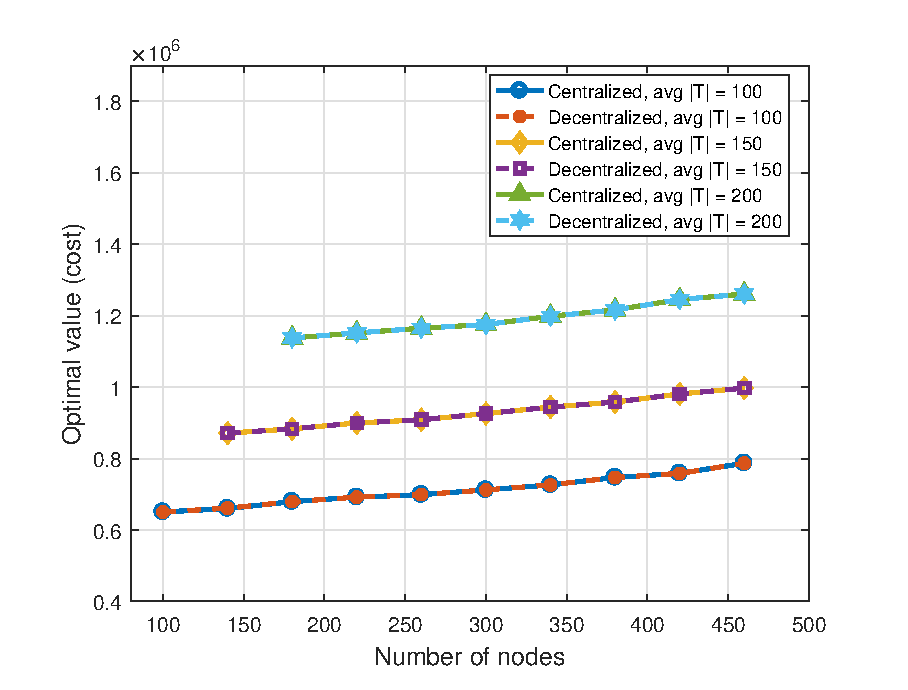
\includegraphics[width=12cm]{graphics/3-cent-decent/optimization_value_per_number_of_nodes}}
	\caption{مقدار تابع هدف(هزینه) دربرابر تعداد کل گره‌های موجود در شبکه برای دو روش متمرکز و غیرمتمرکز}
	\label{fig:optimization_value_per_number_of_nodes}
\end{figure}

    برای تاخیر مسیریاب‌ها فرض می‌کنیم که به صورت میانگین عبور بسته‌ها از مسیریاب‌های لایه 1، 2 میلی ثانیه، مسیریاب‌های لایه 2، 4 میلی ثانیه و مسیریاب‌های لایه 3، 10 میلی ثانیه طول می‌کشد.
\cref{fig:network} توپولوژی شبکه را که در شبیه‌سازی استفاده شده‌است نشان می‌دهد.

\begin{figure}[h!]
	\centerline{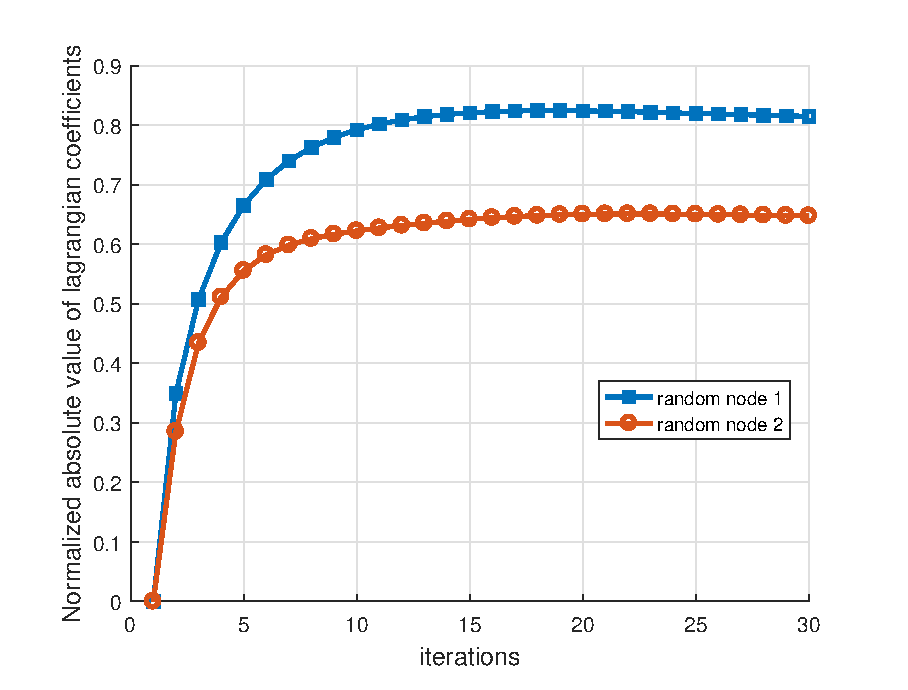
\includegraphics[width=12cm]{graphics/3-cent-decent/decentralized_lagrangian_coeffs_convergence}}
	\caption{نحوه‌ همگرا شدن اندازه ضرایب لاگرانژین در دو گره تصادفی در روش غیرمتمرکز}
	\label{fig:decentralized_lagrangian_coeffs_convergence}
\end{figure}

ظرفیت مربوط به هریک از گره‌ها به نجوی انتخاب شده است که بیشترین ظرفیت مربوط به گره‌های ابری و کمترین مربوط به گره‌های لبه باشد. که به ترتیب به نسبت اعداد 10، 9 و 8 درنظر گرفته شده است. حجم پردازنده مورد نیاز برای وظیفه‌ها نیز به صورت تصادفی اعداد حدود 40 واحد در نظر گرفته شده‌اند. حداقل زمان لازم جهت پردازش وظیفه‌ها به صورت تصادفی و حدود 15 میلی‌ثانیه فرض شده‌است. واحد قیمت پردازشی برای گره‌ها به صورتی در نظر گرفته شده است که ارزان‌ترین هزینه مربوط به گره‌های لایه ابری و گرانترین مربوط به گره‌‌های لایه لبه باشد، این اعداد به صورت تصادفی و به ترتیب به نسبت اعداد 1، 4 و 9 واحد در نظر گرفته شده‌است. نرخ پوآسون تولید وظیفه در گره‌های حسگری به صورت تصادفی و در حدود 50 واحد بر ثانیه برای هر وظیفه در هر گره حسگری درنظر گرفته شده‌است. 

\begin{figure}[h!]
	\centerline{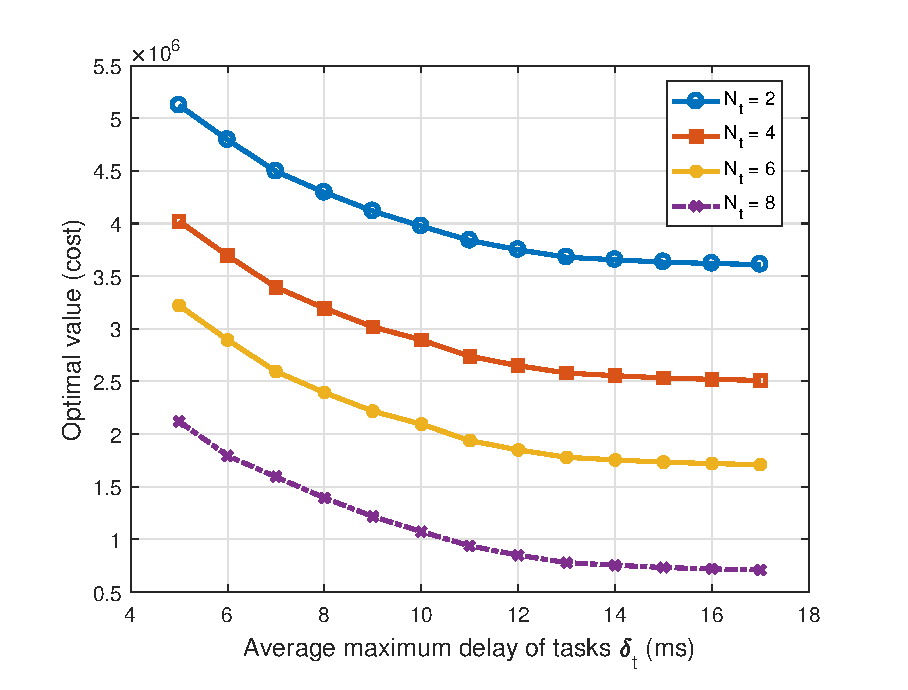
\includegraphics[width=12cm]{graphics/3-cent-decent/optimization_value_per_delay_for_dif_Nt}}
	\caption{مقدار تابع هدف(هزینه) دربرابر میانگین حداکثر تاخیر قابل قبول برای وظیفه‌ها $\delta_t$}
	\label{fig:optimization_value_per_delay_for_dif_Nt}
\end{figure}
	
	ابتدا لازم است که دقت دو روش متمرکز و غیرمتمرکز مقایسه شود. در \cref{fig:optimization_value_per_number_of_nodes} مقدار تابع هدف در این دو روش در برابر تعداد کل گره‌های موجود در شبکه از جمله گره‌های حسگری و گره‌های پردازشی دیده می‌شود. همانطور که دیده می‌شود این نمودار برای سه حالت مختلف از تعداد وظیفه‌ها رسم شده است و در هر سه حالت مقدار بهینه در روش متمرکز و غیرمتمرکز یکسان شده‌است. با افزایش تعداد کل وظیفه‌ها مقدار تابع هدف افزایش می‌یابد، همچنین با زیاد شدن کل گره‌های موجود در شبکه با فرض ثابت بودن تعداد وظیفه‌ها انتظار می‌رود که میزان تابع هدف تقریبا ثابت باشد، اما به دلیل اینکه با افزایش تعداد گره‌ها، تعداد گره‌های حسگری نیز افزایش می‌یابد، مقدار بهینه نیز اندکی افزایش می‌یابد. 

\begin{figure}[h!]
	\centerline{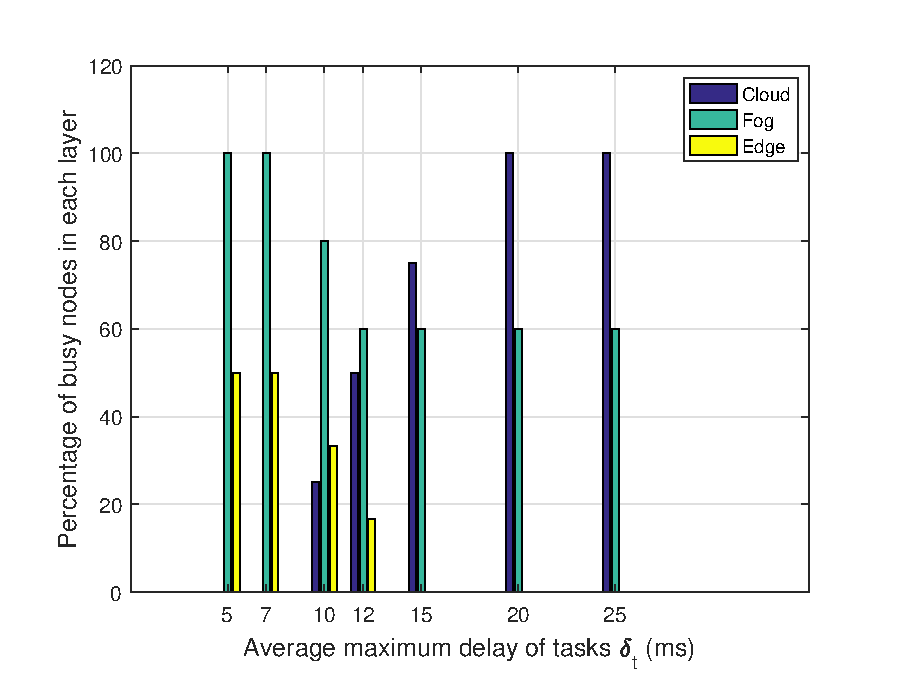
\includegraphics[width=12cm]{graphics/3-cent-decent/busynodes_per_delay}}
	\caption{درصد استفاده از گره‌های لایه‌های مختلف دربرابر میانگین حداکثر تاخیر قابل قبول برای وظیفه‌ها $\delta_t$}
	\label{fig:busynodes_per_delay}
\end{figure}

	درمورد روش غیرمتمرکز و نحوه‌ی همگرا شدن آن، دو گره به صورت تصادفی انتخاب شده‌است و در این دو گره مجموع اندازه‌ ضرایب لاگرانژ یعنی $\sqrt{|\eta_1|^2+|\eta_2|^2+|\nu_1|^2+|\nu_2|^2}$ به صورت یکه شده در طول زمان رسم شده است. در \cref{fig:decentralized_lagrangian_coeffs_convergence} می‌توانید این نتایج را ببینید.	

	در شبیه‌سازی بعدی تابع هدف براساس حداکثر تاخیرهای قابل قبول متفاوت برای وظیفه‌ها رسم شده است. با توجه به \cref{fig:optimization_value_per_delay_for_dif_Nt} می‌توان گفت که با افزایش میانگین حداکثر تاخیر قابل قبول برای وظیفه‌ها($\delta_t$) هزینه کل شبکه کاهش می‌یابد که دلیل این موضوع این است که استفاده از گره‌های ابری نسبت به گره‌های مه و لبه بیشتر می‌شود و از آنجایی که هزینه استفاده از گره‌های ابری کم‌تر است، هزینه کل شبکه کاهش می‌یابد. این نمودار برای چهار حالت مختلف از حداکثر تعداد قابل قبول برای تقسیم شدن وظیفه‌ها ($N_t$) رسم شده‌است. با توجه به \cref{fig:optimization_value_per_number_of_nodes} با کاهش $N_t$ این امکان کمتر می‌شود که وظیفه‌ها بین گره‌های مختلف شکسته شوند و هر وظیفه باید به صورت بخش‌های بزرگتری پردازش شود، درنتیجه استفاده از گره‌های مه و لبه بیشتر می‌شود و همین باعث می‌شود که هزینه کل شبکه بیشتر شود. 

\begin{figure}[h!]
	\centerline{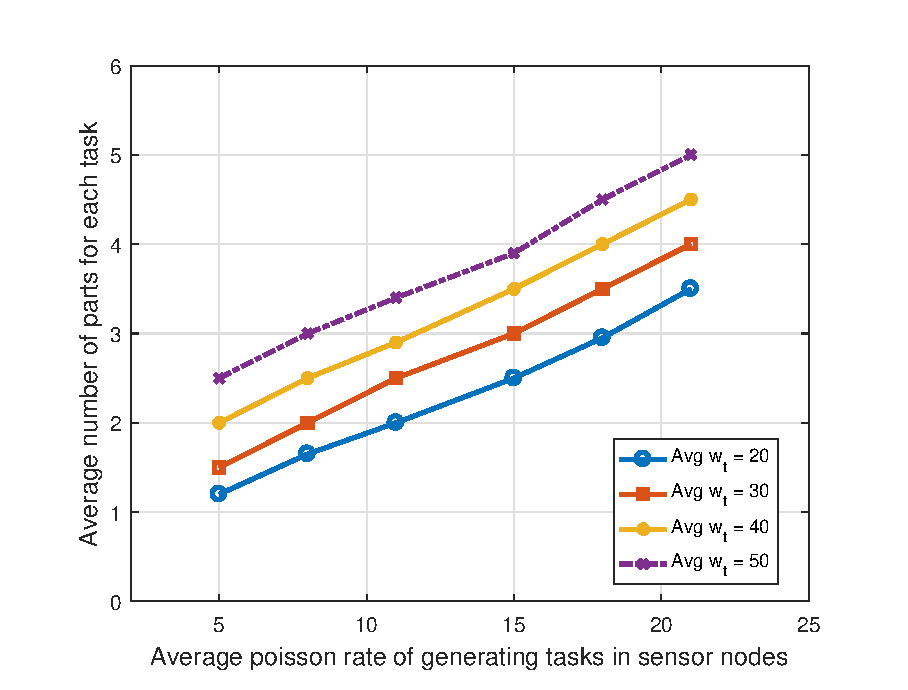
\includegraphics[width=12cm]{graphics/3-cent-decent/number_of_parts_per_task_generating_rate}}
	\caption{میانگین تعداد شکسته شدن وظیفه‌ها بین گره‌های مختلف دربرابر میانگین نرخ تولیدی وظیفه‌ها در گره‌های حسگری $\lambda_{t,s}$}
	\label{fig:number_of_parts_per_task_generating_rate}
\end{figure}

	در شبیه سازی بعدی میزان استفاده از گره‌های لایه‌های مختلف مورد تحلیل و بررسی قرار می‌گیرد. در \cref{fig:busynodes_per_delay} میانگین حداکثر تاخیر قابل قبول برای وظیفه‌ها در محور افقی قرار گرفته است و برای هر تاخیر، درصد استفاده از گره‌های هر لایه در محور عمودی نشان داده شده‌است. همانطور که دیده می‌شود با کاهش حداکثر میزان تاخیر قابل قبول لازم است که وظیفه‌ها بیشتر در سمت لبه پردازش شوند و این درصد استفاده از گره‌های این لایه را بیشتر می‌کند و بالعکس. 

	در آخرین شبیه‌سازی در این فصل قرار است که میزان شکسته‌شدن وظیفه‌ها بین گره‌های مختلف مورد بررسی قرار گیرد. برای این‌کار میزان نرخ تولید وظیفه‌ها در گره‌های حسگری تغییر کرده است و در هر مرحله میانگین تعداد شکسته شدن گره‌ها مورد بررسی قرار گرفته‌است. با توجه به \cref{fig:number_of_parts_per_task_generating_rate} می‌توان گفت که با افزایش میزان نرخ تولید وظیفه‌ها احتمال شکسته شدن وظیفه‌ها بین گره‌ها بیشتر می‌شود و میانگین تعداد تقسیم وظیفه‌ها افزایش می‌یابد. این نمودار برای میانگین حجم پردازشی وظیفه‌ها رسم شده‌است، که می‌توان گفت با افزایش میانگین حجم پردازشی، پردازش وظیفه‌ها سخت‌تر و درنتیجه میانگین تعداد تقسیم‌ها بیشتر می‌شود. 

	\section{جمع‌بندی و نتیجه‌گیری}
	در این فصل مدل سیستم برای مسئله تخصیص منابع پردازشی نوشته‌شد و مورد بررسی قرار گرفت. این مسئله غیرخطی بود که برای راحت‌تر شدن این مسئله خطی‌سازی شد. درادامه مسئله به کمک روش متمرکز حل شد و در نهایت یک الگوریتم برای حل مسئله به صورت غیرمتمرکز ارائه شد. هر دو روش گفته شده به جواب بهینه می‌رسند با این تفاوت که روش غیرمتمرکز در زمان خطی به جواب می‌رسد. 




\chapter{راه‌حل‌های اکتشافی و توزیع‌شده}\label{chap:4-heuristic_distributed}
\thispagestyle{empty}
\section{مقدمه}\label{subsection:inroduction_4}
	در \cref{chap:3-system_model_centralized_decentralized} مدل سیتم به‌صورت کامل توضیح داده شد، مسئله بهینه‌سازی تبیین شد و پس از خطی‌سازی، ابتدا به روش متمرکز و سپس در \cref{subsection:decentralized} به روش غیرمتمرکز بررسی و حل شد. 
	در این فصل قرار است دو راه‌حل دیگر برای مدل سیستم ارائه شده در \cref{chap:3-system_model_centralized_decentralized} ارائه شود. 
	 در قسمت اول قرار است یک راه‌حل توزیع‌شده مورد بررسی قرار می‌گیرد، این راه‌حل از مدل خطی‌شده در \cref{chap:3-system_model_centralized_decentralized} یعنی \cref{eqn:objective_func_final} استفاده می‌کند. این راه‌حل به صورت کاملا توزیع‌شده بین گره‌های شبکه و بدون نیاز به هیچ واحد سومی\LTRfootnote{Third-party} ارائه می‌شود.  
	 در قسمت بعد یک راه‌حل اکتشافی\LTRfootnote{Heuristic} ارائه و بررسی گردد، مزیت این راه‌حل این است که نیازی نیست مسئله به‌صورت خطی تبیین شود، اما عیب آن نسبت به دو راه‌حل ارائه شده در \cref{chap:3-system_model_centralized_decentralized} این است که این راه‌حل جواب زیربهینه\LTRfootnote{Sub-optimal} ارائه می‌دهد. 
	 این راه‌حل اکتشافی مبتنی بر یکی از الگوریتم‌های معروف به نام ویتربی\LTRfootnote{Viterbi} است، که در \cite{viterbi} تبیین شده است. 
	 
	 در ادامه این فصل، ابتدا راه‌حل توزیع‌شده\LTRfootnote{Distributed} مورد بررسی قرار می‌گیرد. 
	 سپس مقدمه‌ای در مورد الگوریتم ویتربی گفته می‌شود، سپس مسئله‌ بهینه‌سازی اصلی به‌صورتی‌که در این بخش قابل استفاده باشد بازنویسی می‌شود و درنهایت الگوریتم اکتشافی مربوطه ارائه می‌شود. در ادامه 
	درنهایت پس از بررسی همگرایی و پیچیدگی دو راه‌حل ارائه شده در این فصل، نتایج مربوط به این دو راه‌حل و همچنین در مقایسه با راه‌حل‌های ارائه‌شده در \cref{chap:3-system_model_centralized_decentralized} نمایش داده می‌شود و جمع‌بندی لازم ارائه می‌گردد. 
\section{راه‌حل توزیع‌شده}\label{subsection:distributed}

در این بخش قرار است یک راه‌حل دیگر برای حل مسئله اصلی خطی‌شده یعنی \cref{eqn:objective_func_final} ارائه شود. در این راه‌حل مسئله بهینه‌سازی به‌طور کامل شکسته می‌شود و به صورت توزیع‌شده حل می‌شود. برای این‌کار از الگوریتم ارائه شده در \cite{testa2019distributed} استفاده می‌شود. همانند راه‌حل‌های قبلی ابتدا مقدمه‌ای  در مورد این الگوریتم و نحوه‌ی کار کردن آن گفته می‌شود، سپس همین الگوریتم برای مسئله اصلی نوشته می‌شود و درنهایت نتایج شبیه‌سازی به نمایش گذاشته می‌شود. 
\subsection{الگوریتم توزیع‌شده}
فرض کنید که مسئله بهینه سازی خطی ترکیب عدد صحیح به صورت \cref{eqn:distributed:objective_func} باشد.
\begin{subequations}\label{eqn:distributed:objective_func}
	\begin{align}
		&\min_{z}c^Tz  \\
		&\text{\lr{subj. to}} \quad a_i^Tz \le b_i, i = 1, \dots, n  \\
		&z \in \mathbb{Z}^{d_Z} \times \mathbb{R}^{d_R} \\
		&d = d_Z + d_R  \\
		&a_i \in \mathbb{R}^d , b_i \in \mathbb{R}, c \in \mathbb{R}^d
	\end{align}
\end{subequations}
	همانطور که مشخص است متغیر اصلی مسئله یعنی $z$ از دو بخش گسسته و پیوسته تشکیل شده است و همچنین $n$ قید مختلف نیز وجود دارد. حال فرض کنید که شبکه‌ی گره‌ها شامل $N$ گره باشد و میخواهیم مسئله فوق را به صورت توزیع شده توسط این گره‌ها حل کنیم. می‌توان نشان داد که در صورتی که $n \ge N$ آن‌گاه این مسئله به جواب می‌رسد یعنی تعداد گره‌ها از تعداد قیدها بیشتر نباشد، دراین‌صورت می‌توان گفت که در هر گره حداقل یک قید بررسی می‌شود. در این صورت هر گره نیازی ندارد که در مورد قید یا قیدهای گره‌های دیگر چیزی بداند.
	گره‌های موجود در شبکه با یک گراف جهت‌دار کاملا متصل مدل‌سازی می‌شود. 
	
	در ادامه در مورد قیدهای موجود در مسئله \cref{eqn:distributed:objective_func} بیشتر صحبت خواهیم کرد، فرض کنید که کل قیدهای مسئله به صورت \cref{eqn:distributed:constraint_cont} نوشته شود با این تفاوت که متغیر اصلی مسئله کاملا پیوسته در نظر گرفته‌شود. همانطور که می‌دانیم شکل هندسی این قید در فضای پیوسه $d$ بعدی یک چندوجهی\LTRfootnote{Polyhedron} خواهد بود. حال اگر اشتراک این مجموعه و شرط گسسته بودن بعضی از اعضای متغیر اصلی را در نظر بگیریم آن‌گاه یک مجموعه جدید به نام $P_I$ شکل می‌گیرد که در \cref{eqn:distributed:constraint_int} نشان داده شده است. همانطور که می‌دانیم مجموعه $P_I$ لزوما محدب نخواهد بود در نتیجه مسئله بهینه‌سازی که بر روی این مجموعه تعریف می‌شود محدب نخواهد بود، لذا برای بررسی مسائلی که مجموعه قیدهای آن‌ها به صورت فوق باشد تلاش می‌شود به نجوی مجموعه قیدها محدب شود که بتوان از مزیت‌های مربوط به مسائل بهینه‌سازی محدب استفاده برد. برای این‌کار معمولا از مفهوم پوش محدب\LTRfootnote{Convex  hull} استفاده می‌شود. در \cref{fig:distributed:polyhedron} یک مثال از چندوجهی و پوش محدب آورده شده است. 
	
\begin{align}
	&P := \bigcap_{i=1}^n \{ z \in \mathbb{R}^d : a_i^Tz \le b_i\} \label{eqn:distributed:constraint_cont} \\
	&P_I = P \cap \{\mathbb{Z}^{d_Z} \times \mathbb{R}^{d_R}\} \label{eqn:distributed:constraint_int}
\end{align}	

\begin{figure}[h]
	\centerline{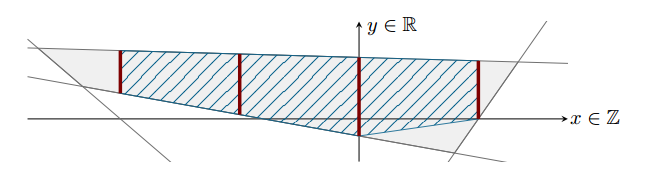
\includegraphics[width=15cm]{graphics/4-heuristic-dist/polyhedron}}
	\caption{مثالی از چند وجهی $P$ که قسمت خاکستری رنگ است و همچنین مجموعه قابل قبول جواب مسئله یعنی $P_I$ که با خطوط پررنگ قرمز مشخص شده است و مجموعه پوش محدب از جواب قابل قبول یعنی \lr{conv$(P_I)$} که ناحیه هاشور خورده آبی رنگ است. فضای استفاده شده به صورت دو بعدی است.}
	\label{fig:distributed:polyhedron}
\end{figure}
	باتوجه به نکات گفته‌شده یک مسئله خطی پیوسته در \cref{eqn:distributed:objective_func_linear} معرفی می‌کنیم که جواب بهینه‌ این مسئله با جواب بهینه مسئله \cref{eqn:distributed:objective_func} یکسان خواهد بود. به صورت شهودی با توجه به \cref{fig:distributed:polyhedron} می‌توان گفت که جواب یک مسئله بهینه‌سازی خطی در گوشه‌های منطقه‌ قابل‌قبول\LTRfootnote{Feasible region} آن خواهد بود. بنابراین نقطه بهینه\LTRfootnote{Optimal point} در این دو مسئله یکسان خواهد بود. 
%\begin{subequations}\label{eqn:distributed:objective_func_linear}
	\begin{align}\label{eqn:distributed:objective_func_linear}
	&\min_{z}c^Tz \notag \\
	&\text{\lr{subj. to}} \quad z \in \text{\lr{conv}}(P_I) \notag \\
	&z \in \mathbb{R}^d
	\end{align}
%\end{subequations}
%todo fesible region ltrfoot
	با توجه به آن‌چه گفته شد از این ایده برای حل کردن مسائل بهینه‌سازی خطی ترکیب عدد صحیح می‌توان استفاده کرد، به این صورت که ابتدا مسئله را به صورت خطی پیوسته در نظر می‌گیرند و هر بار یک قید جدید به مسئله اضافه می‌کنند به صورتی که فضای قابل قبول برای مسئله کوچک و کوچک‌تر شود و در نهایت با شروع از $P$ به \lr{conv$(P_I)$} می‌رسند. 
	
	در ادامه نحوه‌ی عملکرد این دسته از الگوریتم ها که به الگوریتم‌های صفحه برش\LTRfootnote{Cutting-plane} معروف هستند به صورت کلی آورده می‌شود. 
\begin{latin}
	\begin{algorithm}
		\caption{Centralized Cutting-Plane Meta-Algorithm}
		\label{alg:distributed:centralized}
		\begin{algorithmic}[1]
			\State Initialization: $ P := \bigcap_{i=1}^n \{ z \in \mathbb{R}^d : a_i^Tz \le b_i\}$
			\State LP solver: Find an optimal solution $z^{LP} = (x^{LP},y^{LP})$ of the LP relaxation of \cref{eqn:distributed:objective_func} with polyhedron P. \label{eqn:alg_steps:distributed_centralized_lp_solver}
			\State Check feasibility: if $x^{LP} \in \mathbb{Z}^{d_Z}$, go to \cref{eqn:alg_steps:distributed_centralized_last}.
			\State Cutting-Plane: $h = CUTORACLE(z^{LP},P,c)$.
			\State Update: $P := P \cap h$ and go to \cref{eqn:alg_steps:distributed_centralized_lp_solver}.
			\State Output: $z^{LP}$\label{eqn:alg_steps:distributed_centralized_last}.
		\end{algorithmic}
	\end{algorithm}
\end{latin}

	در \cref{alg:distributed:centralized} از مفهوم $CUTORACLE$ استفاده شده‌است که نشان‌دهنده یک تابع است که باتوجه به نقطه بهینه فعلی و آخرین چندوجهی مربوط به قیدها، یک قید جدید تولید می‌کند به‌طوریکه اشتراک چندوجهی قبلی و این قید جدید شامل پوش محدب مجموعه گسسته \lr{conv$(P_I)$} باشد اما شامل اخرین نقطه بهینه $z^{LP} = (x^{LP},y^{LP})$ نباشد.
	
	در ادامه لازم است که چند مفهوم دیگر تعریف شود. یک جعبه محدود به صورت \cref{eqn:distributed:bounding_box} تعریف می‌شود که در ادامه از آن استفاده خواهد شد. فرض می‌شود که $P \subset H_M$.
\begin{equation}\label{eqn:distributed:bounding_box}
H_M := \bigcap_{l=1}^d (\{ z_l \le M \} \cap \{ z_l \ge -M \})
\end{equation}
	یک مفهوم دیگر به نام پایه\LTRfootnote{Basis} تعریف می‌شود، فرض کنید که یک مسئله بهینه‌سازی خطی پیوسته با مجموعه قید $P := \bigcap_{i=1}^n P_i$ داریم که هریک از $P_i$ ها یک نیم‌فضا\LTRfootnote{Half-spce} است، پایه $B$ مجموعه‌ تشکیل شده از تقاطع حداقل تعداد نیم‌فضا $P_{l_1}, \dots, P_{l_q}$ است به صورتی‌که $q \le d$ و جواب بهینه مسئله بهینه سازی بر روی مجموعه قید $P$ با جواب همان مسئله بر روی مجموعه قید $B$ برابر است. اگر برای حل کردن مسئله بهینه‌سازی از الگوریتم $LEXOPTIMAL$ که نوعی الگوریتم سیمپلکس\LTRfootnote{Simplex} است استفاده شود، می‌توان نشان داد که $B$ دقیقا از تقاطع $d$ نیم‌فضا تشکیل می‌شود.  الگوریتم $LEXOPTIMAL$ به تفصیل در \cite{jones2007lexicographic} توضیح داده شده‌است.
	%todo lexoptimal cite
	
\begin{latin}
	\begin{algorithm}
		\caption{Distributed Meta-Algorithm}
		\label{alg:distributed:int_distributed}
		\begin{algorithmic}[1]
			\Statex State $(z^{[i]},B^{[i]})$
			\Statex Initializing    
			\State $h^{[i]} = h_{i0} \cap H_M$
			\State $(z^{[i]},B^{[i]}) = LPLEXSOLV(h^{[i]}, c)$
			\Statex Evolution 
			\State $(h_{MIG}(t),h_c(t)) = CUTORACLE(z^{[i]}(t),B^{[i]}(t),c)$
			\State $\displaystyle H_{TMP}(t) = (\bigcap_{j \in N_i(t)}B^{[j]}(t)) \cap B^{[i]}(t) \cap h^{[i]} \cap h_{MIG}(t) \cap h_c(t)$
			\State $(z^{[i]}(t+1),B^{[i]}(t+1)) = LPLEXSOLV(H_{TMP}, c)$
		\end{algorithmic}
	\end{algorithm}
\end{latin}
%todo h_mig H_M
در \cref{alg:distributed:int_distributed} خروجی تابع CUTORACLE به‌صورت دو قسمتی است. که لازم است در مورد آن صحبت شود. در \cite{gomory1960algorithm} یک روش برش به نام MIG\LTRfootnote{Mixed-Integer Gomory} ارائه شده است و اثبات شده است که در صورتی‌که تابع هدف مسئله بهینه‌سازی به صورت گسسته باشد، این روش صفحه برش می‌تواند مسئله را حل کند. خروجی تابع که به صورت $h_{MIG}$ نشان داده شده‌است، مربوط به این نحوه‌ی برش می‌باشد. خروجی دیگر که با نماد $h_c$ نشان داده شده‌است در \cref{eqn:distributed:cost_based_cut} آورده شده‌است. 
\begin{align}\label{eqn:distributed:cost_based_cut}
	h_c = \{ c^Tz > \lceil c^Tz^{LP}\rceil \}	
\end{align}
	بنابراین از \cref{alg:distributed:int_distributed} برای حل کردن مسئله خطی ترکیب عددصحیح به‌صورت کاملا توزیع‌شده استفاده می‌شود. نحوه کار این الگوریتم بدین صورت است ابتدا هریک از گره‌های موجود در شبکه یک یا چند قید اختصاصی برای شروع دارد. در اولین مرحله هر گره مسئله خطی معادل را با توجه به قیدهای اولیه حل می‌کند و برش‌ها و مجموعه پایه متناسب را می‌سازد. در هر مرحله هر گره پایه تولیدی همسایه‌هایش را دریافت می‌کند و با اخرین پایه و برش‌های تولیدی خودش اشتراک می‌گیرد و در مرحله بعد از این پایه برای حل مسئله خطی معادل استفاده می‌کند. برای کارکرد درست الگوریتم این شرط اساسی وجود دارد که تابع هدف مسئله بهینه‌سازی به صورت گسسته (عددصحیح) باشد. 
	برای حل مشکل شرط گسسته بودن تابع هدف یک الگوریتم دیگر ارائه می‌شود که در \cref{alg:distributed:epsilon_distributed} آورده شده‌است. ابتدا مسئله اصلی نوشته شده در \cref{eqn:distributed:objective_func} به صورت \cref{eqn:distributed:objective_func_epigraph} بازنویسی می‌شود، که مدل epigraph نامیده می‌شود. 
	\begin{subequations}\label{eqn:distributed:objective_func_epigraph}
		\begin{align}
		&\min_{\rho,z}\rho \\
		&\text{\lr{subj. to}} \quad a_i^Tz \le b_i, i = 1, \dots, n  \\
		&c^Tz \le \rho \\
		&\rho \in \mathbb{R}, z \in \mathbb{Z}^{d_Z} \times \mathbb{R}^{d_R} \\
		\end{align}
	\end{subequations}
	می‌دانیم که $\rho$ لزوما به صورت عددصحیح نیست، بنابراین یک متغیر دیگر به نام $\rho_I$ که فرض می‌کنیم به صورت عددصحیح است، به‌صورت $\epsilon\rho_I = \rho$ تعریف می‌شود که $\epsilon$ یک عدد مثبت کوچک است. حال مسئله بهینه‌سازی مجددا به فرم \cref{eqn:distributed:objective_func_epigraph_int} بازنویسی می‌شود و درنهایت الگوریتم توزیع‌شده برای این مسئله نوشته می‌شود. 
	\begin{subequations}\label{eqn:distributed:objective_func_epigraph_int}
		\begin{align}
		&\min_{\rho_I,z}\rho_I \\
		&\text{\lr{subj. to}} \quad a_i^Tz \le b_i, i = 1, \dots, n  \\
		&c^Tz \le \epsilon \rho_I \\
		&\rho_I \in \mathbb{Z}, z \in \mathbb{Z}^{d_Z} \times \mathbb{R}^{d_R}, \epsilon > 0 \\
		\end{align}
	\end{subequations}
	درنهایت می‌توان \cref{alg:distributed:epsilon_distributed} را به‌صورت زیر نوشت که برای تمام مسئله‌های خطی ترکیب عددصحیح جواب می‌دهد. توضیح بیشتر درمورد جزئیات این الگوریتم این‌که هریک از گره‌ها قید اولیه و محلی خود را به صورت $h_{i0} = \{ a_i^Tz \le b_i\} \cap \{c^Tz \le \epsilon\rho\}$ در نظر می‌گیرد. زوج متغیر $\rho_I$ , $z$ را نیز به عنوان هزینه جدید درنظر می‌گیریم و با $e_1$ نشان می‌دهیم. 
\begin{latin}
	\begin{algorithm}
		\caption{Distributed Algorithm}
		\label{alg:distributed:epsilon_distributed}
		\begin{algorithmic}[1]
			\Statex State $((\rho_I^{[i]},z^{[i]}),B^{[i]})$
			\Statex Initializing    
			\State $h^{[i]} = h_{i0} \cap H_M$
			\State $((\rho_I^{[i]},z^{[i]}),B^{[i]}) = LPLEXSOLV(h^{[i]}, e_1)$
			\Statex Evolution 
			\State $h_{MIG}(t) = MIGORACLE((\rho_I^{[i]}(t),z^{[i]}(t)),B^{[i]}(t),c)$
			\State $h_c(t) = \{ \rho_I \ge \lceil\rho_I^{[i]}(t)\rceil \} $
			\State $\displaystyle H_{TMP}(t) = (\bigcap_{j \in N_i(t)}B^{[j]}(t)) \cap B^{[i]}(t) \cap h^{[i]} \cap h_{MIG}(t) \cap h_c(t)$
			\State $((\rho_I^{[i]}(t+1),z^{[i]}(t+1)),B^{[i]}(t+1)) = LPLEXSOLV(H_{TMP}, e_1)$
		\end{algorithmic}
	\end{algorithm}
\end{latin}

در هر دو الگوریتم توزیع‌شده ارائه شده، هر گره متغیر اصلی مسئله را به صورت محلی ذخیره می‌کند و در هر مرحله بعد از تبادل اطلاعات با همسایه‌های خود و دریافت قید(پایه)های جدید، متغیر اصلی مسئله را بروز رسانی می‌کند. سوالی که پیش می‌آید، این است که هر گره چگونه بداند فرآیند حل مسئله به اتمام رسیده است یا نه، در \cite{testa2019distributed} گفته شده‌است که هروقت یک گره از همسایه‌های خود هیچ قید جدیدی دریافت نکرد، می‌توان گفت که فرآیند حل مسئله به پایان رسیده است. 

	در این قسمت لازم است که مسئله مربوط به این پایان‌نامه را به فرم \cref{eqn:distributed:objective_func} و سپس \cref{eqn:distributed:objective_func_epigraph} بنویسم. ابتدا لازم است که متغیر اصلی یعنی $z$ را تعریف کنیم، که در \cref{eqn:distributed:def_z} انجام شده‌است. در این رابطه ابتدا کلیه متغیرهای گسسته (دودویی) مسئله یعنی $x$  و سپس متغیرهای پیوسته یعنی $\beta$ به صورت یک بردار در کنار هم قرار داده می‌شود. در \cref{eqn:distributed:def_z} جهت نمایش درست از قراردادهای استاندارد نرم‌افزار متلب\LTRfootnote{Matlab} استفاده شده‌است. 
	
\begin{subequations}\label{eqn:distributed:def_z}
	\begin{align}
		&z = (\underline{x_e}^T, \underline{x_f}^T, \underline{x_c}^T, 
		\underline{\psi_e}^T, \underline{\psi_f}^T, \underline{\psi_c}^T,
		\underline{\underline{\beta_{e}}}(:)^T, \underline{\underline{\beta_{f}}}(:)^T, \underline{\underline{\beta_{c}}}(:)^T)^T \\
		&\underline{x_e} = (x_{e,1}, \dots, x_{e,|T|})^T \\
		&[\underline{\underline{\beta_{e}}}]^i_j = \beta_{i,j,e}
	\end{align}
\end{subequations}
%todo matrix elements syntax and all elements of a matrix in a row syntax
در قدم بعدی لازم است که قیدها را بین گره‌ها تقسیم کنیم، در مورد قیدهایی که تفکیک‌پذیر هستند، یعنی قیدهای \cref{eqn:constraint_load_conservation_computing_nodes}، \cref{eqn:constraint_request_flow_existence}،\cref{eqn:constraint_psi} ، \cref{eqn:constraint_load_managing_linear}، \cref{eqn:constraint_delay_linear} و \cref{eqn:constraint_queue_stability_linear} وضعیت مشخص است و هر گره قید مختص به خود را دارد، اما در مورد دو قید \cref{eqn:constraint_scalability_coupling} و \cref{eqn:constraint_load_conservation_sensor_nodes_coupling_new2} که به صورت مشترک هستند لازم است تصمیم گرفته‌شود. تعداد قیدهای دسته اول $|T|$ است و تعداد قیدهای دسته دوم $|T| \times |S|$ است، در حالی‌که تعداد گره‌های پردازشی از \cref{eqn:def_globals} $l$ است. حال لازم است که این دودسته قید بین گره‌ها توزیع شوند، برای توزیع بهتر می‌توان از این ایده کمک گرفت که توزیع قیدها را از گره‌هایی که توانایی پردازش بیشتری دارند شروع کرد. به‌صورت میانگین به هر گره $\frac{|T|\times(|S|+1)}{l}$ قید می‌رسد. در نهایت $c$ به راحتی با مقایسه با تابع هدف در \cref{eqn:objective_func_final} قابل استخراج است. 

\section{مقدمه‌ای بر ویتربی}
در این بخش ابتدا لازم است که در مورد الگوریتم ویتربی و نحوه‌ی کار آن صحبت شود. این الگوریتم یک الگوریتم پویا\LTRfootnote{Dynamic}، برای پیدا کردن محتمل‌ترین مسیر از حالت‌های پنهان، با داشتن یک توالی از مشاهدات است. این الگوریتم اغلب در مواردی به‌کار می‌رود که با داشتن یک مدل پنهان مارکف و توالی‌ از مشاهدات، می‌خواهیم بدانیم چه توالی‌ از حالت‌ها (مسیر) این مشاهدات را تولید کرده‌اند. به عبارت دیگر ما به‌دنبال محتمل‌ترین مسیر به‌وجودآورنده مشاهدات در یک مدل پنهان مارکف هستیم. 

به عنوان ابتدایی‌ترین پاسخ می‌توانیم تمامی مسیرهای ممکن که مشاهده ما را تولید می‌کنند، پیدا کنیم، سپس با محاسبه احتمال آنها، محتمل‌ترین مسیر را بدست آوریم اما می‌توان نشان داد که پیچیدگی زمانی این راه‌حل نسبت به طول توالی $n$، از اندازه نمایی $(O(a^n))$ است. الگوریتم ویتربی یک راه‌حل ارائه می‌دهد که هزینه محاسباتی آن به صورت خطی با طول توالی افزایش می‌یابد، اصطلاحا هزینه آن از اندازه چندجمله‌ای است. فرم نهایی مسئله را می‌توان بدین صورت نوشت: می‌خواهیم مسیر بهینه‌ای مانند $\displaystyle \pi^* = \arg \max_\pi P(x,\pi)$ داشته باشیم، که در آن $x=(x_1, \dots, x_L)$ یکه توالی از مشاهدات و $\pi = (\pi_1, \dots, \pi_L)$ یک توالی از متغیرهای پنهان باشد. 

نحوه‌ی عملکرد این الگوریتم بدین صورت است که مسئله را به صورت یک گراف چندمرحله‌ای\LTRfootnote{Multistage} در نظر می‌گیرد. تعداد مرحله‌\LTRfootnote{Stage}ها برابر است با تعداد مشاهدات و در هر مرحله یکی از مشاهدات مورد بررسی قرار می‌گیرد. در هر مرحله تعدادی حالت\LTRfootnote{State} درنظر گرفته‌می‌شود که هر حالت یک پیشامد ممکن در آن مرحله را بیان می‌کند. حال لازم است که دو مدل تابع هزینه\LTRfootnote{Cost function} تعریف شود یک تابع به عنوان هزینه‌ی بودن در هر حالت در هر مرحله و یک تابع به عنوان هزینه انتقال از یک حالت در یک مرحله به یک حالت دیگر در مرحله بعد است، در واقع این دوتابع به نحوی باید مکمل یکدیگر باشند. در هر مرحله، برای هریک از حالت‌های آن مرحله یک مسیر به عنوان مسیر نجات‌یافته\LTRfootnote{Survived path} تعریف می‌شود که برابر است با مسیری از اولین مرحله تا مرحله فعلی که کمترین هزینه ممکن را دارد. در آخرین مرحله نیز هریک از حالت‌ها یک مسیر نجات‌یافته دارد، در این مرحله حالتی که کمترین هزینه ممکن را دارد، مسیر نجات‌یافته‌اش به عنوان مسیر ویتربی\LTRfootnote{Viterbi path} مشخص می‌شود که این مسیر درواقع پاسخ مسئله است. 
%todo a picture about viterbi
\section{راه‌حل اکتشافی مبتی بر ویتربی (VTP)}	\label{subsection:vtp}
در این بخش قرار است باتوجه به مقدمه‌ی گفته شده متغیرهای مربوط به الگوریتم ویتربی را برای مسئله اصلی تعریف کنیم. 
ابتدا صورت مسئله اصلی که به صورت غیرخطی است در \cref{eqn:heuristic:def_optimization_problem} آورده می‌شود. 
\begin{align}\label{eqn:heuristic:def_optimization_problem}
	& \min \sum_{t \in T}\sum_{e \in E} K_1\pi_ex_{t,e}\lambda_{t,e} + K_2\pi_ex_{t,e} \notag \\
	& + \sum_{t \in T}\sum_{f \in F} K_1\pi_fx_{t,f}\lambda_{t,f} + K_2\pi_fx_{t,f} \notag \\
	& + \sum_{t \in T}\sum_{c \in C} K_1\pi_cx_{t,c}\lambda_{t,c} + K_2\pi_cx_{t,c} \notag \\
	&\text{\lr{subj. to}}  %todo edit subj to
	\cref{eqn:constraint_load_conservation_computing_nodes}
	\cref{eqn:constraint_request_flow_existence}
	\cref{eqn:constraint_load_managing}\notag \\
	&\cref{eqn:constraint_delay}
	\cref{eqn:constraint_queue_stability}
	\cref{eqn:constraint_load_conservation_sensor_nodes_coupling}
	\cref{eqn:constraint_scalability_coupling}
\end{align}
حال لازم است که متغیرهای مربوط به الگوریتم ویتربی متناسب با مسئله‌ ما تعریف شوند، می دانیم که هدف از مسئله ما این است که تعدادی وظیفه به تعدادی گره پردازشی ارسال شوند؛ درواقع قرار است هرکدام از این وظیفه‌ها در یک یا چند گره پردازشی، پردازش شوند، با این هدف که کل هزینه موجود در شبکه کمترین مقدار ممکن باشد. حال می‌توانیم اینگونه فرض کنیم که هر وظیفه یک مشاهده است و هر گره پردازشی نیز یک پیشامد است یعنی هر وظیفه را به عنوان یک مرحله در نظر بگیریم و در هر مرحله، هر حالت برابر است با یک گره پردازشی، پس درواقع با توجه به \cref{eqn:def_globals} $l$ حالت مختلف داریم. در نهایت الگوریتم ویتربی باید طوری طراحی شود که مسیر ویتربی نشان‌دهنده این باشد که هر وظیفه در کدام گره پردازش شود یا درواقع مسیر ویتربی کمترین هزینه موجود در شبکه را نشان دهد.
نکته‌ای که باید مدنظر قرار بگیرد قابلیت پردازش یک وظیفه در چند گره است، همانطور که قبلا توضیح داده شد، این قابلیت بدین صورت است که هر وظیفه این امکان را دارد که شکسته شود و در دو یا چند گره پردازشی پردازش شود و حداکثر می‌تواند در $N_t$ گره پردازش شود. 
برای اضافه شدن این قابلیت به الگوریتم مربوطه، در تعداد مرحله‌های الگوریتم یک تغییر کوچک ایجاد می‌کینم به‌این‌صورت که به‌جای اینکه هر وظیفه را یک مرحله در نظر بگیریم، هر بخش شکسته‌شده از هر وظیفه را یک مرحله درنظر می‌گیریم، پس در نهایت $ \displaystyle L_V=\sum_{t \in T} N_t$ مرحله خواهیم داشت. 
برای حالت‌های هر مرحله نیز لازم است که یک تغییر کوچک ایجاد شود؛ برای هر وظیفه در بخش اول، حالت‌های ممکن برابر است با همان حالت‌های قبل یعنی $l$ حالت، اما در مورد بخش‌های بعدی یک حالت دیگر که حالت صفر $(0)$ نام دارد درنظر گرفته‌می‌شود. تعداد حالت‌های ممکن باتوجه به شماره‌ی مرحله در \cref{eqn:heuristic:def_states} دیده می‌شود. 
\begin{subequations}\label{eqn:heuristic:def_states}
	\begin{align}
		&Z_n =
		\begin{cases}
			\{0\} \bigcup S, & \text{$u = (n \mod N_t) = 1$} \\
			S,               & \text{در غیر این‌صورت}
		\end{cases}
		,n = 1, \dots, L_V \\
		&S = E \cup F \cup C
	\end{align}
\end{subequations}
بنابراین تا اینجای کار تعداد مرحله‌ها و همچنین حالت‌های هر مرحله مشخص شد. در ادامه لازم است که چند تابع مختلف تعریف شود یکی از آن‌ها تابع هزینه انتقال از یک حالت در یک مرحله به یک حالت دیگر در مرحله بعد است، که به صورت \cref{eqn:heuristic:def_tx_cost} تعریف می‌شود. 
\begin{subequations}
	\begin{align}\label{eqn:heuristic:def_tx_cost}
		&\Theta_{n-1,n}^{i,j} = \Gamma_{t,u,j} + \phi_{n-1}^i \\
		&u \in \{1, \dots, N_t\}
	\end{align}
\end{subequations}
در \cref{eqn:heuristic:def_tx_cost}، $n$ نشان‌دهنده‌ی مرحله، $t$ نشان دهنده وظیفه و $u$ نشان‌دهنده‌ی شماره‌ی بخش مربوط به هر وظیفه است که درواقع برای وظیفه $t$ عددی است بین یک تا $N_t$. $i$ و $j$ نشان‌دهنده‌ی حالت هستند. همچنین $\phi_{n-1}^i$ هزینه‌ی بودن در مرحله $n-1$ و حالت $i$ است. متغیر $\Gamma$ در \cref{eqn:def_Gamma} تعریف شده است. 

در ادامه یک متغیر دیگر به نام $T_{n-1,n}^{i,j}$ تعریف می‌کنیم که نشان‌دهنده‌ی تاخیر سیستم برای زمانی است که وظیفه مورد نظر در گره $j$ پردازش شود و الگوریتم ویتربی از حالت $i$ در مرحله قبل به این حالت بیاید. این متغیر در \cref{eqn:heuristic:def_delay_level} تعریف شده‌است. 
\begin{align}\label{eqn:heuristic:def_delay_level}
	T_{n-1,n}^{i,j} =
	\begin{cases}
		0,				& \text{$j = 0$} \\
		\tau_{t,u,j},  	& \text{در غیر این‌صورت}
	\end{cases}
	,n = 1, \dots, L_V
\end{align}
در معادله بالا بعد از مشخص شدن وظیفه و گره پردازشی $\tau$ را به راحتی می‌توان به کمک \cref{eqn:def_delay_final} محاسبه کرد. تنها قسمتی که لازم است در مورد آن صحبت شود مقدار $\lambda$ در \cref{eqn:def_delay_final} است. برای هر وظیفه نرخ کل جریان تولیدی در حسگرها مقداری مشخص است که لازم است در طی حل مسئله کل این نرخ تولیدی برای پردازش به گره‌های پردازشی برسد؛ پس در هر مرحله از الگوریتم لازم است مشخص شود چه حجمی از کل جریان تولیدی مورد بررسی قرار می‌گیرد. ایده‌ی به کار رفته در الگوریتم به این صورت است که ابتدا فرض می‌شود کل جریان تولیدیِ مربوط به هر وظیفه در مرحله مربوط به بخش اول از آن وظیفه درنظر گرفته می‌شود، در صورتیکه در یک مرحله هیچ گره‌ای پیدا نشود که منبع کافی برای پردازش کامل وظیفه را داشته باشد، آنگاه وظیفه شکسته می‌شود، یعنی بخشی از جریان تولیدی برای بخش‌های بعدی در نظر گرفته می‌شود و الگوریتم از بخش اولِ آن وظیفه دوباره اجرا می‌شود. جزئیات دقیق‌تری درمورد آن‌چه که گفته شد در \cref{alg:heuristic} آمده‌است. 

حال با توجه به متغیرهای تعریف شده برای هر حالت در هر مرحله می‌توان مسیر نجات‌یافته را به صورت \cref{eqn:heuristic:def_survived_path} پیدا کرد. 
\begin{align}\label{eqn:heuristic:def_survived_path}
	&I_n^j = \arg \min_{i \in XP_n^j} (D_{n-1,n}^{i,j}) \\
	&D_{n-1,n}^{i,j} = \Theta_{n-1,n}^{i,j} + M_k \times (T_{n-1,n}^{i,j} - OD_n^j) \times I(T_{n-1,n}^{i,j} - OD_n^j) \notag \\
	&+M_k \times (\lambda_{t,u,j} - \mu_{t,u,j}) \times I(\lambda_{t,u,j} - \mu_{t,u,j})
\end{align}	
در \cref{eqn:heuristic:def_survived_path} $D_{n-1,n}^{i,j}$ به عنوان معیار نهایی تصمیم‌گیری برای انتخاب مسیر بین حالت $i$ از مرحله $n-1$ و حالت $j$ از مرحله $n$ درنظر گرفته می‌شود. $I_n^j$ به عنوان شمارنده مسیرنجات‌یافته و $XP_n^j$ به عنوان مجموعه‌ی حالت‌های ممکن از مرحله $n-1$ که منابع کافی جهت ورود به حالت $j$ را دارند، درنظر گرفته‌می‌شود. می‌توان گفت که $XP_n^j \subset Z_{n-1}$، یعنی گره‌هایی که منبع کافی جهت انتقال به حالت جدید را ندارند از کل مجموعه حالت‌های مرحله قبل حذف می‌شوند. $M_k$ به عنوان یک هزینه سنگین در نظر گرفته می‌شود برای حالت‌هایی که تاخیر پردازش در آن‌ها از حداقل تاخیر قابل قبول برای پردازش وظیفه بیشتر است. یک متغیر دیگر به‌نام $OD_n^j$ دیده‌می‌شود، که می‌توان گفت بیانگر تاخیر درخواستی\LTRfootnote{Ordinary delay} برای وظیفه موردنظر است که در \cref{eqn:heuristic:def_ordinary_delay} آورده شده است در این رابطه این تاخیر برابر با میزان تاخیر درخواستی هر وظیفه درنظر گرفته‌شده‌است، درحالیکه می‌توانیم برای اطمینان بیشتر این تاخیر را اندکی کمتر از تاخیر درخواستی وظیفه در آن مرحله در نظر بگیریم که از همگرا شدن الگوریتم اطمینان بیشتری حاصل کنیم. قید مربوط به پایداری صف در گره‌ها نیز در این عبارت گنجانده شده است، به صورتی‌که اگر در یک حالت از یک مرحله مقدار متغیرها به‌گونه‌ای باشد که باعث شود صف موجود در گره ناپایدار شود، برای ورود به آن حالت هزینه زیادی درنظر گرفته می‌شود.

\begin{align}\label{eqn:heuristic:def_ordinary_delay}
	OD_n^j = 
	\begin{cases}
		\infty, & \text{$j = 0$} \\
		\delta_t,& \text{در غیر این‌صورت}
	\end{cases}
\end{align}
در هر مرحله از الگوریتم لازم است که مسیر نجات‌یافته را برای هر حالت ذخیره کنیم برای این کار از یک بردار به نام $\Lambda$ استفاده می‌کنیم، که به صورت \cref{eqn:heuristic:def_Lambda} بروزرسانی می‌شود. 
\begin{align}\label{eqn:heuristic:def_Lambda}
	\Lambda_n^j[u] = 
	\begin{cases}
		\Lambda_n^{I_n^j}[u], & 1 \le u \le n-1 \\
		j, 				& u = n
	\end{cases}
\end{align}
عملکرد \cref{eqn:heuristic:def_Lambda} بدین صورت است که در هر حالت پس از مشخص شدن شمارنده مربوط به حالت نجات یافته، مسیر نجات‌یافته برای حالت فعلی برابر است به مسیر نجات‌یافته برای حالت نجات‌یافته، به اضافه‌ی خود حالت فعلی. 
\begin{figure*}[!t]
	\resizebox{1 \textwidth}{!}{%
		\begin{tikzpicture}[scale=1, every node/.style={scale=0.8}]
			\draw (2,6) circle (0.5cm);
			\draw (2,8) circle (0.5cm);
			\draw (2,10) circle (0.5cm); %%4.2800    6.5600    8.8400   11.1200   13.4000   15.6800   17.9600
			
			\draw (4.28,4) circle (0.5cm);
			\draw (4.28,6) circle (0.5cm);
			\draw (4.28,8) circle (0.5cm);
			\draw (4.28,10) circle (0.5cm);
			
			\draw (6.56,6) circle (0.5cm);
			\draw (6.56,8) circle (0.5cm);
			\draw (6.56,10) circle (0.5cm);
			
			\draw (8.84,4) circle (0.5cm);
			\draw (8.84,6) circle (0.5cm);
			\draw (8.84,8) circle (0.5cm);
			\draw (8.84,10) circle (0.5cm);
			
			%\put(345,168){$\ldots\ldots\ldots\ldots$}
			
			\draw (11.12,6) circle (0.5cm);
			\draw (11.12,8) circle (0.5cm);
			\draw (11.12,10) circle (0.5cm);
			
			\draw (13.4,4) circle (0.5cm);
			\draw (13.4,6) circle (0.5cm);
			\draw (13.4,8) circle (0.5cm);
			\draw (13.4,10) circle (0.5cm);
			
			\draw (15.68,6) circle (0.5cm);
			\draw (15.68,8) circle (0.5cm);
			\draw (15.68,10) circle (0.5cm);
			
			\draw (17.96,4) circle (0.5cm);
			\draw (17.96,6) circle (0.5cm);
			\draw (17.96,8) circle (0.5cm);
			\draw (17.96,10) circle (0.5cm);
			
			\draw [->] (2.5,10) -- (3.78,4);% -- (-10:100pt);
			\draw [->, color=red, thick] (2.5,10) -- (3.78,6);
			\draw [->] (2.5,10) -- (3.78,8);
			
			\draw [->, color=red, ultra thick, dash dot] (2.5,8) -- (3.78,4);
			\draw [->] (2.5,8) -- (3.78,6);
			\draw [->] (2.5,8) -- (3.78,10);
			
			\draw [->] (2.5,6) -- (3.78,4);
			\draw [->, color=red, thick] (2.5,6) -- (3.78,8);
			\draw [->, color=red, thick] (2.5,6) -- (3.78,10);
			
			
			\put(145,255){$D_{2,3}^{3,1}$}
			
			\draw [->, color=red, ultra thick, dash dot] (4.78,4) -- (6.06,6);
			\put(140,200){$D_{2,3}^{2,1}$}
			
			\draw [->] (4.78,6) -- (6.06,6);
			\put(140,160){$D_{2,3}^{1,1}$}
			
			\draw [->] (4.78,8) -- (6.06,6);
			\put(145,118){$D_{2,3}^{0,1}$}
			
			
			\draw [->] (4.78,10) -- (6.06,6);
			
			%% Viterbi path
			\draw [->, color=red, ultra thick, dash dot] (7.06,6) -- (8.34,8);
			\draw [->, color=red, ultra thick, dash dot] (9.34,8) -- (10.62,10);
			\draw [->, color=red, ultra thick, dash dot] (11.62,10) -- (12.9,8);
			\draw [->, color=red, ultra thick, dash dot] (13.9,8) -- (15.18,6);
			\draw [->, color=red, ultra thick, dash dot] (16.18,6) -- (17.46,4);
			
			%% Survived Pathes
			%\draw [->, color=red, thick] (5.5,6) -- (7.5,8);
			%\draw [->, color=red, thick] (5.5,8) -- (7.5,10);
			
			
			
			\draw [thick, dash dot] (1.5,11) -- (1.5,3);
			\draw [thick, dash dot] (2.5,11) -- (2.5,3);
			\node[draw, align = center,text width=1.6cm] at (2,2.5) {\scriptsize{Part $1$ of Task $1$, $N_1 = 2$}};
			
			\draw [thick, dash dot] (3.78,11) -- (3.78,3);
			\draw [thick, dash dot] (4.78,11) -- (4.78,3);
			\node[draw, align = center,text width=1.6cm] at (4.28,2.5) {\scriptsize{Part $2$ of Task $1$, $N_1 = 2$}};
			
			\draw [thick, dash dot] (6.06,11) -- (6.06,3);
			\draw [thick, dash dot] (7.06,11) -- (7.06,3);
			\node[draw, align = center,text width=1.6cm] at (6.56,2.5) {\scriptsize{Part $1$ of Task $2$, $N_2 = 2$}};
			
			\draw [thick, dash dot] (8.34,11) -- (8.34,3);
			\draw [thick, dash dot] (9.34,11) -- (9.34,3);
			\node[draw, align = center,text width=1.6cm] at (8.84,2.5) {\scriptsize{Part $2$ of Task $2$, $N_2 = 2$}};
			
			\draw [thick, dash dot] (10.62,11) -- (10.62,3);
			\draw [thick, dash dot] (11.62,11) -- (11.62,3);
			\node[draw, align = center,text width=1.6cm] at (11.12,2.5) {\scriptsize{Part $1$ of Task $3$, $N_3 = 2$}};
			
			\draw [thick, dash dot] (12.9,11) -- (12.9,3);
			\draw [thick, dash dot] (13.9,11) -- (13.9,3);
			\node[draw, align = center,text width=1.6cm] at (13.4,2.5) {\scriptsize{Part $2$ of Task $3$, $N_3 = 2$}};
			
			\draw [thick, dash dot] (15.18,11) -- (15.18,3);
			\draw [thick, dash dot] (16.18,11) -- (16.18,3);
			\node[draw, align = center,text width=1.6cm] at (15.68,2.5) {\scriptsize{Part $1$ of Task $4$, $N_4 = 2$}};
			
			\draw [thick, dash dot] (17.46,11) -- (17.46,3);
			\draw [thick, dash dot] (18.46,11) -- (18.46,3);
			\node[draw, align = center,text width=1.6cm] at (17.96,2.5) {\scriptsize{Part $2$ of Task $4$, $N_4 = 2$}};
			
			
			%\put(52,260){$\ddots$}\Theta_{n-1,n}^{i,j}
			\put(45,315){$n=1$}
			\put(52,258){$S_{3}^{1}$}
			\put(52,201){$S_{2}^{1}$}
			\put(52,145){$S_{1}^{1}$}
			\put(55,280){$3$}
			\put(55,223){$2$}
			\put(55,167){$1$}
			
			\put(110,315){$n=2$}
			\put(120,280){$3$}
			\put(120,223){$2$}
			\put(120,167){$1$}
			\put(120,110){$0$}
			
			\put(175,315){$n=3$}
			\put(184,280){$3$}
			\put(184,223){$2$}
			\put(184,167){$1$}
			
			\put(240,315){$n=4$}
			\put(249,280){$3$}
			\put(249,223){$2$}
			\put(249,167){$1$}
			\put(249,110){$0$}
			
			\put(305,315){$n=5$}
			\put(314,280){$3$}
			\put(314,223){$2$}
			\put(314,167){$1$}
			
			\put(370,315){$n=6$}
			\put(379,280){$3$}
			\put(379,223){$2$}
			\put(379,167){$1$}
			\put(379,110){$0$}
			
			\put(434,315){$n=7$}
			\put(444,280){$3$}
			\put(444,223){$2$}
			\put(444,167){$1$}
			
			\put(500,315){$n=8$}
			\put(510,280){$3$}
			\put(510,223){$2$}
			\put(510,167){$1$}
			\put(510,110){$0$}
			
			\put(530,283){$\phi_8^3$}
			%		\put(530,272){$\tau_8^3$}
			\put(530,228){$\phi_8^2$}
			%		\put(530,217){$\tau_8^2$}
			\put(530,168){$\phi_8^1$}
			%		\put(530,157){$\tau_8^1$}
			\put(530,111){$\phi_8^0$}
			%		\put(530,100){$\tau_8^0$}
			
		\end{tikzpicture}
	}
	\vspace{-2mm}
	\caption{مثالی از نحوه عملکرد \cref{alg:heuristic}}
	\label{fig:heuristic_example}
	\vspace{-4mm}
\end{figure*}
در قسمت بعد لازم است که هزینه‌ی بودن در هر حالت بعد از مشخص شدن مسیر نجات‌یافته بروزرسانی شود. این بروزرسانی به صورت \cref{eqn:heuristic:def_phi} انجام می‌گیرد. 
\begin{align}\label{eqn:heuristic:def_phi}
	\phi_n^j = \Theta_{n-1,n}^{I_n^j,j}
\end{align}

\begin{latin}
	\begin{algorithm}
		\caption{Viterbi-based Task Placement (VTP) Algorithm}
		\label{alg:heuristic}
		\begin{algorithmic}[1]
			\State $Z_0 = 0, \phi_0^0 = 0, ResourceIndicator = true, H = L_V, NodeResource_0^0 = \sigma.$ 
			\For{$n=1:L_v$}\label{eqn:alg_steps:heuristic_main_loop}
			\State{Determine the index of considered task, $t$, the index of considered part of task, $u$.}
			\State{Determine the set of states $Z_n$ using \cref{eqn:heuristic:def_states}}
			\State $RemovedStates=\{\}, RepeatIndicator = false$
			\If{u = 1}
			\State update backups
			\EndIf	
			\For{$j\in Z_n$}
			\State $XP_n^j=Z_{n-1}, OD_n^j = \infty$
			\If{$j\neq 0$}
			\For{$i \in XP_n^j$}
			\If{$NodeResource_{n-1}^i < f_t^r(\lambda_{t,u,j})$}
			\State $XP_n^j = XP_n^j - \{i\}$
			\EndIf
			\EndFor
			\State $OD_n^j = \delta_t$
			\EndIf
			\If{$XP_n^j \neq \emptyset$}
			\For{$i \in XP_n^j$}
			\State{Calculate $T_{n-1,n}^{i,j}$ using \cref{eqn:heuristic:def_delay_level}}
			\State Calculate $\Theta_{n-1,n}^{i,j}$ using \cref{eqn:heuristic:def_tx_cost}
			\EndFor
			\State{Calculate $I_n^j$ using \cref{eqn:heuristic:def_survived_path}and $\Lambda_n^j$ using \cref{eqn:heuristic:def_Lambda}}
			\State{Calculate $\phi_n^j$ using \cref{eqn:heuristic:def_phi}}
			\If{$j\neq 0$}
			\State $NodeResource_n^j = NodeResource_n^j - f_t^r(\lambda_{t,u,j})$
			\EndIf
			\Else
			\State $RemovedStates = RemovedStates + \{j\}$
			\EndIf
			\EndFor
			\If{$|RemovedStates| > 0.7 |Z_n|$}
			\State $numOfIters[n] = numOfIters[n] + 1$
			\If{$numOfIters[n] < 7$}
			\State $RepeatIndicator = true$
			\State divide $\lambda_{t,u,j}$ into smaller pieces.
			\State update parameters with backup data.
			\State \textbf{break}
			\EndIf
			\EndIf
			\algstore{myalg}
		\end{algorithmic}
	\end{algorithm}
\end{latin}
\begin{latin}
	\begin{algorithm}                     
		\begin{algorithmic} [1]              
			\algrestore{myalg}
			\If{$RemovedStates = Z_n$}
			\State{Set $H=\sum_{m=1}^{t}{N_m}$ and $ResourceIndicator=false$}
			\State{Determine the Viterbi path $P$, using \cref{eqn:heuristic:def_viterbi_path} with $H$.}
			\State\textbf{break}
			\Else
			\State{Remove all states in the $RemovedStates$ from the $Z_n$}
			\EndIf
			\EndFor
			\If{$RepeatIndicator = true$}
			\State go to \cref{eqn:alg_steps:heuristic_main_loop}, repeat the loop from first part of last task.
			\EndIf
			\If{$ResourceIndicator = true$}
			\State{Determine the Viterbi path $P$, using \cref{eqn:heuristic:def_viterbi_path} with $H$.}
			\EndIf
			\State{Determine the task scheduling using Viterbi path $P$}
		\end{algorithmic}
	\end{algorithm}
\end{latin}

در آخر لازم است که در هر مرحله بتوانیم مسیر ویتربی را بیابیم، فرض کنیم که در مرحله $\displaystyle H = \sum_{t \in T}N_t$ هستیم، در میان مسیرهای نجات یافته در این مرحله، مسیر ویتربی را می‌توان به کمک \cref{eqn:heuristic:def_viterbi_path} یافت.
\begin{subequations}
	\begin{align}\label{eqn:heuristic:def_viterbi_path}
		&P = \Lambda_H^\zeta \\
		&\zeta = \arg \min_{i \in Z_H} \phi_H^i \times M_k
		%todo correct this fucking formula
	\end{align}
\end{subequations}
در حالتی‌که الگوریتم به خوبی تمام شود و تمام مراحل پیموده شوند می‌توان گفت که $H=L_V$.

در \cref{fig:heuristic_example} یک مثال کوچک از نحوه کار الگوریتم اکتشافی آورده شده‌است. در این مثال چهار وظیفه و سه گره پردازشی وجود دارد و حداکثر تعداد قابل تقسیم برای هر وظیفه دو بخش است.

درنهایت راه‌حل ارائه‌شده برای یافتن مسیر ویتربی به صورت کامل در \cref{alg:heuristic} دیده می‌شود. پس‌ از پیدا شدن مسیر ویتربی لازم است که قیدهای مربوط به حداکثر تاخیر قابل قبول برای وظیفه‌ها و پایداری صف در گره‌های پردازشی مجددا چک شود و مسیر ویتربی در صورتی قابل قبول است که این قیدها ارضا شده باشند. الگوریتم لازم برای انجام این کار در \cref{alg:viterbi_path_scheduling} ارا‌ئه شده‌است. 

\begin{latin}
	\begin{algorithm}
		\caption{Viterbi Path Scheduling}
		\label{alg:viterbi_path_scheduling}
		\begin{algorithmic}[1]
			\For{ $i = 1 : H$}
			\State{Determine the index of considered task, $t$, the index of considered part of task, $u$.}
			\State{Determine the index of considered computational node n}
			\If{$P(i) != 0$}
			\State $x_{t,n} = 1$
			\State $\lambda_{t,n} = \lambda_{t,n} + \lambda_{t,u,n}$
			\EndIf
			\If{$(\tau_{t,u,n} > \delta_t)$ or $(\lambda_{t,n} \ge \mu_{t,n})$}
			\State $x_{t,n} = 0$
			\State $\lambda_{t,n} = 0$
			\EndIf
			\EndFor
		\end{algorithmic}
	\end{algorithm}
\end{latin}


\section{بررسی همگرایی و پیچیدگی}
	در این بخش نوع همگرایی و میزان پیچیدگی دو الگوریتم گفته شده در این فصل مورد بررسی قرار می‌گیرد. 
	در \cite{testa2019distributed} نویسندگان اثبات کرده‌اند که \cref{alg:distributed:epsilon_distributed} جواب زیربهینه $\epsilon$ ارائه می‌دهد به این معنی که مقدار زیربهینه به دست آمده حداکثر به اندازه $\epsilon$ از مقدار بهینه اصلی بیشتر است. اگر $z^\epsilon$ جواب زیربهینه به دست آمده از \cref{alg:distributed:epsilon_distributed} باشد و $z^*$ جواب بهینه مسئله باشد آن‌گاه $c^Tz^\epsilon - c^Tz^* < \epsilon$.
	در این منبع در مورد میزان پیچیدگی الگوریتم توزیع‌شده نیز اشاره شده‌است که این الگوریتم در زمان خطی نسبت به توپولوژی مسئله(مثلا تعداد گره‌ها) به جواب می‌رسد. 
	
	در مورد راه‌حل VTP ارائه شده نیز می‌توان گفت با فرض اینکه تعداد کل وظیفه‌ها $|T|$ باشد و تعداد کل گره‌های محاسباتی $l$ باشد، همچنین حداکثر تعداد قابل تقسیم برای هر وظیفه $N$ باشد. آنگاه میزان پیچیدگی محاسباتی برای یافتن جواب به کمک روش VTP از حدود $O(l\times(|T|N)^2)$ خواهد بود که نسبت به ابعاد مسئله چندجمله‌ای است. 
	
\section{نتایج شبیه‌سازی}
	در این قسمت نتایج شبیه‌سازی را بیان می‌کنیم. در همه موارد این فصل همانند \cref{chap:3-system_model_centralized_decentralized} نتایج برای 200 بار اجرا شده‌اند و نتایج به صورت میانگین بیان شده‌اند. همانند مدل سیستم یک شبکه چهار لایه به صورت \cref{fig:network} در نظر می‌گیریم، تعداد گره‌های هر لایه هر بار به صورت تصادفی اما به نسبت 10، 4 و 1 به ترتیب برای لایه لبه، مه و ابر انتخاب می‌شوند، تعداد وظیفه‌ها و همچینین نرخ تولید وظیفه‌ها به صورت تصادفی در یک محدوده عددی معقول تولید می‌شوند. 
	برای تاخیر مسیریاب‌ها فرض می‌کنیم که به صورت میانگین عبور بسته‌ها از مسیریاب‌های لایه 1، 2 میلی ثانیه، مسیریاب‌های لایه 2، 4 میلی ثانیه و مسیریاب‌های لایه 3، 10 میلی ثانیه طول می‌کشد.
\cref{fig:network} توپولوژی شبکه را که در شبیه‌سازی استفاده شده‌است نشان می‌دهد.
	ظرفیت مربوط به هریک از گره‌ها به نجوی انتخاب شده است که بیشترین ظرفیت مربوط به گره‌های ابری و کمترین مربوط به گره‌های لبه باشد. که به ترتیب به نسبت اعداد 10، 9 و 8 درنظر گرفته شده است. حجم پردازنده مورد نیاز برای وظیفه‌ها نیز به صورت تصادفی در محدوده عدد 40 واحد در نظر گرفته شده‌اند. حداکثر زمان لازم جهت پردازش وظیفه‌ها به صورت تصادفی و با میانگین حدود 15 میلی‌ثانیه فرض شده‌است. واحد قیمت پردازشی برای گره‌ها به صورتی در نظر گرفته شده است که ارزان‌ترین هزینه مربوط به گره‌های لایه ابری و گرانترین مربوط به گره‌‌های لایه لبه باشد، این اعداد به صورت تصادفی و به ترتیب به نسبت اعداد 1، 4 و 9 واحد در نظر گرفته شده‌است. نرخ پوآسون تولید وظیفه در گره‌های حسگری به صورت تصادفی و در حدود 50 واحد بر ثانیه برای هر وظیفه در هر گره حسگری درنظر گرفته شده‌است. 


\begin{figure}[h!]
	\centerline{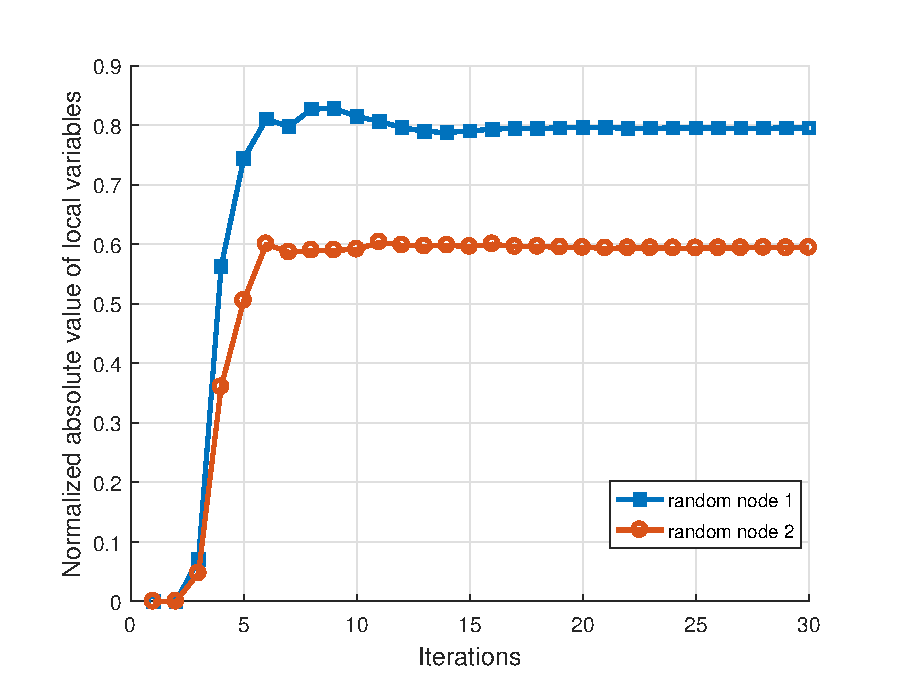
\includegraphics[width=12cm]{graphics/4-heuristic-dist/distributed_local_vars_convergence}}
	\caption{نحوه‌ همگرا شدن متغیر محلی در دو گره تصادفی در روش توزیع‌شده}
	\label{fig:distributed_local_vars_convergence}
\end{figure}

	ابتدا نحوه‌ی همگرایی در روش توزیع شده را بررسی می‌کنیم. در \cref{fig:distributed_local_vars_convergence} نحوه همگرایی برای دو گره تصادفی از شبکه در روش توزیع شده به نمایش گذاشته شده‌است. در این نمودار اندازه متغیر محلی برای این دوگره در طول زمان نشان داده شده‌است. 
	
\begin{figure}[h!]
	\centerline{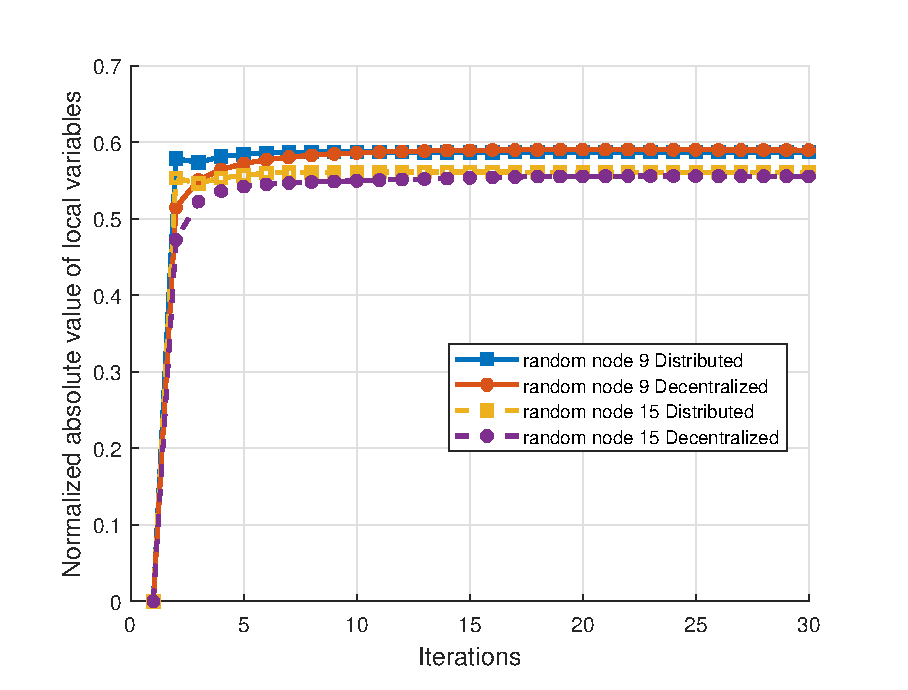
\includegraphics[width=12cm]{graphics/4-heuristic-dist/distributed_decent_local_vars_convergence}}
	\caption{نحوه‌ همگرا شدن اندازه‌ی متغیر  محلی مسئله در دو روش توزیع‌شده و غیرمتمرکز برای دوگره تصادفی}
	\label{fig:distributed_decent_local_vars_convergence}
\end{figure}

	در \cref{fig:distributed_decent_local_vars_convergence}	نحوه‌ همگرایی متغیر محلی در دو روش غیرمتمرکز و توزیع‌شده مقایسه شده‌است. همانطور که دیده می‌شود در روش غیرمتمرکز سرعت همگرایی اندکی بیشتر است، که دلیل آن وجود واحد هدایت‌گر\LTRfootnote{Coordinator} در روش غیرمتمرکز است که باعث می‌شود سرعت همگرایی بیشتر شود و همچنین نحوه همگرایی صاف‌تر باشد. 

\begin{figure}[h!]
	\centerline{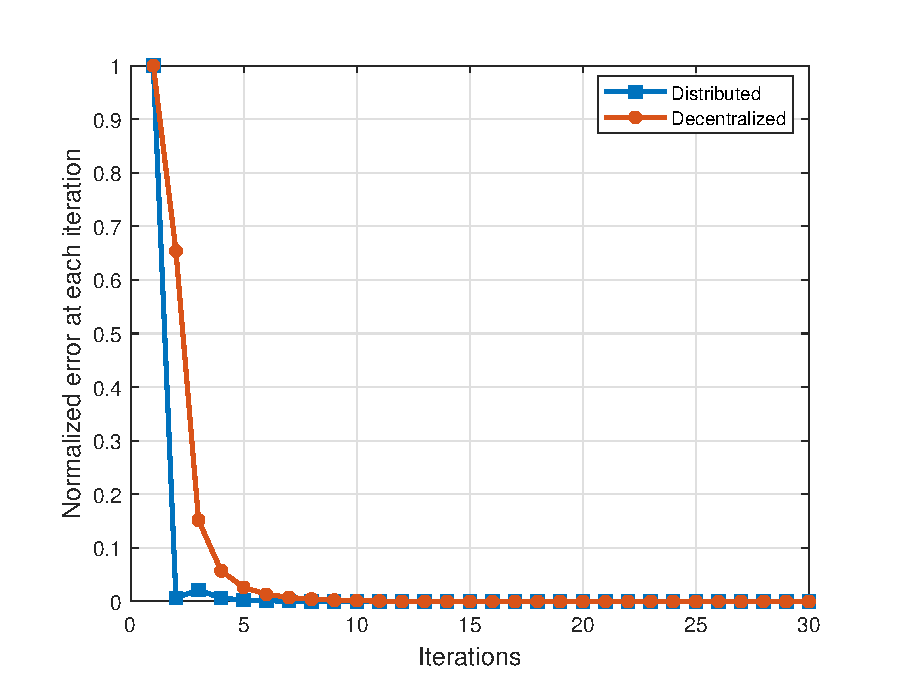
\includegraphics[width=12cm]{graphics/4-heuristic-dist/error_convergence_dist_decent}}
	\caption{نحوه همگرا شدن مقدار خطا در دو روش توزیع‌شده و غیرمتمرکز}
	\label{fig:error_convergence_dist_decent}
\end{figure}

	در \cref{fig:error_convergence_dist_decent} نیز نحوه همگرایی میزان خطا در دو روش غیرمتمرکز و توزیع‌شده به نمایش گذاشته شده‌است. در این نمودار در هر مرحله اختلاف مقدار تابع هدف با مرحله قبل به صورت خطا در نظر گرفته شده‌است که این خطا به صورت یکه شده نمایش داده شده‌است. 

\begin{figure}[h!]
	\centerline{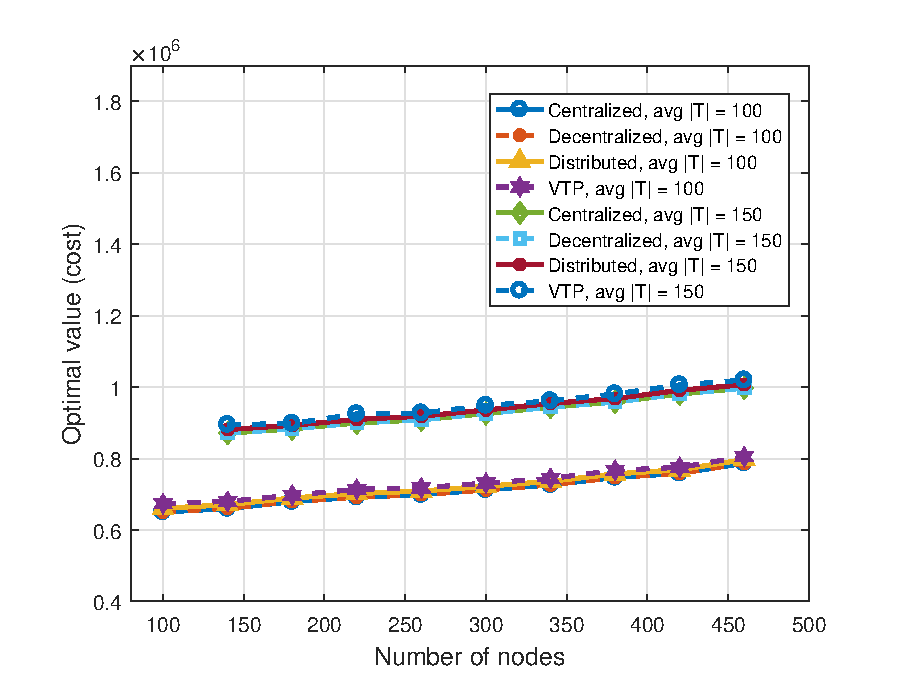
\includegraphics[width=12cm]{graphics/4-heuristic-dist/optimization_value_per_number_of_nodes_all_solutions}}
	\caption{مقدار تابع هدف (هزینه) برای چهار روش مختلف دربرابر تعداد کل گره‌های شبکه}
	\label{fig:optimization_value_per_number_of_nodes_all_solutions}
\end{figure}

	در شبیه‌سازی بعدی که در \cref{fig:optimization_value_per_number_of_nodes_all_solutions} دیده می‌شود هر چهار روش موجود بر روی شبکه اجرا شده‌است، همانطور که از این نمودار دیده می‌شود مقدار تابع هدف در دو راه‌حل متمرکز و غیرمتمرکز بهینه است و در راه حل توزیع‌شده نیز با فاکتور دلخواه $\epsilon$ قابل کنترل است، اما در مورد راه‌حل اکتشافی می‌بینیم که این راه‌حل جواب زیربهینه را می‌دهد. 
\begin{figure}[h!]
	\centerline{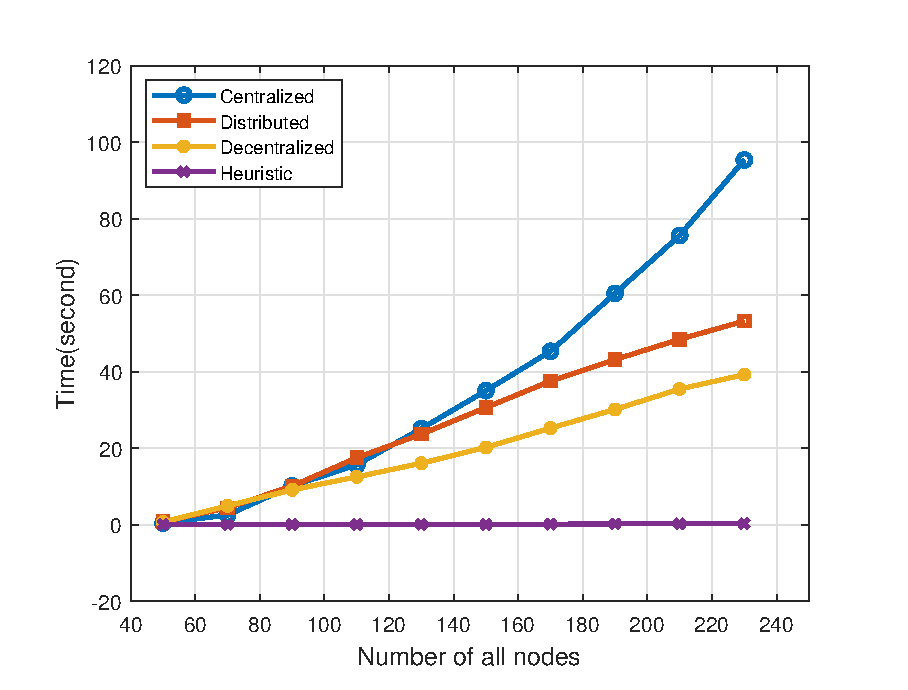
\includegraphics[width=12cm]{graphics/4-heuristic-dist/time_of_convergence}}
	\caption{زمان نسبی آماده شدن جواب نهایی در چهار روش مختلف دربرابر تعداد  گره‌های شبکه}
	\label{fig:time_of_convergence}
\end{figure}

	آخرین تحلیل مربوط به زمان آماده شدن جواب در چهار راه‌حل ارائه‌شده در این پایان‌نامه است. سعی شده است که شبیه‌سازی‌ها در شرایط کاملا یکسان انجام شود، ازجمله میزان حافظه موجود بر روی دستگاه کامپیوتری که تست ها برروی انجام شده‌است و یا دمای پردازنده در هنگام تست و ... . همانطور که دیده می‌شود به وضوح زمان انجام محاسبات در راه‌حل اکتشافی کم است. در مورد دو راه حل غیرمتمرکز و توزیع‌شده نیز ذکر این نکته لازم است که شرایط واقعی شبیه‌سازی زمانی‌است که محاسبات در گره‌های مختلف و به‌صورت همزمان انجام شود در حالیکه در تست‌های انجام شده به دلیل محدودیت منابع کلیه شبیه‌سازی‌ها بر روی یک دستگاه انجام شده‌است که این خود باعث می‌شود خاصیت اصلی این دو روش به خوبی دیده نشود، با این وجود در \cref{fig:time_of_convergence} دیده می‌شود که زمان نسبی آماده شدن جواب در سه روش غیرمتمرکز، توزیع‌شده و اکتشافی به صورت خطی نسبت به اندازه توپولوژی مسئله است.
	
	\section{جمع‌بندی و نتیجه‌گیری}
	در این فصل دو روش دیگر برای حل مسئله اصلی ارائه‌شد. 
	روش اول یک روش کاملا توزیع شده‌است که مسئله بین تمام گره‌های پردازشی تقسیم می‌شود و از قدرت پردازشی آن‌ها برای حل مسئله کمک گرفته می‌شود.
	روش دوم یک راه‌حل اکتشافی مبتی بر الگوریتم ویتربی بود که مسئله اصلی را بدون نیاز به خطی‌سازی و به صورت اکتشافی حل می‌کند. 
	هردو روش ارائه شده در این فصل جواب زیر‌بهینه ارائه می‌کردند. 
	در قسمت نتایج دیده شد که هر دوروش در زمان خطی به نتیجه می‌رسند و چهار روش ارائه شده در این پایان‌نامه از جنبه‌های مختلف با یکدیگر مقایسه شد. 


%\chapter{نتیجه‌گیری و کار‌های آینده}\label{chap:conclusion}
  \thispagestyle{empty}
  در این فصل ابتدا مروری داریم بر کار‌های انجام شده در این پایان نامه و سپس برخی از جهت‌های تحقیقاتی ممکن برای ادامه‌ی این فعالیت پژوهشی بیان خواهند شد.

  \section{خلاصه و جمع‌بندی}
    در این پایان‌نامه، ابتدا به معرفی اینترنت اشیاء و کاربرد‌های آن در شهر هوشمند پرداختیم.
    پس از آن برخی خدمات شهر هوشمند را برشمردیم.
    سپس به معرفی پردازش لبه و مه و دلایل برتری آن‌ها نسبت به پردازش ابری پرداختیم.
    در ادامه کار‌های انجام شده در اختصاص منابع در شبکه اینترنت اشیاء را بررسی کردیم.

    در \cref{chap:3-system_model_centralized_decentralized} صورت مسئله تخصیص منابع جهت پردازش وظیفه‌ها به صورت یک مسئله بهینه‌سازی مدل‌سازی شد. 
    در این نوع از تخصیص منابع، منابع پردازشی به تعدادی وظیفه اختصاص پیدا می‌کنند.
    در این فصل مسئله تخصیص منابع به صورت یک مسئله بهینه سازی فرمول بندی شد که هدف آن کمینه کردن مجموع هزینه پردازشی در کل گره‌های شبکه است.
    با توجه به حل دشوار مسئله مورد نظر در ابتدا این مسئله خطی‌سازی شد. جواب بهینه مسئله به روش متمرکز به دست آمد.
    در ادامه یک روش غیرمتمرکز برای حل مسئله ارائه شد و در نهایت میزان پیچیدگی و نحوه همگرایی در این روش بررسی شد. در آخر نتایج مقایسه‌ای برای این دو روش ارائه شد.

    در \cref{chap:4-heuristic_distributed} ابتدا صورت مسئله غیرخطی اولیه بازنویسی شد.
    به کمک الگوریتم ویتربی یک راه‌حل اکتشافی برای حل مسئله اولیه به صورت زیر‌بهینه ارائه شد.
	در ادامه یک روش توزیع‌شده نیز برای حل مسئله خطی‌‌شده ارائه شد. این روش نیز جواب زیربهینه ارائه می‌کرد. 
    پس از بررسی همگرایی و پیچیدگی دو الگوریتم ارائه شده، شبیه‌سازی‌هایی برای بررسی آن‌ها ارائه شد.
    درنهایت چهار روش موجود در این پایان نامه از نظر زمان رسیدن به جواب مقایسه شد که مشخص شد روش اکتشافی سریع‌ترین روش است. 

  \section{کار‌های آینده}
    در این قسمت چند پیشنهاد برای ادامه این کار مطرح می‌کنیم.
  
  اولین پیشنهاد که به صورت یک پیشنهاد عملی است این است که دو روش غیرمتمرکز و توزیع‌شده به عنوان قراردادهای هوشمندی در شبکه زنجیره‌‌بلوک\LTRfootnote{Blockchain} عملیاتی شوند. برای این‌کار لازم است که کلیه گره‌های موجود در شبکه به عنوان یک گره در شبکه زنجیره‌بلوک در نظر گرفته‌شوند. برای ایجاد امنیت بیشتر در این شبکه می‌توان از زنجیره‌های بلوک خصوصی استفاده کرد.
  
    به عنوان پیشنهاد دوم، با ترکیب کردن این مدل‌ها با شبکه‌های مبتنی بر نرم‌افزار\LTRfootnote{Software Defined Networks (SDN)} می‌توان به مدل بهتری رسید.
    همچنین ترکیب این کار با تخصیص منابع رادیوی برای انتقال داده‌های حسگر‌ها و فعال کننده‌ها هم می‌تواند به واقعی‌تر شدن مدل ارائه شده کمک کند.

    به عنوان پیشنهاد آخر، در مدل ارائه شده در \cref{chap:3-system_model_centralized_decentralized} می‌توان مسئله را به صورت یک بازی\LTRfootnote{Game} تعریف کرد و از روش‌های حل مسئله برای این دسته از مسائل استفاده کرد. 

% مراجع
\pagestyle{empty}
{
\onehalfspacing
\bibliographystyle{ieeetr-fa}%{acm-fa}%{chicago-fa}%{plainnat-fa}%
\bibliography{references}
}
\printindex
% !TeX root=main.tex
% در این فایل، عنوان پایان‌نامه، مشخصات خود و چکیده پایان‌نامه را به انگلیسی، وارد کنید.

%%%%%%%%%%%%%%%%%%%%%%%%%%%%%%%%%%%%

\begin{latin}
  %\latinfaculty{}
  \latindepartment{School of Electrical and Computer Engineering}
  \latinsubject{Electrical Engineering}
  \latinfield{Communication Engineering}
  \latintitle{Distributed Intelligence in IoT Networks}
  \firstlatinsupervisor{Dr. Vahid Shah-Mansouri}
  %\secondlatinsupervisor{Second Supervisor}
  %\firstlatinadvisor{First Advisor}
  %\secondlatinadvisor{Second Advisor}
  \latinname{Mohammad}
  \latinsurname{Mahmoodian}
  \latinthesisdate{September 2020}
  
  \latinkeywords{Internet of Things (IoT), Smart City, edge computing, fot computing, cloud computing, distributed optimization, resource allocation}
  
  \en-abstract{
%	The smart city is one of the most important applications of the Internet of Things (IoT) that has recently been considered by researchers. In the smart city, the goal is for all available devices to be able to connect to the Internet, so that all information exchange takes place within the network.
%	The information generated by these devices first needs to be processed and analyzed. Therefore, this information must be sent to the processing resources and the result of the processing must be returned to the relevant devices in the form of decisions.
  }

  \cleartoleftpage
  \latinabstractPage
  \cleartoleftpage
  \latinfirstPage
\end{latin}

\label{LastPage}

\end{document}
